%%%%%%%%%%%%%%%%%%%%%%%%%%%%%%%%%%%%%%%%%
% Masters/Doctoral Thesis 
% LaTeX Template
% Version 2.5 (27/8/17)
%
% This template was downloaded from:
% http://www.LaTeXTemplates.com
%
% Version 2.x major modifications by:
% Vel (vel@latextemplates.com)
%
% This template is based on a template by:
% Steve Gunn (http://users.ecs.soton.ac.uk/srg/softwaretools/document/templates/)
% Sunil Patel (http://www.sunilpatel.co.uk/thesis-template/)
%
% Template license:
% CC BY-NC-SA 3.0 (http://creativecommons.org/licenses/by-nc-sa/3.0/)
%
%%%%%%%%%%%%%%%%%%%%%%%%%%%%%%%%%%%%%%%%%

%----------------------------------------------------------------------------------------
%	PACKAGES AND OTHER DOCUMENT CONFIGURATIONS
%----------------------------------------------------------------------------------------

\documentclass[
11pt, % The default document font size, options: 10pt, 11pt, 12pt
%oneside, % Two side (alternating margins) for binding by default, uncomment to switch to one side
english, % ngerman for German
doublespacing, % line spacing, alternatives: singlespacing, onehalfspacing or doublespacing
%draft, % Uncomment to enable draft mode (no pictures, no links, overfull hboxes indicated)
%nolistspacing, % If the document is onehalfspacing or doublespacing, uncomment this to set spacing in lists to single
%liststotoc, % Uncomment to add the list of figures/tables/etc to the table of contents
%toctotoc, % Uncomment to add the main table of contents to the table of contents
%parskip, % Uncomment to add space between paragraphs
%nohyperref, % Uncomment to not load the hyperref package
headsepline, % Uncomment to get a line under the header
%chapterinoneline, % Uncomment to place the chapter title next to the number on one line
%consistentlayout, % Uncomment to change the layout of the declaration, abstract and acknowledgements pages to match the default layout
]{MastersDoctoralThesis} % The class file specifying the document structure

\usepackage[utf8]{inputenc} % Required for inputting international characters
\usepackage[T1]{fontenc} % Output font encoding for international characters

\usepackage{mathpazo} % Use the Palatino font by default

\usepackage[backend=bibtex,style=authoryear,natbib=true]{biblatex} % Use the bibtex backend with the authoryear citation style (which resembles APA)
\addbibresource{example,bib_game,bib_tech,bib_mcts,bib_moba,bib_mywork,bib_rl,bib_eomm,bib_dda,bib_churn,bib_recom} % The filename of the bibliography
% \bibliographystyle{apalike}


\usepackage[autostyle=true]{csquotes} % Required to generate language-dependent quotes in the bibliography

\usepackage{xcolor}
%\pagecolor{lightgray!40}
\usepackage{ifdraft}
% \ifoptionfinal{}{\pagecolor[HTML]{FDF6E3}}
% \ifoptionfinal{}{\pagecolor[HTML]{F8DF9C}}
\ifoptionfinal{}{\pagecolor[HTML]{cac4b5}}

% math
\usepackage{amsmath,amssymb,amsfonts}

% For highlighting
\usepackage{color,soul}

% table row spacing
\newcommand{\ra}[1]{\renewcommand{\arraystretch}{#1}}

% For bold vectors
\newcommand{\vect}[1]{\boldsymbol{#1}}

% For argmax
\DeclareMathOperator*{\argmax}{arg\,max}
\DeclareMathOperator*{\argmin}{arg\,min}

% merge cell vertically in table
\usepackage{multirow}

% itermize no left margin
\usepackage{enumitem}

% For algorithms
\usepackage[ruled]{algorithm2e} 

% URL line break but doesn't work all the time
\usepackage{etoolbox}
\appto\UrlBreaks{\do\-}

% adjustwidth in table for over wide tables
% see https://stackoverflow.com/questions/722613/centering-a-table-wider-than-the-text-column
\usepackage{chngpage}

%%%%%%%%%%%%%%%%%%%%%%%%%%%%%%%%%%%%%%%%%%%%%%%%%%%%%%%%%%%%%%%%%%%
%                 hyperlink for whole citation                    %
%%%%%%%%%%%%%%%%%%%%%%%%%%%%%%%%%%%%%%%%%%%%%%%%%%%%%%%%%%%%%%%%%%%
\DeclareCiteCommand{\cite}
  {\usebibmacro{prenote}}
  {\usebibmacro{citeindex}%
   \printtext[bibhyperref]{\usebibmacro{cite}}}
  {\multicitedelim}
  {\usebibmacro{postnote}}

\DeclareCiteCommand*{\cite}
  {\usebibmacro{prenote}}
  {\usebibmacro{citeindex}%
   \printtext[bibhyperref]{\usebibmacro{citeyear}}}
  {\multicitedelim}
  {\usebibmacro{postnote}}

\DeclareCiteCommand{\parencite}[\mkbibparens]
  {\usebibmacro{prenote}}
  {\usebibmacro{citeindex}%
    \printtext[bibhyperref]{\usebibmacro{cite}}}
  {\multicitedelim}
  {\usebibmacro{postnote}}

\DeclareCiteCommand*{\parencite}[\mkbibparens]
  {\usebibmacro{prenote}}
  {\usebibmacro{citeindex}%
    \printtext[bibhyperref]{\usebibmacro{citeyear}}}
  {\multicitedelim}
  {\usebibmacro{postnote}}

\DeclareCiteCommand{\footcite}[\mkbibfootnote]
  {\usebibmacro{prenote}}
  {\usebibmacro{citeindex}%
  \printtext[bibhyperref]{ \usebibmacro{cite}}}
  {\multicitedelim}
  {\usebibmacro{postnote}}

\DeclareCiteCommand{\footcitetext}[\mkbibfootnotetext]
  {\usebibmacro{prenote}}
  {\usebibmacro{citeindex}%
   \printtext[bibhyperref]{\usebibmacro{cite}}}
  {\multicitedelim}
  {\usebibmacro{postnote}}

\DeclareCiteCommand{\textcite}
  {\boolfalse{cbx:parens}}
  {\usebibmacro{citeindex}%
   \printtext[bibhyperref]{\usebibmacro{textcite}}}
  {\ifbool{cbx:parens}
     {\bibcloseparen\global\boolfalse{cbx:parens}}
     {}%
   \multicitedelim}
  {\usebibmacro{textcite:postnote}}
%---------------------------------------------------------------------------


%----------------------------------------------------------------------------------------
%	MARGIN SETTINGS
%----------------------------------------------------------------------------------------

\geometry{
	paper=a4paper, % Change to letterpaper for US letter
	inner=2.5cm, % Inner margin
	outer=3.8cm, % Outer margin
	bindingoffset=.5cm, % Binding offset
	top=1.5cm, % Top margin
	bottom=1.5cm, % Bottom margin
	%showframe, % Uncomment to show how the type block is set on the page
}

%---------------------------------------------------------------------------------------
%	THESIS INFORMATION
%----------------------------------------------------------------------------------------

% I don't want to say my thesis is just adaptation techniques. Adaptation techniques

% original: Pre-Match Recommendations for Influencing Match Outcomes and Player Engagement in Video Games
\thesistitle{Recommendation Systems for Influencing Player Competence and Engagement in Pre-Match of Match-Based Games} % Your thesis title, this is used in the title and abstract, print it elsewhere with \ttitle
\supervisor{Magy Seif El-Nasr (Advisor)} % Your supervisor's name, this is used in the title page, print it elsewhere with \supname
\supervisorone{Christopher Amato}
\supervisortwo{Seth Cooper}
\supervisorthree{Yizhou Sun}
\examiner{} % Your examiner's name, this is not currently used anywhere in the template, print it elsewhere with \examname
\degree{Doctor of Philosophy} % Your degree name, this is used in the title page and abstract, print it elsewhere with \degreename
\author{Zhengxing Chen} % Your name, this is used in the title page and abstract, print it elsewhere with \authorname
\addresses{} % Your address, this is not currently used anywhere in the template, print it elsewhere with \addressname

\subject{Computer Sciences} % Your subject area, this is not currently used anywhere in the template, print it elsewhere with \subjectname
\keywords{} % Keywords for your thesis, this is not currently used anywhere in the template, print it elsewhere with \keywordnames
\university{Northeastern University} % Your university's name and URL, this is used in the title page and abstract, print it elsewhere with \univname
\department{College of Information and Computer Science} % Your department's name and URL, this is used in the title page and abstract, print it elsewhere with \deptname
\group{Research Group Name} % Your research group's name and URL, this is used in the title page, print it elsewhere with \groupname
\faculty{faculty name} % Your faculty's name and URL, this is used in the title page and abstract, print it elsewhere with \facname

\AtBeginDocument{
\hypersetup{pdftitle=\ttitle} % Set the PDF's title to your title
\hypersetup{pdfauthor=\authorname} % Set the PDF's author to your name
\hypersetup{pdfkeywords=\keywordnames} % Set the PDF's keywords to your keywords
}

\begin{document}

\frontmatter % Use roman page numbering style (i, ii, iii, iv...) for the pre-content pages

\pagestyle{plain} % Default to the plain heading style until the thesis style is called for the body content

%----------------------------------------------------------------------------------------
%	TITLE PAGE
%----------------------------------------------------------------------------------------

\begin{titlepage}
\begin{center}

%\vspace*{.06\textheight}
{\scshape\LARGE \univname\par}\vspace{0.5cm} % University name
\textsc{\Large Doctoral Dissertation}\\[0.5cm] % Thesis type

\HRule \\[0.4cm] % Horizontal line
{\huge \bfseries \ttitle\par}\vspace{0.4cm} % Thesis title
\HRule \\[1.5cm] % Horizontal line
 
\begin{minipage}[t]{0.4\textwidth}
\begin{flushleft} \large
\emph{Author:}\\
{\authorname} % Author name - remove the \href bracket to remove the link
\end{flushleft}
\end{minipage}
\begin{minipage}[t]{0.4\textwidth}
\begin{flushright} \large
\emph{Committee:} \\
{\supname} \\ % Supervisor name - remove the \href bracket to remove the link  
{\supnameone} \\
{\supnametwo} \\ 
{\supnamethree} 
\end{flushright}
\end{minipage}\\[3cm]
 
\vfill

\large \textit{A dissertation submitted in fulfillment of the requirements\\ for the degree of \degreename}\\[0.3cm] % University requirement text
\textit{in the}\\[0.4cm]
\deptname\\\univname\\[2cm] % department name and university name
 
\vfill

{\large \today}\\[4cm] % Date
%\includegraphics{Logo} % University/department logo - uncomment to place it
 
\vfill
\end{center}
\end{titlepage}

%----------------------------------------------------------------------------------------
%	DECLARATION PAGE
%----------------------------------------------------------------------------------------

\begin{declaration}
\addchaptertocentry{\authorshipname} % Add the declaration to the table of contents
\noindent I, \authorname, declare that this dissertation titled, \enquote{\ttitle} and the work presented in it are my own. I confirm that:

\begin{itemize} 
\item This work was done wholly or mainly while in candidature for a research degree at this University.
\item Where any part of this dissertation has previously been submitted for a degree or any other qualification at this University or any other institution, this has been clearly stated.
\item Where I have consulted the published work of others, this is always clearly attributed.
\item Where I have quoted from the work of others, the source is always given. With the exception of such quotations, this dissertation is entirely my own work.
\item I have acknowledged all main sources of help.
\item Where the dissertation is based on work done by myself jointly with others, I have made clear exactly what was done by others and what I have contributed myself.\\
\end{itemize}
 
\noindent Signed:\\
\rule[0.5em]{25em}{0.5pt} % This prints a line for the signature
 
\noindent Date:\\
\rule[0.5em]{25em}{0.5pt} % This prints a line to write the date
\end{declaration}

\cleardoublepage

%----------------------------------------------------------------------------------------
%	QUOTATION PAGE
%----------------------------------------------------------------------------------------

% \vspace*{0.2\textheight}

% \noindent\enquote{\itshape Thanks to my solid academic training, today I can write hundreds of words on virtually any topic without possessing a shred of information, which is how I got a good job in journalism.}\bigbreak

% \hfill Dave Barry

%----------------------------------------------------------------------------------------
%	ABSTRACT PAGE
%----------------------------------------------------------------------------------------

\begin{abstract}
\addchaptertocentry{\abstractname} % Add the abstract to the table of contents

For years, video games have garnered the attention of people worldwide, providing a unique environment for entertainment, story adventure, scientific learning, etc. With the increase in popularity of video games, a critical question arises: how to keep player engaged.  

In this dissertation, I address player engagement through developing recommendation systems that give players the ability to make informed choices concerning in-game elements, such as which characters to play as, which items to equip with, or which opponents to play against. The underlying assumption here is that controlling what in-game elements to present to players could influence their choices of in-game elements, the way they play, competence they perceive, and eventually their engagement. I particularly focus on online match-based games, where players competitively play against others, and further, I specifically target pre-match stage choices. 

Within this domain, I propose to study two related research questions. The first research question is concerned with development of effective and efficient recommendation systems for suggesting winning-effective in-game elements, in both one-vs-one and team-vs-team settings. We assume these systems could help players who fail to select winning-effective items regain competence and consequently improve their engagement, since numerous theoretical foundations, such as Self Determination Theory and Flow, have supported that player competence is an important part of engagement. 

To this end, I first propose \textit{Q-DeckRec} for recommending winning-effective decks, a set of cards seen as the starting items, in one-vs-one Collectible Card Games (CCGs). Q-DeckRec deals with the challenge of using minimal computational resources to identify a winning-effective deck against an opponent stereotype from a large number of deck candidates. Previous works using heuristic searches require intense manual works and those using metaheuristic searches require expensive computational resources to enable large-scale or real-time usage. Based on simulations operated by AI bots, Q-DeckRec, after a training phase, is able to recommend equally or more winning-effective decks with much less computational resource in terms of CPU time compared to other methods. 

I also propose \textit{DraftArtist} for recommending winning-effective characters in Multi-player Online Battle Arena (MOBA) games, which are played team-vs-team. The challenge beyond the one-vs-one setting is that other players' character selection strategies bring a large number of possibilities and uncertainty and need to be taken into accounts; a desirable character recommendation system should predict what other players will select and efficiently search for characters which synergize the teammates' and counter the opponents'. Existing methods are not effective enough to approach the character optimal for victory for the player's whole team. Using a match outcome prediction model trained on real data, we find that teams following our recommendation algorithm for character selection have higher predicted win rates against teams constructed by other character selection strategies, while our algorithm still maintains sufficient efficiency to be deployed in real-world scenarios.

The second research question I study is to design in-game element recommendation systems which directly improve player engagement using data-driven approaches. I propose to study opponent recommendation, also known as matchmaking, a special case in which the goal is to connect multiple players to form online matches and players themselves are the subject of recommendations. I propose \textit{Engagement-Optimized Matchmaking} (EOMM) in which projected match outcomes between paired players would optimize all involved players' engagement measured by churn risks (i.e., quiting probabilities). To our best knowledge, our proposed matchmaking method is the first that have formally treated matchmaking as an optimization problem to maximize player engagement quantitatively. We build a player behavior simulation system based on real data, showing significant improvement in enhancing population-wise player engagement by EOMM against other matchmaking methods.

The overall contribution of my dissertation is the enrichment of arsenal of recommendation techniques in (1) winning-effective
in-game element recommendation and (2) in-game element recommendation directly used for improving player engagement in data-driven approaches. Since video games possess a variety of forms of in-game elements, the future direction will be to study systems tailored for more specific types of in-game elements, as well as those which can make central decisions on different types of recommendations for any particular player.


% Such variety and richness     match outcomes are believed to be closely related to player engagement and revenues made by game companies. Based on individual players' information and game contexts, personalized recommendation is one family of proposed methods, wherein dynamic game contents are recommended to players in order to influence their win rates. 

% investigating the close relationship in-game competence and player engagement. 

% As there can be various goals for influencing game outcomes and video games sport different designs and in-game elements, I am not able to examine every place where in-game element recommendation can be applied. Rather, I focus on the following boundaries delimiting my research.

% thus Q-DeckRec is designed to be suitable for large-scale or real-time recommendation application.

% i.e., the level of player competence manipulation is directly linked to player engagement. 

% in which an optimization objective is designed to arbitrate the strength of competence manipulation for every player and benefit the overall engagement as the end goal. Specifically, 

%  and in most cases they passively accept what they are matched with

% \linebreak 

% Particularly, I study how to design recommendation systems for the optimization of population-wise player engagement.
% * <czxttkl@gmail.com> 2018-07-25T10:02:11.856Z:
%
% ^.
% * <czxttkl@gmail.com> 2018-07-25T10:02:09.838Z:
%
% ^.

% EOMM presents a new way of thinking opponent recommendation as an optimization problem which can be solved through a graph matching algorithm. 

% The connections between the three proposed recommendation systems are as follows. All the systems use recommendations as a means to influence game outcomes. They can be indirectly or directly used to improve player engagement. The starting item and character recommendation systems aim for increasing the win rate for one player, which can be seen as an indirect step to improve player engagement because they need to work with other systems which decide when to deliver recommendations, while EOMM directly operates on the optimization of population-wise player engagement as the criterion for influencing game outcomes for multiple players.

% In each match, human players (and possibly computer agents) compete with each other.
% First, I focus on recommendations in the pre-match stage in video games played based on small sessions called matches. In the pre-match stage, some in-game elements determined before the match starts could already have an impact on the final match outcome and player engagement.
% Second, I focus on two goals for employing recommendations to influence game outcomes: to increase a player's win rate and to increase player engagement. The two goals are progressive, in a sense that increasing a player's win rate is an intermediate and indirect step to improve player engagement.
% Third, I focus on the recommendations of three specific types of in-game elements: starting items, in-game characters and opponents. These are very common in-game elements in video games nowadays. However, identifying right recommendations of them face different challenges: (1) I propose  personalized recommendation system for suggesting starting items  to optimal for a player's win rate. It could be a challenging task for the player to choose winning-effective starting items since a large amount of choices could be available depending on the strategies of the player and the opponent; (2) I propose an in-game character recommendation system for suggesting team-based video games with the goal to maximize a player's win rate.Last, I propose a matchmaking system for opponent recommendation, in which expected match outcomes within recommended opponents optimize all involved players' engagement. 

% A distinctive feature of personalized recommendation in PvP games is that influencing one's winning probability will adversely change that of the opponent(s) who are human players too. The initial item recommendation system exemplifies \textit{how} match outcomes can be affected positively \textit{from one side}, while the opponent recommendation system exemplifies not only \textit{how} but also \textit{how much} match outcomes should be influenced when we consider \textit{a population of players}.



\end{abstract}

%----------------------------------------------------------------------------------------
%	ACKNOWLEDGEMENTS
%----------------------------------------------------------------------------------------

\begin{acknowledgements}
\addchaptertocentry{\acknowledgementname} % Add the acknowledgements to the table of contents
I would like to thank my advisor Prof. Magy Seif El-Nasr for her patience, motivation, and knowledge. I could not forget our first meeting where she shed lights on game analytics and encouraged me to take on this direction. Without her support over the last five years, I could never have been so fortunate to carve a niche in the interdisciplinary research area of video games and artificial intelligence.

My sincere thanks also go to my dissertation committee members: Prof. Christopher Amato, Prof. Yizhou Sun, and Prof. Seth Cooper. They provided me with enormous helps and inspired my research in diverse perspectives. 

I am grateful to all collaborators I worked with during my research as well as colleagues I met during my internships at Electronic Arts, eBay, Google, and Facebook. My special gratefulness goes to Prof. Truong-Huy Nguyen for suggesting me PhD and life advice, and Dr. Su Xue and Dr. John Kolen for fostering my incredible internship experience at Electronic Arts.

I thank Prof. Karl Lieberherr and Prof. Stephen Intille for their kind helps in the first year of my PhD. I also thank all my friends and lab mates for their support, understanding, and encouragement.

I cannot thank more than enough to my parents and grandparents, who have taught me to become kind, strong, and wise throughout my whole life.

Last but by no means least, I would like to express my thankfulness to my wife, Shiyun, for accompanying me through the so far most challenging yet most memorable time in my life. We will have much more adventure to experience in the future.
\end{acknowledgements}

%----------------------------------------------------------------------------------------
%	LIST OF CONTENTS/FIGURES/TABLES PAGES
%----------------------------------------------------------------------------------------

\tableofcontents % Prints the main table of contents

\listoffigures % Prints the list of figures

\listoftables % Prints the list of tables

% %----------------------------------------------------------------------------------------
% %	ABBREVIATIONS
% %----------------------------------------------------------------------------------------

% \begin{abbreviations}{ll} % Include a list of abbreviations (a table of two columns)

% \textbf{LAH} & \textbf{L}ist \textbf{A}bbreviations \textbf{H}ere\\
% \textbf{WSF} & \textbf{W}hat (it) \textbf{S}tands \textbf{F}or\\

% \end{abbreviations}

% %----------------------------------------------------------------------------------------
% %	PHYSICAL CONSTANTS/OTHER DEFINITIONS
% %----------------------------------------------------------------------------------------

% \begin{constants}{lr@{${}={}$}l} % The list of physical constants is a three column table

% % The \SI{}{} command is provided by the siunitx package, see its documentation for instructions on how to use it

% Speed of Light & $c_{0}$ & \SI{2.99792458e8}{\meter\per\second} (exact)\\
% %Constant Name & $Symbol$ & $Constant Value$ with units\\

% \end{constants}

% %----------------------------------------------------------------------------------------
% %	SYMBOLS
% %----------------------------------------------------------------------------------------

% \begin{symbols}{lll} % Include a list of Symbols (a three column table)

% $a$ & distance & \si{\meter} \\
% $P$ & power & \si{\watt} (\si{\joule\per\second}) \\
% %Symbol & Name & Unit \\

% \addlinespace % Gap to separate the Roman symbols from the Greek

% $\omega$ & angular frequency & \si{\radian} \\

% \end{symbols}

% %----------------------------------------------------------------------------------------
% %	DEDICATION
% %----------------------------------------------------------------------------------------

% \dedicatory{For/Dedicated to/To my\ldots} 

%----------------------------------------------------------------------------------------
%	THESIS CONTENT - CHAPTERS
%----------------------------------------------------------------------------------------

\mainmatter % Begin numeric (1,2,3...) page numbering

\pagestyle{thesis} % Return the page headers back to the "thesis" style

% Include the chapters of the thesis as separate files from the Chapters folder
% Uncomment the lines as you write the chapters

% Chapter Template

\chapter{Introduction} % Main chapter title

\label{chapter:intro} % Change X to a consecutive number; for referencing this chapter elsewhere, use \ref{ChapterX}

\section{Motivation and Research Question}\label{chap1:motiv}

The world has witnessed a gallery of video games that manage to make people addicted into playing day and night. The series of \textit{Super Mario Bros.} (Nintendo Co. Ltd) have sold over 160 million since the 1980s \cite{mariosale}. Players enjoy the excitement and fulfillment of passing through game levels designed with various challenges. \textit{League of Legends}, a 5-vs-5 online competitive game, has 90 million users registered, 27 million unique daily players and 7.5 million concurrent users at peak \cite{lol_fanbase,lol_27million}. The game is characteristized by competition, collaboration and strategies that players are hard to experience in the real world. Recently, \textit{Pok\'{e}mon Go} (Niantic, Inc.) has swept the globe with more than 500 million downloads \cite{pokemongo}, triggering the crowd to walk on the street to interact with the game. At the same time, the viewership of video games has also grown rapidly. e-Sports, a subset of highly competitive video games, was estimated to have hundreds of million viewership in 2017 and projected to still grow at 12\% each year~\cite{superdata2017}. Besides being commonly perceived as a means of entertainment, video games have also been utilized for various purposes, such as promoting aesthetic appreciation~\cite{jarvinen2008understanding}, health awareness~\cite{shiyko2016effects}, science learning~\cite{cooper2013increasing}, and socialization~\cite{ferguson2013friends}.

As video games continue to penetrate an increasing number of fields for improving the wellness of our society, one question arises naturally: \textit{how can we keep players engaged?} Indeed, without player engagement, video games could not serve their purposes ranging from entertainment to promoting science learning. Poor player engagement would not only hurt the gaming experience of players, but also revenues by game companies, as nowadays video games have become a highly valuable market worth hundreds of billions of dollars~\cite{today_video_game_market}.

Therefore, player engagement becomes a critical topic for research, with its importance reflected by a large body of literatures (e.g.,~\cite{boyle2012engagement,schoenau2011player,choi2004people,brockmyer2009development}). We adopt the most straightforward definition of player engagement as the "continuation desire" to play a game repeatedly during play or over a longer period of time~\cite{schoenau2011player}, while the desire may be explained by numerous different theories; famous examples include Self-Determination theory~\cite{przybylski2010motivational,ryan2006motivational} which associates players' motives to continue playing with their needs for competence, autonomy and relatedness, and Flow theory~\cite{sweetser2005gameflow,flow1990psychology,chen2007flow} which argues that one important ingredient of player engagement is the optimal match between challenges in the game and their skills.

While player engagement could derive from many factors as suggested by the rich literature, one factor can be deduced from numerous theories that has a close relationship with player engagement: \textbf{game outcomes}. In my thesis, I refer a game outcome generally to any possible outcome in a game indicating the player's progress, such as wins, losses, level-ups, and milestones achieved. According to Flow theory~\cite{sweetser2005gameflow,flow1990psychology,chen2007flow}, part of player engagement comes from challenges which match the player's skill level and keep at an appropriate pace. Similarly, competence in Self-Determination theory~\cite{przybylski2010motivational,ryan2006motivational} refers to the need for challenge and feelings of effectance~\cite{deci1985intrinsic,white1959motivation} which drives players' intrinsic motivation to engage in the game.  Theories have also pointed out the pursuit of victory and achievement as a reason of engagement~\cite{schoenau2011player,yee2006motivations,sherry2006video,wu2010falling,lazzaro2004we}. All these theoretical studies show that monotonous game outcomes such as consecutive losses or wins are not desirable because they indicate consistent over-/under-challenging player experience and raise the importance of carefully maintaining an appropriate sequence of game outcomes for players.

% \footnote{Due to confidential issues, we cannot reveal the title of the game.}
We also use an empirical example drawn from real-world data to evidence the close relationship between game outcomes and player engagement. In Table~\ref{tab:churnrate}, we show that churn risks vary drastically upon players' recent game outcomes in a real-world popular PvP game. Here, the game is played match by match, with each having one of three possible outcomes - win, lose or draw, and churn risk, a common quantitative measurement of player engagement, is the ratio of the players who stop playing within a certain period after a match. What we discover are that: (1) monotonous losses result in the worst churn rate (5.1\%), which can be related to frustration caused by repeated losses; (2) more interestingly, monotonous wins is not the best game outcome sequence; rather, the lowest churn rate is mostly realized when the last three game outcomes show "some promise" - e.g., no win in the first two matches and finally a win in the third match.                   

\begin{table}
\centering
\caption{
Average churn risks vary drastically upon players' recent three match outcomes (\emph{(W)in}, \emph{(L)ose} or \emph{(D)raw}). Data is from a popular PvP game made by Electronic Arts, Inc. Churn risk is measured by the ratio of the players who stop playing within a period time (7 days in this table) after a match. The churn risk of some states with repeated losses (5.1\%) is almost twice as much as those of other "safer" states (2.6\%-2.7\%).
} \label{tab:churnrate}
\vspace{2mm}
\begin{tabular}{|c|c|}
\hline
Last 3 Outcomes & Churn Risk                      \\ \hline
DLW $|$ LLW $|$ LDW $|$ DDD      &  2.6\% - 2.7\%        \\
... & ...  \\
WWW   &  3.7\% \\
... & ... \\
DLL $|$ LWL $|$ LDL  &  4.6\% - 4.7\%  \\
WWL & 4.9\% \\
LLL & 5.1\% \\
\hline
\end{tabular}
\end{table}

The close relationship between game outcomes and player engagement based on theoretical and empirical findings motivate this thesis. Following the first question that \textit{how can we keep players engaged?}, we tend to ask the next question: \textit{how can we influence game outcomes as a means of keeping players engaged?}

To influence game outcomes as a means of keeping player engagement, we could dynamically change \textit{in-game elements}, which generally refers to any kind of element that constitutes a game~\cite{ralph2015toward} ranging from game artifacts (e.g., levels, maps, and weapons) to players themselves. This can be achieved by game designers adding heuristics into game design representing their subjective beliefs about what in-game elements are good or bad for player engagement. For instance, certain in-game equipment boosts is designed to be present only in disadvantageous situations to prevent particular players from losing. However, such a method requires heavy domain expertise and lacks scalability and variability. 

To alleviate the enormous cost and effort associated with manual design, an algorithmic alternative for influencing game outcomes is through recommendation systems~\cite{medler2011using}, which provide to players predictions and recommendations of in-game elements adaptive to their personal states (e.g., skills and preferences).  Recommendation system techniques originate from web applications, with the aim to ease information overload and retrieve the most relevant information to users for providing personalized services~\cite{isinkaye2015recommendation,bobadilla2013recommender,resnick1997recommender,adomavicius2005toward}. In video games, players could also face a number of, possibly inundated, choices of in-game elements and recommendation systems could facilitate their decision making and influence consequent game outcomes. For example, it may pose challenge to inexperienced players for selecting winning-effective characters~\cite{hanke2017reco,summerville2017reco} or items~\cite{garcia2016evolutionary,bjorke2017deckbuilding} from a large number of candidates and recommendation systems could be applied here to offer personalized recommendations on characters and items that help them win with a higher chance.

% The recommendations, once adopted by the players, could start to influence game outcomes as the recommendation system predicts.
% , where the in-game content specifically refers to any aspect that constitutes the game itself (e.g., levels, maps, and weapons)

% while recommendation systems do not have the access to generate or modify in-game content and only operate on in-game content that the player could make a choice about. For example, an upcoming level in a game could be automatically generated by PCG entailing pre-defined difficulty and themes; however, if the player is not offered to interact with the difficulty and theme configuration of the upcoming level, then there is no recommendation that could be made regarding the upcoming level's content. On the other hand, a recommendation system could recommend to players, for example, suitable play styles~\cite{thue2007interactive,magerko2008intelligent} and skill-competitive human opponents~\cite{Delalleau2012,herbrich:trueskill}, which are not able to be generated by PCG. At the same time, we also acknowledge the interconnectivity between PCG and recommendation systems: technologies used in PCG may be useful to search for optimal recommendations in recommendation systems, or vice versa. 

Although human-based design and recommendation systems are equally valid ways to influence game outcomes as a means of keeping player engagement, I focus on recommendation systems in this thesis because they can be deployed in a scalable, just-in-time, and on-demand fashion with less design knowledge required. This choice further narrows my research question onto \textit{how can we use recommendation systems to influence game outcomes as a means of keeping players engaged?}

% First, it has always been difficult to access sensitive game data or related software tools for video game research. Through research collaboration and industry internships in the past years, I have spent significant efforts in gathering data and relevant tools which facilitate my research in modeling player and verifying the quality of different recommendation systems. These data and tools, however, could not give me access to generate content in any particular game that I can iteratively test the performance of different PCG algorithms. Second, compared to extensive research in PCG for video games and recommendation systems outside the field of video games, recommendation systems for in-game content in video games have had less attention, indicating much room for improvement. The more detailed motivation for each project is laid out as follows. 

Since my thesis cannot exhaust all scenarios where recommendation systems are applicable in video games, I further confine my research in \textit{match-based video games}~\cite{guo2012analysis}, where game outcomes become match outcomes restricted to win and lose (and draw if the game allows). These games are played highly competitively match after match; a match refers to a small time session during which multiple players, often random online players, compete for a defined goal of victory. Each match is independent from each other, in the sense that in-game elements get refreshed at the beginning of each match so that every participant starts from a relatively similar state. Match-based video games also imply there are multiple players involved. While the player to whom is to be recommended in-game elements should be a human player, we allow other involved players to be either computer controlled or other human players. Match-based video games represent a wide range of genres and titles, ranging from one-vs-one online \textit{Chess} to team-based games like \textit{League of Legends}, arguably having more variety in player interactions and strategies than single-player games such as \textit{Tetris}. Thus, match-based video games provide a representative and interesting test bed for studying recommendation systems.

% Based on the number of human player participants, video games can be categorized as single-player and multi-player game. The former puts the single player against pre-programmed challenges or AI-controlled opponents, while the latter allows player interaction with other individuals in partnership, competition or rivalry. Player-versus-Player (PvP) is one mode in which multiple players (who may form as teams) directly engage in competition or combat. PvP games are usually played match after match. 



Moreover, I focus on recommendation systems which are applied in the \textit{pre-match} stage in match-based video games. Generally, recommendation systems for these games can run in either \textit{pre-match stage} or \textit{mid-match stage} to influence match outcomes. Pre-match stage is the time window from the moment a player requests to start a match until the match officially begins. Depending on the nature of the game, there are various in-game elements to be determined before the match can officially starts, such as opponents, characters to be played throughout the match, and starting items to bring into the match. In-match stage is the period when the real match takes place and players engage in competition. I choose the scope of my thesis to be within \textit{the pre-match stage} because it is the initial, yet fundamental, gateway into the main experience of the match. Bad determination of in-game elements in the pre-match stage may put certain players into disadvantages from the beginning of the match and could lead to toxic behaviors such as quitting the match early~\cite{shores2014identification} and cyberbullying~\cite{kwak2015exploring}. 

All my justified choices finally lead to the fundamental research question of this thesis:

\begin{displayquote}
How can we use recommendation systems to influence game outcomes in the pre-match stage in multi-player match-based video games as a means of keeping players engaged ?
\end{displayquote}

% Hence, fairness-based matchmaking systems for opponent recommendation have been thus designed to create competitive matches~\cite{herbrich:trueskill,myslak2014developing}, based on various skill models that accurately estimate player skills~\cite{glickman1999parameter,elo1978rating,herbrich:trueskill}. 

My thesis outlines three recommendation systems under the umbrella of this question, with each system tackling problems for a specific type of in-game element, namely starting items, characters, and opponents. In the following section, I will introduce what each recommendation system tries to solve, and their connections with each other for answering my research question.

\section{Thesis Overview}\label{sec:thesis_overview}

\subsection{Starting Item Recommendation}

Starting items are those players designate to bring into a match before the match starts. In-match strategies and play styles could largely depend on the choice of the starting items. Thus, starting items could have an important impact on match outcomes. Today's video games usually have very rich design to offer players endless replayability. As such, there can be a large number of candidate items to be selected from to build the starting item set and it is often beyond inexperienced players' ability to make good decision. To this end, I propose a starting item recommendation system that can aid players efficiently identify the most winning-effective starting item set against an input opponent stereotype from a large amount of candidate starting items. 

Our test bed of the starting item recommendation system is a one-vs-one \textit{Collectible Card Game} (CCG). CCG is a popular genre belonging to match-based video games; digital CCGs like \textit{Hearthstone} reached a record of 40 million registered accounts in 2016~\cite{hearthstonepopular}. In a CCG, the starting items refer to the \textit{deck}, a fixed number of cards (usually just a few dozens) that every player is asked to select from a pool of cards (usually a few hundreds). Ideally, a winning-effective deck should contain cards which have synergies with each other and effective oppositions against the cards in the opponent's deck. CCGs feature the challenge that the number of possible deck choices is exponentially large such that seeking for winning-effective decks in an efficient manner is difficult. For example, in the particular game we study, which we will detail in Chapter~\ref{chapter:qdeckrec}, the number of all possible decks is around $1.4 \times 10^{25}$. 

The proposed deck recommendation system first extracts a deck building policy from a large number of simulation-based deck evaluations in a training phase. The policy encodes card synergy and opposition relationships into a parameterized machine learning model and can be used to construct the (approximately) most winning-effective deck based on an given input opponent stereotype. The computation involved in calling the deck building policy is cheap enough for the proposed system to be deployed for large-scale or real-time application, e.g., an online CCG's backend to recommend winning-effective decks to a population of online players, a deck analysis website to serve hundreds of online visitors' deck building requests, or large-scale deck balancing tests. 

% Each new deck recommendation request will then only need to call the parameterized machine learning model with the input opponent stereotype for obtaining the winning-effective deck without needing to evaluate candidate decks' strength by simulations in real-time.

% Existing solutions for deck recommendation mainly fall into two categories: heuristic searches and metaheuristic searches~\cite{birattari2009tuning}. However they are still insuitable as practical recommendation systems. Heuristic search methods decide which cards to include based on domain heuristics such as popularity and in-game resource curve~\cite{frankkarsten,willfancher,stiegler2016hearthstone}. However, heuristic methods require in-depth human knowledge and lack flexibility to adapt to different opponents. Another category is metaheuristic search, referring to high-level, problem-independent, approximate search strategies for tackling optimization problems~\cite{birattari2009tuning}. An example is to use a \textit{Genetic Algorithm} (GA)~\cite{holland1992adaptation} to evolve decks towards higher winning-effectiveness through repeated modifications and selections~\cite{garcia2016evolutionary,bjorke2017deckbuilding}. Although metaheuristic search algorithms do not require human knowledge to guide searches, they require a large computational cost for each deck recommendation request because: (1) the search process requires a number of evaluations of candidate decks; (2) the evaluation of a candidate deck's quality is computationally expensive, as this requires a large number of simulated matches with complicated in-game rules. 

% Aiming to eliminate the computationally expensive deck evaluation in meta-heuristic methods, my proposed deck recommendation system adds a training phase where a deck building policy is extracted from a large number of deck evaluations. The policy encodes card synergy and opposition relationships into a parameterized machine learning model. Each deck recommendation request will then only need to call the parameterized machine learning model, together with the input opponent stereotype, for obtaining the winning-effective deck. Since the calculation involved in deck building policy requires much cheaper computation resources than deck evaluations, the proposed deck recommendation system is suitable to deploy for large-scale or real-time application, e.g., an online CCG's backend to recommend winning-effective decks to a population of online players, a deck analysis website to serve hundreds of online visitors' deck building requests, or large-scale deck balancing tests. The deck recommendation system exemplifies how we can influence match outcomes positively for one side of a match and how we can locate the winning-optimal start items efficiently for large-scale or real-time application. 


% Garc{\'\i}a-S{\'a}nchez et al.~\cite{garcia2016evolutionary} proposed to use \textit{Evolutionary Algorithm} (EA)~\cite{eiben2003introduction} inspired by natural evolution to search for the most competent deck from repeatedly filtering of randomly modified candidate decks. The filtering criteria is based on the \textit{fitness value} defined as the average win rate of a candidate deck pitting against the stereotyped opponent deck. A default, greedy-based AI was used as a proxy of strategy executor for both sides. However, the limitation of their method is that a deck's strength may not be completely realized by just using the universal, greedy-based AI. In real-world matches, there exist many advanced strategies that the greedy-based AI fails to execute, e.g., wait until two cards are drawn to the hand to make combined play. Moreover, as pointed out by Garc{\'\i}a-S{\'a}nchez et al.~\cite{garcia2016evolutionary}, the evolution of candidate decks is currently totally random rather than following a more effective, human-like deck modification. For example, rather than randomly replacing a card with another card, human players do not break up well-known good card combinations  or replace a card with a similar but much weaker one. The "blindness" of EA hinders its speed to converge to a competitive deck, given the nature of exponentially large choices. Therefore, we propose to improve the effectiveness of the existing recommendation method hence more practical on influencing match outcomes: (1) search decks more intelligently; (2) replace the universal, greedy-based AI with more advanced AI that can realize useful strategies of a given deck. The initial item recommendation system exemplifies \textit{how} match outcomes can be affected positively \textit{from one side}.

\subsection{Character Recommendation}
In certain games, selecting a suitable game character in the pre-match phase is also a key to victory. This is because different characters, like starting items, are designed with various in-game abilities and roles, on which in-game play styles and strategies will largely depend. What we investigate further compared to the starting item recommendation system is on recommending winning-effective characters in the context of \textit{team-based} games, where a large amount of character interactions between teammates or opponents' characters could influence match outcomes~\cite{pobie1,Semenov2016,kim2016proficiency} but often not be comprehended well by inexperienced players.


We choose to study character recommendation in team-based games using Multi-Player Online Battle Arena (MOBA) Games as a testbed. MOBA has been one of the most popular e-sports game types~\cite{superdata2016}. In a MOBA match, two teams, composed of 5 players each, combat in a virtual environment; each player controls a character to co-operate with other teammates in attacking opponents' characters, armies, and structures, while defending their own in-game properties. In most famous MOBA games like \textit{League of Legends} and \textit{DOTA 2}, there are possibly more than 100 characters that can be picked by a player at the pre-match selection phase. As estimated by~\cite{hanke2017reco}, the number of total possible team compositions (10 characters in a match) is approximately $1.56 \times 10^{16}$. What increases the difficulty of winning-effective character recommendation is the order of character selection: the two teams alternate to pick characters in a certain order (varied upon specific match modes) until every player gets one character selected. In order to pick a winning-effective character, a player not only needs to know complicated synergistic and oppositional relationships among characters, but should also well predict what characters will be selected by other players and how they will affect his choice. 

% Heroes can only be selected from a fixed pool and no duplication is allowed in the same match. Note that the drafting rules described here are based on ``Ranked All Pick'', a popular match mode in DOTA 2. For simplicity of illustration, we will first focus on this kind of match and its drafting process. There are other more sophisticated mechanics deployed in the drafting process that may affect match outcomes, such as \textit{banning} (i.e., certain heroes can be prohibited from selection by either team), which we will study in the end of our performance evaluation (Section~\ref{sec:extension}).

% Game avatar selection takes place before the match starts. The order of game avatar selection varies across different game modes. In some modes, players select game avatars alternating between the two teams, while in other modes all players can freely choose game avatars within a short time window. Some modes also prohibit from selecting duplicated game avatars. In some modes, certain game avatars can be banned by the other side from being selected. No matter in what game modes players are, game avatar recommendations will be helpful to players' decision making especially for those who already know which game avatars selected by teammates and opponents.

% Game avatars are often designed with a variety of attributes, skills, roles, etc., which is intended to provide players with choices and options so that every player can find a game avatar that fits their preferences. Moreover, it is customary for game avatars in such games to possess strength in one aspect, but weakness in others. For example, in DOTA 2 (Valve Corporation), game avatars with the \textit{Agility} attribute such as \textit{Anti-Mage} excel in long-range physical damage but are susceptible in face-to-face combats. In contrast, with sturdier armor, those of the \textit{Strength} attribute such as \textit{Axe} can tolerate large damage in direct confrontation but lack strong attack ability. As such, in order to win a match, players need to not only control their own game avatars well, but also need to select a game avatar that, together with other team members' picks, forms a team with as few weaknesses as possible, while posing suppressing strengths over those in the opponent team~\cite{kim2016proficiency}.

We view the character selection phase between two teams as a \textit{combinatorial\linebreak game}~\cite{browne2012survey}. Under this problem formulation, the winning-optimal character for a player is the one that leads to the character line-up with the largest predicted win rate on its team, assuming that both teams behave optimally in the remaining of the character selection phase.  We propose a character recommendation system that is able to efficiently identify the approximated winning-optimal character for team victory while considering the character selection strategies adopted by other players. The proposed system utilizes an efficient search algorithm called Monte Carlo Tree Search (MCTS)~\cite{kocsis2006bandit}, which could estimate the \textit{long-term value} of each character candidate through efficiently simulating possible following character selections. 

% Each hero-lineup is associated with a reward, defined as a predicted team win rate representing the estimated strength of the hero line-up. MCTS then back-propagates the reward to update the values of simulated picks. As more simulations are executed, the estimated values become more accurate, allowing MCTS to identify the next pick optimal for team victory. 

% The specific version of MCTS~\cite{kocsis2006bandit} we use, namely Upper Confidence Bound applied to Trees, or UCT, is an \textit{anytime} algorithm, i.e., it has the theoretical guarantee to converge to the optimal pick given sufficient time and memory, while it can be stopped at any time to return an approximate solution. In contrast, previous works either predict player tendency to pick heroes~\cite{summerville2017reco}, or leverage association rules mined from historical hero line-ups as heuristics~\cite{hanke2017reco}. They are not guaranteed to converge to the optimal hero pick for team victory.



\subsection{Opponent Recommendation}

The opponent is an indispensable element in match-based video games, either controlled by computer programs or other human players. When there are a population of online human players queuing to play an online match-based video game, we usually rely on an opponent recommendation system, also known as a matchmaking system, to connect them and divide them into individual matches. 

A common strategy of current practical opponent recommendation systems is creating fair matches, that is, to create matches with hard-to-predict match outcomes. This strategy relies on the qualitative assumption that matching closely skilled players tend to create competitive environments that enhance player engagement~\cite{sweetser2005gameflow,flow1990psychology,chen2007flow,graepel2006ranking}. Such opponent recommendation systems essentially use only one dimension of personal information - player skill. However, this fundamental, yet intuitive, assumption is worthy of deep investigation. In fact, fair match outcomes may not be suitable to all types of players at all times. Consider a cautious player who cares about protecting his rank among friends, and a risk taker who enjoys difficult matches. Pairing them with the similarly skilled opponents will affect these players very differently. Even for the same player, their expectation on the coming match when they just lost three games in a row can be very different from that when they recently performed well. These intuitions lead to two key motivations: (1) it will be good if recommended opponents can complement each other's conscious or subconscious needs to engage in the game; and (2) opponent recommendation should depend on dynamic and individual \emph{player states} besides player skills.

We will show that the long-held belief to always create skill-fair matches for all players is worth revisiting. We therefore propose an opponent recommendation system which can model player with richer information besides skill, and instead of always creating matches with hard-to-predict outcomes, the recommended opponents are predicted to result in match outcomes beneficial to the engagement of the total waiting player population to the best extent, where the player engagement is measured by a data-driven approach. Currently, the proposed opponent recommendation system work in one-vs-one games but we will show that it can be extended to team-vs-team games if certain component of the system can be further studied and upgraded.  



% Next, we would like to study opponent recommendation to influence match outcomes of a population of pre-match players who are waiting to start matches. In PvP matches, when some players win, the other players lose. We cannot let every player win and enjoy the victory in every match. We choose the criteria of opponent recommendation as to optimize the overall engagement of the pre-match player population. 


% In Table~\ref{tab:churnrate}, we show an example that churn risks vary drastically upon players' recent match outcomes in a real-world popular PvP game. Here, churn risk, a common quantitative measurement of player engagement, is the ratio of the players who stop playing within a period time after a match. These facts lead to three key motivations: (1) it will be good if recommended opponents can complement each other's conscious or subconscious needs to engage in the game; and (2) opponent recommendation should depend on dynamic and individual \emph{player states} besides player skills. Thus, our plan is to develop an opponent recommendation framework that recommend opponents depending on player states in order to optimize the overall engagement, addressing both \textit{how} and \textit{how much} match outcomes should be affected for \textit{a population of players}.



\subsection{Connections between Three Recommendation Systems}
% We cannot let every player win and enjoy the victory in every match. 

My thesis revolves around three recommendation systems, i.e., the starting item, character and opponent recommendation systems, for answering the research question raised in the end of Section~\ref{chap1:motiv}. The starting item and character recommendation systems exemplify \textit{how} we can influence match outcomes positively for one player in a one-vs-one setting and team-vs-team setting, respectively. They both face the challenge to efficiently filter the winning-effective in-game elements from a large number of possibilities. These two systems can work together with other systems to decide when to trigger their recommendations for helping individual players engage in the game. Thus, they can be treated as \textit{indirect} ways to influence player engagement. However, we also note that due to the nature of match-based video games, when some players win, the other players lose. When multiple players are in need of our recommendations to improve their win rate, there must be certain criteria for solving this conflict. In our opponent recommendation system, we choose the criterion as to optimize the overall engagement of the player population, thus it addresses both \textit{how} and \textit{how much} we should influence match outcomes for a population of players. The opponent recommendation is considered as a \textit{direct} means to influence player engagement.

There are also several practical reasons for my thesis taking into accounts these three recommendation systems. First, starting items, characters and opponents are all commonly seen in-game elements in match-based video games and could have a large impact on today's video game landscape.  Second, the author spent significant efforts in data collection during his research collaboration and industry internships to make relevant data and software tools available. The difficulty of accessing to sensitive game data and software tools limits our current research scope to these recommendation systems. Third, existing relevant solutions for these recommendation systems are so far scarce and in much infancy, showing much room for improvement. 

\subsection{Contributions and Results}
My thesis contributes to the research in recommendation systems for video games in the following aspects:
\begin{itemize}
\item \textbf{A starting item recommendation system for one-vs-one games}. We apply the system for finding  winning-effective decks in Collectible Card Games (CCGs). We propose \textit{Q-DeckRec}, an algorithm which learns a
search policy for finding highly winning-effective decks quickly. We conduct experiments to show that after a training phase Q-DeckRec is
able to build a highly winning-effective deck for each deck recommendation request within CPU time short enough for large-scale or real-time application, which is not achievable by existing solutions. The proposed recommendation system has been previously published as ``Q-DeckRec: a Fast Deck Recommendation System for Collectible Card Games'', in \textit{2018 IEEE Conference on Computational Intelligence and Games (CIG'18)}~\cite{chenqdeckrec}.
\item \textbf{A character recommendation system for team-vs-team games}. We apply the system for recommending winning-effective characters in Multi-player Online Battle Arena (MOBA) Games. We provide a formal formulation of the character selection process in MOBA games as a combinatorial game. We propose a character recommendation approach to solve the above problem using a Monte Carlo Tree Search (MCTS) algorithm. We conduct empirical simulation experiments, demonstrating the proposed system's superior capability of recommending winning-effective characters over other baseline and state-of-the-arts strategies. This work has been submitted to a conference and is under peer review.
\item \textbf{An opponent recommendation framework for general match-based video games}. We
propose an engagement optimized opponent recommendation framework which solves opponent recommendation as an optimization problem of maximizing the overall player engagement. We provide theoretical analysis about the optimality of and the conditions of the applicability of the proposed system and other existing methods. We build a simulated system using real game data to show significant advantages of the proposed opponent recommendation system in retaining players over existing methods. The proposed system has been previously published as "EOMM: An Engagement Optimized Matchmaking Framework", in \textit{Proceedings of the 2017 International Conference on World Wide Web (WWW'17)}~\cite{chen2017eomm}.
\end{itemize}


\subsection{Thesis Outline}
The rest of the thesis will be structured as follows. 
\begin{itemize}
\item Chapter~\ref{chapter:relatework} introduces backgrounds and existing works relevant to my research. 
\item Chapter~\ref{chapter:qdeckrec} \textasciitilde  Chapter~\ref{chapter:eomm} introduce the three proposed recommendation systems, \textit{Q-DeckRec}, \textit{DraftArtist}, and \textit{EOMM} , respectively.
\item Chapter~\ref{sec:conclusion} concludes the thesis and points out future directions for extending this thesis.
\end{itemize}


\chapter{Related Works} % Main chapter title

\label{chapter:relatework} % Change X to a consecutive number; for referencing this chapter elsewhere, use \ref{ChapterX}

In this section, we first review both theory-driven and data-driven literatures on the relationship between player engagement and game outcomes. Then, we review existing endeavors for applying recommendation systems in video games.

\section{Game Outcomes and Player Engagement}
The primary motivation of this thesis is to improve player engagement. A straightforward way to define player engagement is the "continuation desire" to play the game repeatedly during play or over a longer period of time~\cite{schoenau2011player}. The triggers and components of player engagement have been extensively studied in many theoretical frameworks and linked to numerous aspects, such as happiness~\cite{sweetser2005gameflow,flow1990psychology,chen2007flow}, motivations~\cite{przybylski2010motivational,ryan2006motivational,yee2006demographics,yee2006motivations,sherry2006video}, presence~\cite{lombard1997heart,tamborini2006role}, immersion~\cite{mcmahan2003immersion,brown2004grounded,jennett2008measuring,ermi2005fundamental}, pleasure~\cite{costello2009tool}, enjoyment~\cite{ravaja2007fun,klimmt2003dimensions,mekler2014systematic}, fun~\cite{koster2013theory} and playability~\cite{federoff2003improving,federoff2002heuristics,desurvire2004using,nacke2009playability}. On the other hand, empirical studies often focus on concrete measurements of player engagement, such as purchases in the game~\cite{xie2015predicting,sifa2015predicting}, the number of matches played within a time window~\cite{xue2017dynamic,weber2011modeling,}, or churn risk~\cite{hadiji2014predicting,harrison2012players}, i.e., the likelihood of a player not playing any games within a subsequent time frame.
%, not necessarily a permanent churn. 
% We define churn risk as the proportion of total current players who will stop playing the game over a period of time. 

Indicated by numerous theories, match outcomes have a close relationship with player engagement. The pursuit of victory and achievement is a common reason of player engagement~\cite{schoenau2011player,yee2006motivations,sherry2006video,wu2010falling,lazzaro2004we}. Victorious or progressive game outcomes can be seen as one kind of fulfillment of victory and achievement. Also, players look for the level of competitiveness commensurate with their skills. Central to the flow theory proposed by Cs\'{i}kszentimih\'{a}lyi~\cite{sweetser2005gameflow,flow1990psychology,chen2007flow} is the idea that there should be an optimal match between the skills an individual possesses and the challenges presented by an activity. Similarly, competence is one of the three pillars in Self-Determination theory~\cite{przybylski2010motivational,ryan2006motivational}, which refers to people's desire for challenge and feelings of mastery as their intrinsic motivation to engage in the game. Therefore, monotonous match outcomes are not desirable because they indicate consistent over-/under-challenging player experience. 

Empirical studies also indicate that game outcomes are correlated with player engagement, mostly coming from the topics of churn prediction and dynamic difficulty adjustment. On the one hand, data-driven models for predicting churn behaviors often rely on features derived from game outcomes. \cite{weber2011using} build a regression model for predicting the number of games played for each player in a football game, while observing the win ratio of certain game modes are influential in the prediction. Similar application of using game outcomes-derived features for churn prediction models can also be found in~\cite{harrison2012players,xie2015predicting,}. On the other hand, at the heart of dynamic difficulty adjustment is to modulate game difficulty, and subsequently game outcomes, as a means to maintain proper challenge for players~\cite{hunicke2005case}. Researchers have found that quantitative measurement or subjective perception of engagement improves with various difficulty and outcome adjustment mechanisms. In the work by~\cite{hunicke2005case}, the author adjusts supply and demand in a game and finds that expert players report slightly elevated levels of enjoyment. In the work by~\cite{van2009incongruity}, players report to have decreased pleasure and increased frustration when playing harder games compared to balanced games. ~\cite{xue2017dynamic} deploy a difficulty adjustment system to a matching-three game (a game like \textit{Candy Crush}), discovering that difficulty adjustment could bring as much as $7 \sim 9 \%$ improvement in total numbers of rounds played and duration of gameplay.

% This raises the importance to carefully maintain the winning rate for players, especially those inexperienced players who have difficulty of winning a match.

% Churn prediction will serve as an important building component to guide opponent recommendation in our proposed work. Churn prediction has been applied within various disciplines for decades, such as telecommunications \cite{ferreira2004data}, online advertisements \cite{yoon2010prediction} and insurance \cite{morik2004analysing}. Video games have also sparked a number of churn analysis studies. For instance, Weber~et~al. \cite{weber2011modeling} built a regression model to predict the number of games played. They also used the model to aid game design by identifying the most influential features on player retention. Hadiji~et~al. \cite{hadiji2014predicting} established the fundamental in churn prediction in free-to-play (F2P) games by suggesting definitions of various churn behaviors, proposing universal behavioral telemetry, and comparing different machine learning models across five commercial F2P games. Runge~et~al. \cite{runge2014churn} not only trained a churn prediction model for a casual social game but also showed how the game can leverage the model to increase the effectiveness of promotions to players. 

% It is important to note the relationship between our proposed pre-match personalized recommendation techniques and the existing studies on player engagement and match outcomes. The initial item recommendation aims to recommend the optimal initial items to maximize one's win rate, i.e., to influence match outcomes positively to the largest extent. Therefore, it is a direct method to affect match outcomes but needs additional cares if used to improve player engagement. The opponent recommendation uses the player engagement as a criteria to seek personalized opponents and adjust match outcomes. Therefore, it simultaneously affects match outcomes and player engagement.


% \section{Backgrounds of Collectible Card Game}
% We briefly introduce the background for \textit{Collectible Card Games} (CCGs), the testbed for initial item recommendation.

% Each CCG has a fundamental set of rules that describes the players' objectives, the categories of cards used in the game, and the basic rules by which the cards interact. The CCG that we will use is 1-vs-1 and turn-based. In a match of the CCG, two players take turn to make movements. Each player is initialized with certain health points. The victory objective is to destroy the opponent's health by playing the cards in possession. Each player is also initialized with certain mana points. Mana points get refresh in each turn and increase as the game proceeds. One card is drawn from the player's \textit{deck} to his hands at the beginning of his each turn. Deck is a collection of cards that the player selects from an available pool of cards before the match starts. After the draw, the player uses the cards he has drawn to his hands to interact with the game in order to gain an advantage over the opponent. Each card is assigned with a fixed mana cost. When a card is played out of his hands, it costs the designated amount of mana from the player. The player's turn ends when he has no available actions to perform or he voluntarily relinquishes his turn. 

% Each card is associated with effects, attributes and rules to play it. There are two types of cards, \textit{Minion} and \textit{Spell}. Minion cards, when cast from the player's hands, stay in the game helping the player attack and defend until the opponent takes actions to eliminate them. Spell cards will adjust the game environment as per their designated effects, for instance, one-time damage to opponent or his minions, or recover health to the player or his own minions, or summon new minions. 

%Algorithm~1 shows the typical game flow of the CCG. 
%
%\begin{algorithm}
%    \SetKwInOut{Input}{Input}
%
%    \SetKwFunction{Armijo}{armijo} 
%    \Input{$Player 1$, $Player 2$ with their customized decks}
%
%    \BlankLine
%    \While{game not end} {
%    
%    \BlankLine
%    $curPlayer \leftarrow \hahatext{alternate between } Player1 \text{ and } Player 2$ 
%    
%    
%    \BlankLine
%	$curPlayer$ draws one card from own deck  
%  
%   \BlankLine
%    $curPlayer$ uses the cards in hands and in play to interact with the game
%    		
%   \BlankLine 	
%    
%    }
%    \caption{Typical Game Flow of 1-vs-1 Turn-Based CCG}
%\end{algorithm}

% Deck is the initial equipment in CCGs. Because the size of total available cards (usually hundreds or thousands) is much larger than the size of deck (usually a few dozens), CCG players need to strategically customize their decks to take advantage of favorable card interactions, combinations and statistics. However, some inexperienced players have too limited knowledge to construct a competent deck to win a match. This could result in their frustration and eventually disengagement for the game due to the lack of victorious experience~\cite{schoenau2011player,yee2006motivations,sherry2006video,wu2010falling}. 

% A CCG simulator is implemented by us with rules encoded as exactly described. We implemented 200 cards with attributes and abilities taken reference from the cards in a commercial CCG Hearthstone (Blizzard Entertainment, Inc.). However, the exact attributes and abilities are randomly varied to avoid infringement on their intellectual properties. The size of a deck is 30 in the CCG.    


\subsection{Recommendation Systems in Match-Based Video Games}

The tight relationship between game outcomes and player engagement raises the importance to carefully maintain the proper pace of game outcomes that players would experience. One way is to use recommendation system techniques~\cite{medler2011using} to dedicatedly present in-game elements to players such that their in-game decisions and behaviors could be influenced to eventually impact game outcomes.

Recommendation systems have been studied for long in a variety of web applications such as movies~\cite{amatriain2012netflix}, e-commerce~\cite{linden2003amazon} and news~\cite{das2007google}. The video game industry has also used recommendation systems to introduce players games that they are likely to enjoy~\cite{sifa2014archetypal,orland10,skocir2012mars,wu2017recommendation}. These recommendation systems serve as information filtering methods to alleviate information overload faced by users, as users are not able to go through all candidate items usually in a great amount within those web applications. To this end, these traditional recommendation systems predict users' preferences on items accurately such that personalized item recommendations can be given based on the ranking of user preference predictions~\cite{liang2006personalized}. 

Video games as the form of interactive entertainment allow game developers apply recommendation systems not only for recommending next games, but also in-game elements within a game. In this thesis, we focus on recommendation systems for in-game elements within match-based video games which have distinctive features than traditional recommendation systems introduced in the previous paragraph. First, our goal is centering on predicting in-game elements' influences on game outcomes rather than players' preferences on those in-game elements. Second, in-game element recommendations to one player may affect other players' experience. Therefore, in-game element recommendations have to consider other players' information. This is contrastive to traditional recommendation systems where recommended items to one user are relatively independent to other users' experience.

Although recommendation systems have been utilized on a variety of in-game elements for various purposes~\cite{kolen2018horizontal,wu2017recommendation}, those sharing the same scope as this thesis have only sporadic appearances in literature (i.e., in-game starting item, character, and opponent recommendations in match-based games for influencing game outcomes and player engagement). 
Our suspicion for lacking of research in this scope is that accessing to data of large-scale commercial games which have sufficiently sophisticated in-game elements for applying recommendation system techniques is not always easy. The difficulty may drive academic research to focus only on a few publicly accessible datasets or games with a smaller scale of which researchers can have full control. Nevertheless, we survey existing works as follows.

% (e.g., starting gifts in Dark Soul and starting weapons in Bloodborne)
Starting items are commonly seen elements in a variety of genres of games, such as Action Role-Playing and Multi-Player Online Arena, where starting items help in-game characters heal, scout, defend, and attack when characters are weak in their initial stages, and Collectible Card Games, where starting items refers to a set of cards, called a \textit{deck}, upon which players' in-game abilities and strategies will depend. Some games have incorporated starting item recommendation features; for instance, when making purchases of starting items in League of Legends, players can browse the full list of all items or a short list of recommended items for easier choices. Despite the prevalence of starting items, to our best knowledge, we have only seen academic research in deck building and recommendation for Collectible Card Games, which are mainly search algorithms using either heuristic searches or metaheuristic searches~\cite{birattari2009tuning}. Heuristic search methods decide which cards to include in a deck based on domain heuristics such as popularity and in-game resource curve~\cite{frankkarsten,willfancher,stiegler2016hearthstone}. However, heuristic methods require in-depth human knowledge and lack flexibility to adapt to different play styles and opponents. Therefore they are suitable to deploy for large-scale personalized deck recommendation. The other category is metaheuristic search, referring to high-level, problem-independent, approximate search strategies for tackling optimization problems~\cite{birattari2009tuning}. Researchers have used one type of metaheuristic search called \textit{Genetic Algorithm} (GA)~\cite{holland1992adaptation} to evolve decks towards higher winning-effectiveness through repeated modifications and selections~\cite{garcia2016evolutionary,bjorke2017deckbuilding}. Although metaheuristic search algorithms do not require human knowledge to guide searches, they require a large computational cost for simulation-based evaluation on intermediate solutions, making them unsuitable for providing large-scale responsive recommendations either. In Chapter~\ref{chapter:qdeckrec}, we will illustrate the details of how such inefficiency of metaheuristic searches arises and propose a more efficient deck building algorithm for deck recommendation in large-scale or real-time application. 


To our best knowledge, we have not seen any existing opponent recommendation method that formally treats the opponent recommendation task as an optimization problem to maximize player engagement. In practice, the concept of opponent recommendation is often implemented as matchmaking services which connect players to form PvP matches. A fair amount of matchmaking systems simply assume that skill balanced games are good for engagement \cite{graepel2006ranking,sweetser2005gameflow,flow1990psychology,chen2007flow} and hence resort to skill rating algorithms~\cite{glickman1999parameter,elo1978rating,herbrich:trueskill} to identifying similarly skilled opponents. My\'{s}lak and Deja \cite{myslak2014developing} suggests additional information about player preferences in in-game avatar roles can further improve fairness-based matchmaking systems. A few researchers have explored methods to improve player engagement through matchmaking. Delalleau et al. \cite{Delalleau2012} proposed to train a neural network based architecture which predicts player enjoyment based on their historical statistics. They measured enjoyment by directly asking players for feedback after each match. However, their enjoyment-based matchmaking has not been verified in real games. Plus, whether players are willing to give feedback about enjoyment and how reliable their feedback would be are questionable. Jim{\'e}nez-Rodr{\i}guez et al. \cite{jimenez2011matchmaking} proposed that matchmaking could be based on preferred roles by players. They argue that a fun match should have players act in  roles with perceivably joyful role distribution. However, it is still a conceptual, heuristic-based method without experiment showing that such matchmaking system indeed improves concrete engagement metrics.

We note certain interconnectivity between in-game element recommendation systems and other well-known adaptive techniques applied in video games~\cite{bakkes2012personalised,chen2015analytics} which may not be commonly phrased as "recommendation systems". These adaptive techniques include: (1) \textit{Procedural Content Generation} (PCG) for algorithmically generating in-game content tailored to player experience~\cite{yannakakis2011experience,togelius2011search}; and (2) \textit{Dynamic Difficulty Adjustment} (DDA)~\cite{hunicke2005case} and matchmaking~\cite{Delalleau2012,herbrich:trueskill} for identifying human opponents, Non-Player Character (NPC) and game environments suitable for the player's skill. These adaptive techniques are essentially based on some form of prediction on how well the player would accommodate to their adaption. Although the adaption is usually implicitly integrated in the game such that the player is not offered the choice of selecting what specific adaption to receive, I still treat these adaptive techniques as (special cases of) in-game element recommendation systems, because they technically reside in the original definition of recommendation systems as information filtering systems based on prediction of some form of score for user-item pairs~\cite{isinkaye2015recommendation,bobadilla2013recommender,resnick1997recommender,adomavicius2005toward}. 

The starting item and character recommendation systems we want to focus on in this thesis (see overview in Chapter~\ref{sec:thesis_overview}) do not belong to PCG because we try to recommend these in-game elements which have been generated already in the pre-match stage: our goal is to offer recommendations to ease players' selection on these in-game elements possibly in an overwhelming amount. On the other hand, our opponent recommendation system can be used exactly a matchmaking system. 


% Various recommendation techniques have been applied in both stages. For example, in the pre-match stage, opponents can be recommended to match the player's skill level in order to make games sufficiently challenging~\cite{sweetser2005gameflow,flow1990psychology,chen2007flow} and winning-effective characters, starting items. In the in-match stage, tactical and strategical hints suitable to players knowledge level~\cite{weber2009data,cunha2014rtsmate} can be recommended in order to help players with difficulty of winning the match and prevent disengagement from frustrating experience~\cite{schoenau2011player}.

% We will use two subsections to discuss the state-of-the-arts in initial item recommendation and opponent recommendation.


% \subsubsection{Deck Recommendation}~\label{deckrec_prev}
% Deck recommendation is a novel topic which have been studied by only a few works. The existing works can basically be divided into two directions. First, intuition-driven methods decide which cards to be included based on the popularity of cards from collected historical data~\cite{frankkarsten,willfancher}. The underlying intuition is that popularly used cards are very likely to be strong ones as a result people favor them. However, these methods do not guarantee the assembled deck of the most popular cards is competitive. Stiegler et al.~\cite{stiegler2016hearthstone} propose a utility system to search deck with more types of game-specific heuristics added besides card popularity, including mana curve, strategic parameters, cost effectiveness and card synergies. However, all intuition-driven methods are manually heavy and not easy to transfer to other games intelligently. Second, Garc{\'\i}a-S{\'a}nchez et al.~\cite{garcia2016evolutionary} proposed to use Evolutionary Algorithm~\cite{simon2013evolutionary} to iteratively modify decks and select ones with faithful fitness values imitating the process of natural evolution. The fitness value is the average win rate of the candidate deck pitting against a few common used decks while a default, greedy-based AI is used for both sides in every match. However, the limitation of their method is that a deck's strength may not be completely realized by just using the universal, greedy-based AI as used in the fitness value evaluation. Moreover, the evolution of candidate decks is currently totally random
% rather than following some logical sense similar to human players. For example, rather than randomly replacing a card with another card, they do not want to break good card combinations or replace a card with a similar but much weaker one. As a result, the fitness landscape in the current EA algorithm~\cite{garcia2016evolutionary} is quite agitated and the process to find an ideal deck requires a large computational cost. Furthermore, the EA-based deck recommendation is not reusable. Each time a deck is asked to recommend, the EA-based deck recommendation has to restart the whole process of evolution without any prior deck search experience transferred. Therefore, the EA-based algorithm is not a practical implementation if deck recommendation needs to be requested in a large scale. For example, game companies might want to implement a deck recommendation API to serve a large population of new players.


 




\chapter{Deck Recommendation in Collectible Card Games} 

\label{chapter:qdeckrec} 


\section{Introduction}\label{sec:introduction}
\textit{Collectible Card Games} (CCGs) have been popular since the 90s, evidenced by the large player base of these kinds of games. For instance, \textit{Magic: the Gathering} has more than 20 million players globally~\cite{guinnessmagic}, while an online free-to-play CCG \textit{Hearthstone} (Blizzard Inc.) reached a record of 40 million registered accounts in 2016~\cite{hearthstonepopular}.  

A CCG typically has hundreds to thousands of different cards, each of which sports specific in-game rules and effects. When playing CCGs, before each match, every player is asked to build a \textit{deck} comprising of a subset of all available cards. While in game, each player takes turns to draw cards from their respective deck and place them on the game board to fare (e.g., attack, counter-attack, cast spell, etc.) against their opponent cards.

In general, there is no single deck which can universally win against all other decks because CCGs often design cards with sophisticated synergistic and oppositional relationships. For example, in Hearthstone, there are two distinguished types of decks that counter each other in different phases of a match. An \textit{Aggro} deck, taking an aggressive approach, is built with cards capable of dealing damage to the opponents as quickly as possible. In contrast, a \textit{control} deck is the opposite archetype with cards which can survive long enough to triumph in the late game through powerful but expensive cards or complex combos.

The goal of deck building is to identify a set of cards which suits the player's own play style and effectively counters either an individual opponent or a group of opponents with specific play styles and decks. As deck building is regarded as a crucial part of game play, there exist many online forums and websites for players to discuss, analyze and test deck building strategies (e.g.,~\cite{hearthpwn,icyveins}).  

% Players must invest a large amount of effort in studying card effects to be capable of building winning-effective decks, before which they might have become disengaged because of repeatedly failing with incompetent decks. 

A deck recommendation system for the purpose of deck building can benefit players and game developers in several ways. First, it can ease choices made by players in deck building. Players may also learn new strategies of deck building and practice their skills based on recommended decks. Second, such a system can be useful to increase player's engagement, by controlling match outcomes to keep players interested ~\cite{chen2017eomm,chen2015analytics}. Deploying a deck recommendation system in certain modes (e.g., a practice mode) could help re-engage players who are frustrated with not being able to build winning-effective decks.  Last, a deck recommendation system is also useful for debugging games, from a game developer's perspective. For example,  balancing the power of cards is an important topic in CCGs~\cite{ham2010rarity} or similar games~\cite{mahlmann2012evolving}. The game developer can use a deck recommendation system to check whether certain combinations of cards are overly powerful or weak.


As a deck is a combination of cards, deck building can be formulated as a combinatorial optimization problem (COP), which relates to finding an optimal solution (the most winning-effective deck) in a finite search space of all possible decks. Deck building has a large and complex solution space. For example, the number of all possible decks in our experiment setting, which selects 15 out of 312 cards, is $1.4 \times 10^{25}$. 

Previous works for deck building are mainly search algorithms, falling into two categories: heuristic searches and metaheuristic searches~\cite{birattari2009tuning}. Heuristic search methods decide which cards to include based on domain heuristics such as popularity and in-game resource curve~\cite{frankkarsten,willfancher,stiegler2016hearthstone}. However, heuristic methods require in-depth human knowledge and lack flexibility to adapt to different opponents. Another category is metaheuristic search, referring to high-level, problem-independent, approximate search strategies for tackling optimization problems~\cite{birattari2009tuning}. An example is to use a \textit{Genetic Algorithm} (GA)~\cite{holland1992adaptation} to evolve decks towards higher winning-effectiveness through repeated modifications and selections~\cite{garcia2016evolutionary,bjorke2017deckbuilding}. Although metaheuristic search algorithms do not require human knowledge to guide searches, they require a large computational cost \textit{for each deck building problem instance} because: (1) the search process requires a number of evaluations of candidate solutions; (2) the evaluation of a candidate solution's quality is computationally expensive, as this requires a large number of simulated matches with complicated in-game rules. 

% , and are not easy to transfer to different games

% The fact that metaheuristic search algorithms can identify relatively competitive decks~\cite{garcia2016evolutionary,bjorke2017deckbuilding} shows promisingly that the deck building problem can be solved approximately without requiring infeasible amounts of search. 

% a deck can be built by starting in some initial state and applying operators to move to new states. The goal is to end at a final state where a highly winning-effective deck can be extracted.

% ; operator choices leading to high-quality feasible solutions should be encouraged.

An alternative view of solving the deck building problem is to treat it as a \textit{sequential decision making} problem~\cite{littman1996algorithms}.
Intuitively, a deck can be built by starting in some initial card configuration (i.e., state) and applying deck modification operators (such as adding, removing, or replacing an existing card) to move to new states. The goal is to end at a final state where the deck yields a high winning chance of winning against the opponent's deck. The key challenge is to decide which operator to apply in each state.  If a search policy (i.e., the mapping between states and operator choices) can be learned beforehand and simply followed while solving future problem instances, less computational resources will be needed compared to other methods requiring evaluating candidate solutions such as metaheuristic search. Such an idea is rooted in the paradigm of Reinforcement Learning (RL) algorithms concerned with learning a policy to maximize long-term rewards. In fact, leveraging RL to learn search policies for optimization problems has already been investigated in other domains, e.g.,~\cite{zhang2000solving,gaudel2010feature,zoph2016neural} but is novel for CCG deck building.




In this paper, we propose a deck recommendation system named \textit{Q-DeckRec} whose goal is to efficiently identify winning-effective decks against specific opponents. We first model the deck building problem as solving a COP by sequential decision making, then learn a search policy by leveraging an RL algorithm on a set of "training" problem instances. The key idea is to generalize a search policy in order to find winning-effective decks and find them quickly for future problem instances. Thus, Q-DeckRec is suitable to deploy for large-scale or real-time application, e.g., an online CCG's backend to recommend winning-effective decks to a population of online players, a deck analysis website to serve hundreds of online visitors' deck building requests, or large-scale deck balancing tests. 



The contributions of the paper are:
\begin{enumerate}
    \item we formulate the deck build problem as a combinatorial optimization problem (COP);
    \item we propose Q-DeckRec, an algorithm which learns a search policy for solving deck building problem instances quickly;
    \item we conduct experiments to demonstrate Q-DeckRec's suitability for large-scale or real-time application. The results show that after a training phase Q-DeckRec is able to build highly winning-effective decks within 9.63 seconds of CPU time, which is not achievable by other methods.
\end{enumerate}

 
The paper is structured as follows. Section~\ref{sec:previous_work} provides the general overview of related works. Section~\ref{sec:method} describes the details of problem formulation and the proposed algorithm. Section~\ref{sec:qdeckrec_exp} and Section~\ref{sec:result} describes the details of our experiments and the results, respectively. Section~\ref{sec:limitations} discusses our limitations and future works. Section~\ref{sec:conclusion} concludes.
 





\section{Related Work}\label{sec:previous_work}

\subsection{Collectible Card Game Overview}
% Given the various characteristics of cards, the randomness of card drawn processes, and hidden information from opponents, playing a CCG well is a challenging task for human players. Due to the same reasons, CCGs has also attracted artificial intelligence research. For example, Ling et al. proposed a generative model to automatically generate card specifications~\cite{ling2016latent}. Cowling et al. investigated different Monte Carlo tree search methods to deal with the imperfect information in the Magic: the Gathering game ~\cite{cowling2012ensemble}. Santos et. al. and Taralla designed AI bots for playing Hearthstone~\cite{santos2017monte,taralla2015learning}. CCGs have also been used as a testament of a framework to automatically detect design issues of new games~\cite{osborn2013modular}.
Although in-game rules may vary to some extent, we focus on those CCGs similar to Hearthstone because its pattern is common and the simulator we use for our experiments is also based on it. 

Each match is one-vs-one and turn-based. Each player starts with an amount of health and the goal is to destroy the opponent's health first. Each player is asked to construct a \textit{deck} of a fixed number of cards before the actual match. During a player's turn, he plays the cards drawn from his own deck as per their rules and limited by his resource. Cards can be mainly categorized as \textit{spells} and \textit{minions}. Spells are played, creating an effect on the battlefield, and then are discarded. Minions, on the other hand, stay in play, and can be used to attack the enemy or other minions. There usually exist several deck archetypes in a CCG and no single deck can triumph over others universally (see the example of Aggro and Control decks in Section~\ref{sec:introduction}). 
% Deck archetypes usually keep evolving as the game community discovers new strategies and adapts to old ones. 

% For example, \textit{Aggro} decks rely on explosive damage in the early game in order to surge to victory before the opponent has time to counter them. On the other hand, \textit{Control} decks focus on controlling the early game in order to survive through to the later rounds, where they can use a string of powerful spells, or a steady flow of larger minions to overwhelm the opponent.

Although a player cannot know what cards constitute the deck of his opponent before the match, he could make predictions of opponent decks and propose his deck in advance to reflect his winning philosophies. In other deck building applications, such as recommending decks in a practice mode and deck balancing tests, opponent decks can also be assumed to be known at the time of deck building.


\subsection{Combinatorial Optimization}

An optimization problem consists of an objective function and a set of problem instances. Each problem instance is defined by a set of variables and a set of constraints among those variables. A \textit{candidate solution} to a problem instance is an assignment of values to the variables. A \textit{feasible solution} is a candidate solution that satisfies the set of constraints. An \textit{optimal solution} is a feasible solution that maximizes value of the objective function. A combinatorial optimization problem (COP) such as the traveling salesperson problem (TSP) is an optimization problem whose problem instances have finite numbers of candidate solutions. For many COPs, the number of candidate solutions is too large to exhaust in order to identify an optimal solution. 

It is not new to approximately solve COPs through various \textit{meta-heuristics}, i.e., high-level, problem-independent, approximate search strategies~\cite{birattari2009tuning}. In Genetic Algorithms (GA)~\cite{holland1992adaptation}, candidate solutions evolve towards better feasible solutions iteratively with \textit{mutation} and \textit{crossover} operators. In each generation, the \textit{fitness value} of every candidate solution is evaluated; the fitness value is usually the value of the objective function in the optimization problem being solved. The more fit candidate solutions are stochastically selected and modified to form a new generation. Another genre is called the \textit{Cross-Entropy} (CE) method~\cite{rubinstein1999cross}. The central idea is that the probability of locating an optimal solution using naive random search is a rare-event probability. CE can be used to obtain a new sampling distribution so that the rare-event is more likely to occur. Sampling from the new distribution will result in near-optimal solutions.

All the metaheuristic algorithms introduced so far are \textit{non-learning} search algorithms with one inherent disadvantage: \textit{each time a new problem instance arises} they require a number of objective function evalutions until a sufficiently high-quality feasible solution is found. Indeed, the search process is independent between different problem instances and does not generalize a search policy which could be simply followed without objective function evaluations. If objective function evaluation is computationally expensive, non-learning search algorithms would be inefficient to solve multiple problem instances of the same COP. 

% Metaheuristic search algorithms can also be viewed as conducting a state search. Unfortunately, they do not generalize a search policy. Instead, they rely on evaluating the qualities of the current state or next states before making operator choices based on metaheuristic rules independent of states.

Naturally, researchers are motivated to design algorithms to learn search policies for solving optimization problem instances~\cite{zoph2016neural,li2017learning,chenlearning,zhang2000solving}. These algorithms lie in a broader term known as "meta-learning"~\cite{lemke2015metalearning,brazdil2008metalearning,vilalta2002perspective} or "learning to learn"~\cite{thrun2012learning}. The learning of search policies relies on viewing the optimization process as conducting sequential decision making~\cite{littman1996algorithms} by an optimizer agent. The optimizer agent starts in some initial state and consecutively applies operators to move to new states. The goal is to end at a final state where a high-quality feasible solution can be extracted. We call the mapping between states and operator choices as the \textit{search policy}. If we additionally define a transition function and a reward function, we can formulate the optimization process as a \textit{Markov Decision Process} (MDP)~\cite{bellman1957markovian}. The optimal policy that maximizes long-term rewards can be learned or approximated by leveraging reinforcement learning (RL) algorithms~\cite{sutton1998reinforcement}. The key is to properly design the MDP, especially the reward function, such that the learned policy can guide the optimizer agent quickly towards high-quality feasible solutions. For example, Zhang and Dietterich applied an RL algorithm $TD(\lambda)$ to obtain the search policy for solving NASA space shuttle scheduling problem instances~\cite{zhang2000solving}. Their results show that the learned search policy is more effective in the ratio of solution quality vs. CPU time than the best known non-learning search algorithm on test problem instances. Bello et. al show that a search policy parameterized as a special structure of neural network can be trained and used to solve unseen instances of TSP~\cite{zoph2016neural}. In Section~\ref{sec:method}, we will show that under certain assumptions, a deck building problem can be formulated as a COP and a search policy learned by RL  on "training" problem instances will quickly guide building winning-effective decks on future problem instances. 

Besides metaheuristic and RL algorithms, problem-dependent heuristics can be used to search solutions when COPs have exploitable characteristics. However, designing heuristics is a labor intensive job. Researchers have also attempted to use supervised learning models to learn the mapping from problem instances to optimal solutions (e.g., \cite{vinyals2015pointer}). Optimal or approximated optimal solutions need to be calculated by some solver in advance in order to provide training supervised signals. One difficulty is to design special model architectures to cope with discrete nature and constraints of COPs. For instance, in the TSP, the outputs should be constrained to sequences with no duplicated cities~\cite{vinyals2015pointer}. 

\subsection{Deck Building}

Ideas proposed for deck building mainly fall into two categories: heuristics and metaheuristic searches. First, some heuristic methods decide which cards to include based on the popularity of cards from  historical data~\cite{frankkarsten,willfancher}. The underlying intuition is that popularly favored cards are very likely to be strong ones. Stiegler et al. propose a utility system to search deck with more types of game-specific heuristics besides card popularity, including mana curve, strategic parameters, cost effectiveness and card synergies~\cite{stiegler2016hearthstone}. However, all heuristics methods require intensive human knowledge, lack  flexibility to adapt to different opponent decks, and are not easy to transfer to other games intelligently. As far as we know, \textit{Genetic Algorithm} (GA)~\cite{holland1992adaptation} has been the only metaheuristic search algorithm for deck building~\cite{garcia2016evolutionary,bjorke2017deckbuilding}. In their works, the fitness value is the average win rate of a candidate deck against a group of opponent decks while AI bots are used as a proxy for human play. However, we note in their results that a single run of GA for a particular deck building problem instance took hours or days to reach a winning-effective deck~\cite{garcia2016evolutionary,bjorke2017deckbuilding}. This is because each fitness evaluation requires obtaining a win rate based on a number of simulated matches. The complicated in-game rules also make the simulation computationally expensive. Therefore, non-learning search algorithms like GA are not practical for any large-scale or real-time deck recommendation task.

% Having non-search-based AI bots play on a Hearthstone simulator on a server with 56 CPU logic cores still needs time in the order of seconds for each win-rate evaluation (See Section~\ref{sec:qdeckrec_exp}). 

% Unfortunately, the search process requires a large computational cost (reportedly tens of hours depending on the setting of experiments~\cite{garcia2016evolutionary,bjorke2017deckbuilding}), 

% Genetic algorithm is the only algorithmic method we have seen so far that has been applied in a similar deck search problem~\cite{garcia2016evolutionary,bjorke2017deckbuilding}.

% Certainly they still seem to be the only solution if $\mathcal{A}_p$ and $\mathcal{A}_o$ have not been available in advance. However, if $\mathcal{A}_p$ and $\mathcal{A}_o$ can be reused, a wiser solution would need to accumulate experiences from any previous searches which guide future searches more quickly.


\section{Methodologies}\label{sec:method}
In this section we will formally describe how the deck building problem can be cast as a COP. We will then proceed to presenting our proposed solution, \textit{Q-DeckRec}, which solves the deck building problem from a sequential decision making perspective. In this paper, we focus on building winning-effective decks against specific individual opponents. We will leave the discussion about building decks against a group of opponents in Section~\ref{sec:conclusion}. 

\subsection{Problem Formulation}
Deck building can be formulated as a combinatorial optimization problem (COP). 
Suppose the goal is to build decks as a subset of size $D$ among a total of $N$ cards with $N > D $ (usually $N$ is several times larger than $D$). A deck can be represented as a binary vector of length $N$, $ \vect{x} \in \mathbb{Z}_2^N$, whose components of 1's correspond to the cards included in the deck and 0's otherwise. Since a deck has a fixed size of cards, we have $\|\vect{x}\|_1=D$. We use $\vect{x}_p$ and $\vect{x}_o$ to differentiate the deck of the player and his opponent. We use $\mathcal{A}_p$ and $\mathcal{A}_o$ to capture the play styles of the player and his opponent. $\mathcal{A}_p$ and $\mathcal{A}_o$ are play style-specific simulators that decide which cards to issue given a game instance, henceforth referred to as the \textit{AI proxies} (artificial intelligence) of respective play styles. The evaluation function $f(\cdot)$ is defined as $f(\vect{x}_p; \vect{x}_o, \mathcal{A}_p, \mathcal{A}_o)$, which returns the winning probability of the player using $\vect{x}_p$ against the opponent using $\vect{x}_o$, with their play styles following $\mathcal{A}_p$ and $\mathcal{A}_o$ respectively. The objective function of the deck building problem is formulated as:
\begin{align}
\begin{split}
\argmax_{\vect{x}_p} & \;\; f(\vect{x}_p; \vect{x}_o, \mathcal{A}_p, \mathcal{A}_o) \\
\text{subject to } \;\;&\vect{x}_p \in \mathbb{Z}_2^N, \vect{x}_o \in \mathbb{Z}_2^N, \\
&\|\vect{x}_p\|_1=\|\vect{x}_o\|_1=D
\end{split}
\label{eqn:obj}
\end{align}
the solution of which is denoted as $\vect{x}_p^*$.

Note that $f(\cdot)$ is a black-box function. We do not have the closed-form expression of $f(\cdot)$, but can approximate its value by simulating $\mathcal{A}_p$ and $\mathcal{A}_o$ playing against each other for a number of matches. In practice, a sufficient number of matches need to be simulated to get stable win rate estimation. Since the simulation needs to apply numerous rules of the game on each move, this is a computationally demanding operation. Each evaluation of $f(\cdot)$ was found to take non-negligible time in the order of seconds on a very powerful server machine (see Section~\ref{sec:qdeckrec_exp}). Therefore, the brute-force approach is almost infeasible to apply, as it needs evaluate an exponential number of $\vect{x}_p$ configurations, i.e., ${N\choose D}=N!/D!/(N-D)!=O(N^D)$. For example, in our experimental setting where $N=312, D=15$, it would need to exhaust around $1.4 \times 10^{25}$ possibilities. 


After examining potential usage scenarios, we find one assumption that could be made and exploited. Although different problem instances may use different $\mathcal{A}_p$ and $\mathcal{A}_o$, we assume that $\mathcal{A}_p$ and $\mathcal{A}_o$ come from a pool of AI proxies pre-trained by a deck recommendation system. For example, each AI proxy from the pool represents a specific play style archetype such as "aggressive" or "conservative". Under this assumption, each problem instance consists of $\vect{x}_o$ which may vary, and $\mathcal{A}_p$ and $\mathcal{A}_o$ which have been available. Therefore, there might exist deck building patterns which can be generalized. For example, if certain $\mathcal{A}_p$ is good at using Card A to counter certain $\mathcal{A}_o$, then Card A tends to appear in the optimal solution of many problem instances with the two AI proxies as the input.

In the rest of the paper, we will assume we deal with deck building problem instances of Eqn.~\ref{eqn:obj} under a specific pair of $\mathcal{A}_p$ and $\mathcal{A}_o$. All the methodologies will be invariant for other pairs of AI proxies.





\subsection{Q-DeckRec}
% In this section, we introduce \textit{Q-DeckRec} for optimizing problem instances of Eqn.~\ref{eqn:obj} given that $\mathcal{A}_p$ and $\mathcal{A}_o$ are pre-trained and fixed.

% Under our assumption that $\mathcal{A}_p$ and $\mathcal{A}_o$ are pre-trained and fixed, card synergy and opposition relationships can be generalized. For example,  $\mathcal{A}_p$ is good at using Card A to counter $\mathcal{A}_o$, then Card A can be a .

% the opposition relationship between Card A and B will remain as a similar factor for all problem instances with the same AI proxies $\mathcal{A}_p$ and $\mathcal{A}_o$. What motivates us is that a deck building solver could generalize these relationships from solving previous problem instances. For future problem instances, it can exploit the generalized relationships to build decks.

% As a COP, the deck building problem can be solved by state search in a state space. 

We propose to delegate the problem of generalizing deck building patterns as a problem of generalizing a search policy in a Markov Decision Process (MDP)~\cite{bellman1957markovian} environment, where an agent naviagates in the state space to search for the most winning-effective deck. 

In the MDP, a state $s \in \mathcal{S}$ consists of a unique feasible solution $\vect{x}_p$, together with $\vect{x}_o$ and a step counter $t$ as complement information, i.e., $s=\{\vect{x}_p, \vect{x}_o, t\}$. An action $a \in \mathcal{A}$ is defined as a card replacement to modify the current deck $\vect{x}_p$. An action replaces exactly one card in the deck $\vect{x}_p$ with another card not included currently. One special action is to keep the current deck as unmodified. Given the actions we define, the transitions between states $T: \mathcal{S} \times \mathcal{A} \rightarrow \mathcal{S}$ are always deterministic. One state applied by an action will transit to only one next state, reflecting the corresponding card modification, denoted as $\{\vect{x}^{(t)}_p, \vect{x}_o, t\}, a \rightarrow \{\vect{x}^{(t+1)}_p, \vect{x}_o, t+1\}$. The deck search starts from a random initial state $s_0=\{\vect{x}_p^{(0)}, \vect{x}_o, 0\}$ and is limited to take exact $D$ actions in one episode. We denote the states within one episode as $s_0, s_1, \cdots, s_D$. We limit the length of the horizon to be $D$ because at most we need to replace all the cards in $\vect{x}_p^{(0)}$ to reach the optimal deck $\vect{x}_p^*$. 


% The mapping between states and operator choices is called the \textit{search policy}. Non-learning search algorithms rely on calling $f(\cdot)$ to evaluate the quality of states in order to make operator choices. As we stated, each call of $f(\cdot)$ takes non-negligible computational resources. During search, non-learning search algorithms do not memorize or generalize a search policy. This means next time the agent is at the same state or a similar state, it still needs to call $f(\cdot)$ for state evaluation. Searching a winning-effective deck can be viewed as an agent applying operators and navigating in the state space. The goal of the agent is to end at a high-quality state. Since we assume there are generalizable deck building patterns, a more efficient approach for the agent is to generalize a search policy from the search in previous problem instances and follow it without calling $f(\cdot)$ for future problem instances.  

% Continuing on the previous example, suppose there are two deck building problem instances. The two instances have very similar $\vect{x}_o$, both with Card C. Suppose during the search for the first instance, the agent discovers the decks with Card A and B are winning-effective. Then a. 

% The problem remains as how to learn a search policy. We propose to learn a search policy in the state search as a reinforcement learning (RL) problem. RL algorithms aims to identify or approximate an optimal policy on an environment characterized as a Markov Decision Process (MDP)~\cite{bellman1957markovian}. An MDP consists of a state space $\mathcal{S}$, an action space $\mathcal{A}$, a transition function $T: \mathcal{S} \times \mathcal{A} \rightarrow \mathcal{S}$, and a reward function $R: \mathcal{S} \times \mathcal{A} \rightarrow \mathbb{R}$. The optimal policy is a policy which maximizes a defined long-term reward criterion. The  key is to properly design the MDP, especially the reward function and long-term reward criterion, such that the optimal policy is indeed the desired search policy which can lead to winning-effective decks from any state.


% We propose to learn a search policy in the state search as a reinforcement learning (RL) problem. RL algorithms aims to identify or approximate an optimal policy on an environment characterized as a Markov Decision Process (MDP)~\cite{bellman1957markovian}. An MDP consists of a state space $\mathcal{S}$, an action space $\mathcal{A}$, a transition function $T: \mathcal{S} \times \mathcal{A} \rightarrow \mathcal{S}$, and a reward function $R: \mathcal{S} \times \mathcal{A} \rightarrow \mathbb{R}$. 

% Formally, solving the deck building COP by sequential decision making is formed as an MDP as follows. A state $s \in \mathcal{S}$ consists of $\vect{x}_p$, $\vect{x}_o$ and a step counter $t$, i.e., $s=\{\vect{x}_p, \vect{x}_o, t\}$. An action $a \in \mathcal{A}$ is defined as a card replacement to modify the current deck $\vect{x}_p$. An action replaces exactly one card in the deck $\vect{x}_p$ with another card not included currently. One special action is to keep the current deck as unmodified. Given the actions we define, the transitions between states are always deterministic. One state applied by an action will transit to only one next state, reflecting the corresponding card modification, denoted as $\{\vect{x}^{(t)}_p, \vect{x}_o, t\}, a \rightarrow \{\vect{x}^{(t+1)}_p, \vect{x}_o, t+1\}$.


The problem remains as how to design the reward function $R: \mathcal{S} \times \mathcal{A} \rightarrow \mathbb{R}$. In the MDP, the optimal policy is the one which maximizes a defined long-term reward criterion. The  key is to properly design the reward function and long-term reward criterion, such that the optimal policy is indeed the desired search policy which can lead to winning-effective decks from any state. 

The long-term reward criterion defines the goal of reinforcement learning. It should encourage the optimal policy to search in the direction of winning-effective decks. We propose the following long-term reward criterion for each episode:
\begin{align}
R &=\sum_{t=0}^{D-1} r_t,
\end{align}
where $r_t$ is the reward function over each transition. Specifically, we define $r_t$ as the win rate between the opponent deck and the modified deck after step $t$ with exponential amplification:
\begin{align}
    r_t=exp(b \cdot f(\vect{x}^{(t+1)}_p; \vect{x}_o, \mathcal{A}_p, \mathcal{A}_o)),
\end{align}
where $b$ is a positive constant to adjust the extent of amplification. We choose this reward function over $r_t=f(\vect{x}^{(t+1)}_p; \vect{x}_o, \mathcal{A}_p, \mathcal{A}_o)$ in order to amplify the difference between strong and weak decks. Although the goal of deck building is to land on ${s_D=\{\vect{x}_p^{(D)}, \vect{x}_o, D\}}$ with $f(\vect{x}_p^{(D)}; \vect{x}_o, \mathcal{A}_p, \mathcal{A}_o)$ as high as possible, the cumulative sum of win rates provides more reward signals along the search than merely optimizing ${R=r_D}$. This shape of reward has also been used in previous optimization problems based on sequential decision making~\cite{andrychowicz2016learning,chenlearning}. Since we model each episode with finite horizons, we ignore the conventional reward discount factor $\gamma$ in the definition of $R$, which is a mathematical trick to help the convergence of RL learning in MDPs with infinite horizons. 

The optimal policy can be obtained by always selecting the action with the highest optimal state-action value at each state:
\begin{align}
    \pi^*(s) = \argmax_a Q^*(s,a),  s = s_0, \cdots, s_{D-1},
\label{eqn:optpolicy}
\end{align}
where $Q^*(s,a)$ is defined as the best state-action value function among all possible policies:
\begin{align}
Q^\pi(s,a)=\mathbb{E}[\sum_{i=t}^{D} r_i | s_t=s, a_t=a, \pi] 
\end{align}
\begin{align}
Q^*(s,a)=\max_\pi Q^\pi(s,a) 
\end{align}
The intuition behind $Q^*(s,a)$ is that it measures how promising applying the modification on the current deck would lead to the most winning effective deck. Following $\pi^*(s)$ would generate a series of modifications that faithfully build the optimal deck. 

We propose to use a Reinforcement Learning (RL) algorithm, Q-Learning~\cite{watkins1992q}, to learn $Q^*(s,a)$ iteratively through observation tuples $(s,a,r,s')$. The simplest implementation of Q-Learning is a look-up table and a learning rate $0 < \alpha \leq 1$, with the update rule as: 
\begin{align}
\hat{Q}(s,a) = (1 - \alpha) \hat{Q}(s,a) + \alpha (r + \max_{a'} \hat{Q}(s', a')) 
\label{eqn:qsa}
\end{align}

Theory implies that if each action is tried in each state an infinite number of times and the magnitude of $\alpha$ meets certain criteria, then $\hat{Q}$ converges to $Q^*$~\cite{bertsekas1989parallel}. However, our problem has a huge state space hence it is not possible to maintain a look-up table for all combinations of states and actions. Instead, we resort to Multi-Layer Perceptron (MLP) with parameters $\theta$ as a function approximator: $Q_\theta(s,a)$ learns to approximate the mapping of the feature representation of the state-action pair, $\mathcal{F}(s,a)$, to the optimal state-action value, $Q^*(s,a)$. More specifically, we use an MLP architecture with one input layer, one hidden layer and one output layer. Without requiring any prior domain knowledge, we simply let $\mathcal{F}(s,a)=s'$. Therefore, the input layer takes as input a state representation $s'$, which has ${2\cdot N+1}$ dimensions. The output layer outputs a real value  representing the predicted $Q^*(s,a)$. The exact specifications can be seen in Section~\ref{sec:qdeckrec_exp}. The update rule of $\theta$ is in a gradient descent fashion towards reducing so-called TD-error $\delta$:

\begin{align}
\delta := r + \max_{a'} Q_{\theta}(s', a') - Q_{\theta}(s,a)
\label{eqn:tderror}
\end{align}

\begin{align}
\theta \leftarrow \theta + \alpha \cdot \delta \cdot \nabla Q_\theta(s,a)
\label{eqn:updaterule}
\end{align}

To learn $\theta$, we need to collect  observation tuples $(s,a,r,s')$ through solving "training" problem instances. Solving a training problem instance is to let Q-DeckRec take actions $D$ times based on the current $Q_\theta(s,a)$ function in an episode. In order to generalize $Q_\theta(s,a)$ to various states, we initialize both $\vect{x}_o$ and $\vect{x}_p^{(0)}$ in $s_0$ randomly at the beginning of each episode. An $\epsilon$-greedy policy is used during the training, with $\epsilon$ slowly decreasing as the learning proceeds. The policy has $\epsilon$ probability to choose non-optimal actions in the hope to escape any local optimum and discover better policies. Also, we use prioritized experience replay~\cite{schaul2015prioritized} to improve sample efficiency. Past experiences will be weighted according to the absolute value of $\delta$. High TD-error associated experiences will be more likely to be sampled for MLP parameter learning. 

The training phase of Q-DeckRec can be summarized as follows. At the beginning of each training episode, both $\vect{x}_o$ and $\vect{x}_p^{(0)}$ are randomly generated. Q-DeckRec decides how to "navigate" through states by $\epsilon$-greedy policy and $Q_\theta(s,a)$ in $D$ steps. All the $D$ transitions are stored into the prioritized experience replay pool. Following that, $m$ previous observation tuples $(s, a, r, s')$ are sampled from the prioritized experience replay as a learning batch for updating $\theta$ as described in Eqn.~\ref{eqn:tderror}~and~\ref{eqn:updaterule}. The loop continues after a new training episode is initiated. The training will be terminated after a time limit is reached. 

After training, $Q_\theta(s,a)$ will become fixed. When solving a future problem instance, Q-DeckRec can start from $s_0$ with a random $\vect{x}_p^{(0)}$ and follows $\pi^*$ as in Eqn.~\ref{eqn:optpolicy} in $D$ steps. No call of $f(\cdot)$ will be needed during the search. As a comparison, non-learning search algorithms such as Genetic Algorithm require calling $f(
\cdot)$ multiple times in order to evaluate fitness values for each problem instance~\cite{garcia2016evolutionary,bjorke2017deckbuilding}, while calling $f(\cdot)$ would take computational resources much heavier than calculating $Q_\theta(s,a)$. Therefore, Q-DeckRec has its superior suitability for large-scale or real-time application.







\section{Experiment Setup}\label{sec:qdeckrec_exp}
To verify our method and compare with other methods, we test on an open-sourced CCG simulator \textit{MetaStone}\footnote{\url{https://github.com/demilich1/metastone}}, which is  based on the popular online digital CCG \textit{Hearthstone} (Blizzard Entertainment, Inc.). All experiments run on a powerful server with Intel E5 2680 CPU’s @ 2.40 GHz (56 logical CPU cores). Parallelization is implemented in three places: (1) linear algebra operations used in the MLP in Q-DeckRec; (2) match simulations evenly spread on all cores when evaluating $f(\cdot)$; (3) random deck sampling from a baseline based on Monte Carlo simulations (introduced later). Each call of $f(\cdot)$ returns a win rate based on 300 simulated matches, which on average takes 5 seconds and has around 5\% standard deviation in the win rate evaluation. 

We make a few decisions in setting up our experiments. We expect the experiment results can generalize under other settings. First, we use the same AI proxy to represent both $\mathcal{A}_p$ and $\mathcal{A}_o$. The AI proxy is provided by the simulator and is called \textit{GreedyOptimizeMove}. It decides the best action by evaluating each action's consequence according to a heuristic. We do not use other AI proxies based on tree search methods because they take much longer per match. Second, we assume both players are from a specific in-game character class called \textit{Warriors}. The total number of available cards to Warriors is 312. Third, while in the real game certain cards can have at most one copy and all other cards can have at most two copies in the deck, we impose that every included card has two copies. This reduces our search space size for the test purpose and also follows the postulation that having two copies for every card makes the deck performance more reliable~\cite{garcia2016evolutionary,garcia2018automated}. As a result, although the deck size is 30, the number of cards to be selected is 15. In summary, we have $N=312, D=15$ when optimizing Eqn.~\ref{eqn:obj}.
    

We set up Q-DeckRec as follows. The underlying MLP has one hidden layer and one output layer. The hidden layer consists of 1000 rectified linear units (ReLU). The output layer is a single unit which outputs a weighted sum from the activation values of the hidden layer. $\epsilon$ in the $\epsilon$-greedy policy starts at $1$ and decreases $0.0005$ per training episode until it reaches $0.2$. The size of a learning batch, $m$, is set at 64. For the prioritized experience replay~\cite{schaul2015prioritized}, the exponent $\alpha$ is set at 0.6, the exponent $\beta$ is linearly annealed from $\beta_0=0$ to $1$ with step $1e^{-5}$. The capacity of the experience pool is 100K. The constant $b$ in the reward function is set as 10. All the hyperparameters are chosen empirically without fine-tuning due to large computational resources required.  

We compare Q-DeckRec with a Genetic Algorithm (GA), the method used in previous works for deck building~\cite{garcia2016evolutionary,bjorke2017deckbuilding}. We implement GA with an open source library \textit{DEAP}\footnote{\url{https://github.com/DEAP/deap}}. An individual is a candidate deck $\vect{x}_p$. The fitness value is $f(\vect{x}_p; \vect{x}_o, \mathcal{A}_p, \mathcal{A}_o)$. The mutation and crossover functions are customized to maintain the validity of individuals, similarly to what was adopted in~\cite{bjorke2017deckbuilding}. Specifically, mutation is swapping one card in the deck with one not in the deck and crossover randomly exchanges cards not overlapped by the two decks. The population size of each generation is 10, with the mutation probability and the crossover probability both set as 0.2. Individual selection is based on a commonly used selection mechanism called \textit{tournament} of size 3. 

We also design an ad-hoc baseline which, like Q-DeckRec, requires a learning phase and does not require calling $f(\cdot)$ for solving future problem instances. The baseline conducts Monte Carlo (MC) simulations using a win rate predictor $\hat{f}(\cdot)$ to locate a solution. We first train a supervised learning model to approximate $f(\cdot)$. The training data are randomly generated pairs of decks represented as binary vectors. The labels are the evaluated win rates based on $f(\cdot)$. We choose to train an MLP with the same architecture as in Q-DeckRec. Given the same input, $\hat{f}(\cdot)$ would output faster than $f(\cdot)$ because the former does not need a real match simulation. When solving a future problem instance with opponent deck $\vect{x}_o$, we run MC simulations according to:

\begin{align}
\argmax_{\vect{x}_p \in \mathcal{X}_p} \hat{f}(\vect{x}_p, \vect{x}_o; \mathcal{A}_p, \mathcal{A}_o),
\label{eqn:mcmaxobj}
\end{align}
where $\mathcal{X}_p$ is a set of randomly generated decks. We denote the size of $\mathcal{X}_p$ as $X$. A larger $X$ means more thorough sampling.

In the experiments, we do not include any heuristic search method because we focus on algorithmic deck recommendation systems requiring minimal human knowledge involved. Besides GA, we do not include other metaheuristic search methods; similarly to GA, they all require calling the win rate evaluation function $f(\cdot)$ a number of times while solving each problem instance. We do not include  supervised learning models which directly learns the mapping from problem instances to optimal solutions because this requires designing a specific model architecture to cope with the characteristics of the deck recommendation problem (e.g., outputs are constrained to contain $K$ cards), which has not been studied before and requires non-trivial extra works.

% In light of this, in the rest of the paper, an algorithm refers to a specific approach (GA or Q-DeckRec) under a specific wall time limit. 
Different wall time (i.e., real elapsed time) limits are imposed as the termination condition for both Q-DeckRec training and one run of GA. In this way, we can compare how long Q-DeckRec training and a GA run would take to reach similar performances. Wall time limits are chosen empirically based on observations in preliminary experiments and our limited computational resources. For GA, we try wall time limits as 10, 15, 20 and 25 minutes because performances often plateau after 20 minutes (as evidenced in the result section). Since we do not have the optimal solutions for test problem instances, we reference the solutions from 25-minute GA searches as approximated ground truths. For Q-DeckRec training, we test one, two and three days as the wall time limit. As will be shown in the result section, Q-DeckRec after three-day training can already reach the same optimality level as GA with 25 minute search. For the MC-simulation method, we use a training data set collected in three days and test ${X=67, 670, 6.7K, 67K, 670K}$ and $6700K$. Note that $67K$ is around the same number Q-DeckRec calls its learned function approximator $Q_\theta(s,a)$ for solving a test problem instance\footnote{As in Eqn.~\ref{eqn:optpolicy}, each optimal action is decided after calculating the state-action values of all possible actions ($(N-D)\cdot D + 1$) and we need to take $D$ actions per episode. When $N=312$ and $D=15$, the total number of state-action value evaluations is 66840.} whereas higher values of $X$ than $6700K$ would require too large computational resources to be practical for large-scale or real-time application. 

In the rest of the paper, we will denote an algorithm as a specific approach ($GA$, $Q\textnormal{-}DeckRec$, or $MC$) plus an associated parameter. For example, $GA_{20min}$ and $MC_{670K}$ are two algorithms. So are $Q\textnormal{-}DeckRec_{1day}$ and $Q\textnormal{-}DeckRec_{2days}$.   

We generate 20 test problem instances for evaluating all algorithms. In our preliminary experiments where test problem instances are randomly generated, we often find GA only needs less than 100 calls of $f(\cdot)$ to identify decks with 100\% win rate. This is because randomly generated $\vect{x}_o$ barely has any effective card synergy and can be easily beaten by a mediocre deck. In real-world applications, we believe it is more demanding to build winning-effective decks against competitive decks rather than random decks. In order to generate competitive opponent decks as test problem instances, we adopt a sequential manner as follows. We sample a deck $\vect{x}$ from the outputs of all algorithms for the last test problem instance, where the sampling distribution is weighted by $f(\vect{x};\vect{x}_o, \mathcal{A}_p, \mathcal{A}_o)$. We then use $\vect{x}$ as the input $\vect{x}_o$ for the next problem instance. The first test problem instance is obtained after 10 preliminary runs. 
    

For a problem instance and an algorithm, the win rate of the returned $\vect{x}_p$ vs. the input $\vect{x}_o$ is considered as the result performance. We run each algorithm on each test problem instance 10 times. Each run is associated with a random seed, which controls the initialization of $\vect{x}_p^{(0)}$ in $s_0$ in Q-DeckRec, and the randomness in evolution behaviors in GA. Then, we use the median of the 10 runs as the performance for the algorithm on the problem instance. To measure the significance of the differences for each pair of algorithms, we also conduct a two-tailed paired Welch's t-tests with a confidence level 0.01 over all test instances. The null hypothesis is that the mean difference between the paired algorithms' win rates is zero.

In order to give a complete view of resource usage, we record both wall time and CPU time each algorithm takes to solve a test problem instance.





\begin{table}
\caption{Results of Genetic Algorithm Approach} % title name of the table
\centering % centering table
\begin{tabular}{c c c} % creating 10 columns
\hline
 \begin{tabular}{@{}c@{}} Search Time \\ Wall Time / CPU Time\end{tabular} &  Func. Calls &  Win Rate
\\ 
\hline 
% Entering 1st row
10 min / 6.2 hr & 110  & 0.61 \\
15 min / 9.3 hr & 189 & 0.86 \\
20 min / 12.8 hr & 267 & 0.93 \\
25 min / 15.9 hr & 315 & 0.94 \\
\hline 
\end{tabular}
\label{tab:ga}
\end{table}


\begin{table}
\caption{Results of Q-DeckRec} % title name of the table
\centering % centering table
\begin{tabular}{c c c c} % creating 10 columns
\hline
 \begin{tabular}{@{}c@{}} Training \\ Wall Time\end{tabular} & \begin{tabular}{@{}c@{}} Search Time \\ Wall / CPU Time\end{tabular} & Func. Calls &  Win Rate \\
\hline
1 day & & 20K & 0.64 \\
2 days & 0.38 sec / 9.63 sec & 41K & 0.88 \\ 
3 days &  & 62K & 0.93  \\ 
\hline

\hline % inserts single-line
\end{tabular}
\label{tab:qdeckrec}
\end{table}

\begin{table}
\caption{Performances of MC simulation approach} % title name of the table
\centering % centering table
\begin{tabular}{c c c} % creating 10 
\hline
$X$ (Number of Samples) &  \begin{tabular}{@{}c@{}} Search Time \\ Wall Time / CPU Time\end{tabular} &  Win Rate
\\
\hline 
$67$ & 0.01 sec / 0.18 sec & 0.48  \\
$670$ & 0.03 sec / 0.91 sec & 0.64 \\
$6.7K$ & 0.05 sec / 2.16 sec & 0.75 \\
$67K$ & 0.45 sec / 8.45 sec & 0.84 \\
$670K$ & 4.90 sec / 97.60 sec & 0.82 \\
$6700K$ & 36.06 sec / 1031.81 sec & 0.77 \\
\hline 
\end{tabular}
\label{tab:mc}
\end{table}


\section{Results and Discussion}\label{sec:result}

The performances of the three kinds of methods are reported in Table~\ref{tab:ga},~\ref{tab:qdeckrec} and~\ref{tab:mc}. All the reported numbers are the mean results over the 20 test problem instances. As stated, the result for each test problem instance is the median of 10 runs. Also, we find that all pairwise comparisons on the win rate are significant, \textit{except}: (1) $GA_{20min}$ vs. $GA_{25min}$ (2) $Q\textnormal{-}DeckRec_{3days}$ vs. $GA_{20min}$ (3) $Q\textnormal{-}DeckRec_{3days}$ vs. $GA_{25min}$.

First, we observe that the performances of GA and Q-DeckRec improve as the wall time limits increase in our test ranges. This meets our expectation because approximate COP solvers are supposed to get better solutions if using more computational resources. However, longer wall time limits than 20 minutes bring diminishing improvement in GA as we find there is no significant difference in the average win rate between $GA_{20min}$ and $GA_{25min}$. 

From Table~\ref{tab:ga}, we observe that GA calls the win rate evaluation function an increasing number of times as the wall time limit increases. As we stated, the win rate evaluation is  computationally expensive involving simulating 300 matches. Therefore, all GA algorithms require high CPU time in the order of hours. 

% only needs one ten-thousandth of what GA with 25 minute long search requires ($\approx$ 9.63 sec/15.9 hr).

As shown in Table~\ref{tab:qdeckrec}, Q-DeckRec can solve deck building problem instances with as little computational cost as 9.63 seconds in CPU time. Meanwhile, Q-DeckRec after 3-day training can build decks as winning-effective as $GA_{25min}$ does, as evidenced by the non-significant difference between $Q\textnormal{-}DeckRec_{ 3days}$ vs. $GA_{25min}$. Therefore, from the CPU time perspective, Q-DeckRec is much efficient than GA ({9.63 sec $\ll$ 15.9 hr}) to solve a new problem instance because the computationally heavy match simulations have been "moved" to the training phase. This proves the merit of Q-DeckRec being a suitable deck recommendation system for large-scale or real-time application. 

The number of function calls is $62K$ during the training of $Q\textnormal{-}DeckRec_{3days}$. This means there are $62K$ state transitions generated from roughly $4K$ ($\approx 62K/15$) training episodes. Even if each of the $62K$ state transitions is unique, they still involve a tiny fraction of total states in our formulated state space. (The number of total states is the number of possible opponent decks times the number of possible player decks: ${N\choose D} \times {N\choose D} \approx 1.97 * 10^{50}$.) This shows that the MLP-based architecture is a well-chosen function approximator for generalizing state-action values.    

% , when the MC simulation is based on 67K randomly generated decks

For the MC-simulation method, we first report Mean Squared Error (MSE) and $R^2$ of the learned supervised learning model. We evaluate them using a standard 10-fold cross validation. On training data, $MSE=0.005$ and $R^2=0.86$. On testing data, $MSE=0.008$ and $R^2=0.79$. To our surprise, from Table~\ref{tab:mc}, we find that the win rate does not monotonously increase as $X$ increases. The performance peaks at 0.84, which is significantly lower than $Q\textnormal{-}DeckRec_{3days}$. While debugging the method, we observe that the predicted win rate (the outcome of Eqn.~\ref{eqn:mcmaxobj}) monotonously increases as $X$ increases. We suspect that since the supervised learning model cannot perfectly predict the real win rate, deck samples inevitably contain outlier decks with spuriously high predicted win rates. These outlier decks "trick" the MC-simulation method to select them unfortunately. The results show that the approach of building winning-effective decks in a sequential way as in Q-DeckRec is more robust.



% \section{Limitations and Future Works}\label{sec:limitations}
% % Therefore, the optimal decks obtained in our experiments cannot be directly recommended to human players.
% In order to help human players, Q-DeckRec relies on AI proxies which can accurately model players' play styles. The current used AI proxy is only based on a greedy heuristic rather than trained on human play traces. Training human-like AI proxies and integrating them to Q-DeckRec will be an important direction in our future works.

% We can also improve sample efficiency in Q-DeckRec. Currently, a training episode starts with a random $s_0 = \{\vect{x}_p^{(0)}, \vect{x}_o, 0\}$. Were it generated from a card distribution learned from real matches, Q-DeckRec can focus on exploring in a smaller state space.

% Next, as online CCGs often release patches to introduce new cards and modify existing cards' in-game effects, we would like to investigate how Q-DeckRec can transfer and update its knowledge without totally re-training the model~\cite{taylor2009transfer}.

% Lastly, if the problem is extended to recommend winning-effective decks against a group of opponent decks $\{\vect{x}_{oi}\}^k_{i=1}$, there remains a question of how to design the feature representation of state-action pairs. Naive feature representations for the opponent deck group could be simply concatenating $\{\vect{x}_{oi}\}^k_{i=1}$. However this creates a large feature space which may not be efficient for learning. A more advanced feature representation may represent the opponent deck group in a continuous vector space, similar to word-embedding techniques from Natural Language Processing (NLP)~\cite{mikolov2013distributed}. We intend to investigate all of these in the future.


% two points not included% Another limitation is that players simply receive recommended winning-effective decks without further instructions on how to use them. It would be interesting to investigate how to generate informative instructions based on the input AI proxies, the opponent's deck and the recommended deck. As far as we know, scarce works have studied relevant problems~\cite{yang2013extracting,yang2013knowledge,de2016generating,harrison2017rationalization}. 

% Another limitation is that players simply receive recommended winning-effective decks without further instructions on how to use them. It would be interesting to investigate how to generate informative instructions based on the input AI proxies, the opponent's deck and the recommended deck. As far as we know, scarce works have studied relevant problems~\cite{yang2013extracting,yang2013knowledge,de2016generating,harrison2017rationalization}. 

% At last, the wall time that GA needs to identify on winning-effective decks is generally shorter in our experiments than that reported previous works which claimed to take a few days~\cite{garcia2016evolutionary,bjorke2017deckbuilding}. We suspect a few factors causing the difference. The main factor might be that our used server is much more powerful with more CPU cores, allowing faster match simulation. Other factors could include different simulators and AI bots, different numbers of total available cards and sizes of decks, and different libraries for GA implementation. In the future, we plan to conduct experiments on more kinds of settings.


\section{Summary}\label{sec:conclusion}
In this section, we propose a deck recommendation system named \textit{Q-DeckRec}, which is able to solve deck building problem instances in large-scale and real-time after a period of training and requires minimal domain knowledge. We design experiments which demonstrate the advantages. 

Although we study the deck recommendation problem particularly in CCG, we expect our method could suitably extend to efficient starting item recommendations for other genres of games where: (1) the choice space of starting items is large; (2) the winning-effectiveness of starting items can be evaluated through some form of evaluation (e.g., simulations as in our study) in the training phase; (3) heuristic searches do not yield good results or require domain knowledge heavy to build, and intermediate solution evaluation needed by metaheuristic searches would take up computational resources more expensive than they could afford for large-scale or real-time application.

\chapter{Hero Recommendation in Multiplayer Online Battle Arenas} 

\label{chapter:draftart} 

\section{Introduction}

In this chapter, we continue to investigate \hyperref[rq1]{\textbf{R.Q.~1}} but in the \textbf{team-vs-team} setting. In one-vs-one games such as the Collectible Card Games we investigated in Chapter~\ref{chapter:qdeckrec}, we only need to consider one opponent when identifying winning-effective in-game elements and we also assume the in-game elements chosen by the opponent has been known to the recommendation system. However, besides more opponents there are more dynamics that could also happen in the pre-match stage in team-vs-team games - multiple players may interactively make choices of in-game elements. Therefore, a winning-effective in-game element recommendation system needs to predict not only what other players' choices will be, but also possible synergistic and oppositional relationships among in-game elements of multiple players. Such required capacities bring another layer of complexity to a recommendation system, which is worth our extra investigation beyond Chapter~\ref{chapter:qdeckrec}.

Multiplayer Online Battle Arenas (MOBA), as we introduced in Section~\ref{sec:background_moba}, are an ideal test bed for studying recommendation of in-game characters because of its team-vs-team nature and the rules of sequential picking characters by players. The game background is summarized as follows while readers can refer to further details in Section~\ref{sec:background_moba}.

In a standard match in MOBA games, two teams, each composed of five players, combat in a virtual game map, the goal of which is to beat the opposite team by destroying their base. Each player controls an in-game avatar, known as \textit{heroes}, to co-operate with other teammates in attacking opponents' heroes, armies, defensive structures, and ultimately base, while defending their own in-game properties. 

The selection of heroes, also known as \textit{pick} or \textit{draft}, takes place before each match starts and alternates between two teams until each player has selected one hero. We refer to the 10 heroes in a completed draft as a \textit{hero line-up}. In a popular match mode
named \textit{Ranked All Pick}, the alternating order of drafting is ``1-2-2-2-2-1'', meaning that the first team picks one hero, followed by the second team picking two heroes, then the first team picking two heroes, and so on. The process ends with the second team picking their last hero. We will first investigate the drafting order in this mode, since this mode does not involve more complicated elements such as banning (i.e., certain heroes can be prohibited from selection by either team), which we will investigate further in Section~\ref{sec:draftart_extension}. 

Heroes are often designed with a variety of physical attributes and skills, which together add to a team's overall power. Therefore, players need to draft heroes that can enhance the strengths and compensate for the weaknesses of teammates' heroes (i.e., \textit{synergy}), while posing suppressing strengths over those in the opponent team (i.e., \textit{opposition}). In games like League of Legends and DOTA 2, there are possibly more than 100 heroes that can be picked by a player at the time of drafting. As estimated by~\cite{hanke2017reco}, the number of possible hero line-ups in DOTA 2 is approximately $1.56 \times 10^{16}$. Due to the complex synergistic and opposing relationships among heroes, as described above, and large numbers of follow-up pick possibilities by other players, selecting a suitable hero that can synergize teammates and counter opponents is a challenging task to human players. 

% In fact, deep and complex statistical analysis of MOBA games is labor intensive and difficult even for professional analysts. 
% Game Analyst Brian Herren compared the process to "like digging through hay to find needles" in an interview about the process~\cite{herren2013}.   

Since MOBA games are team-based, we propose a hero pick recommendation system, \textit{DraftArtist}, for suggesting the approximated ``optimal'' hero pick for team victory. To this end, we view the drafting between two teams as a \textit{combinatorial game}, characterized as a two-person zero-sum game with perfect information, discrete and sequential actions and deterministic rewards~\cite{browne2012survey}. Under this problem formulation, the goal is to decide at each step an optimal hero pick that leads to the hero line-up with the largest predicted win rate on its team, assuming that both teams behave optimally in the remaining picks. This problem, known as sequential decision making, can be solved by search algorithms. However, in the early or mid stage of the draft, exhaustive search might be prohibitive due to the large branching factor of more than 100 candidate heroes per pick. To tackle the large search space, we propose to use Monte Carlo Tree Search (MCTS), a heuristic search algorithm that efficiently estimates the \textit{long-term value} of each pick by simulating possible following picks until completion. Each hero line-up is associated with a reward, defined as a predicted team win rate representing the estimated strength of the hero line-up. MCTS then back-propagates the reward to update the values of simulated picks. As more simulations are executed, the estimated values become more accurate, allowing MCTS to approach the next pick optimal for team victory. 

The specific version of MCTS~\cite{kocsis2006bandit} we use, namely Upper Confidence Bound applied to Trees, or UCT, is an \textit{anytime} algorithm, i.e., it has the theoretical guarantee to converge to the optimal pick given sufficient time and memory, while it can be stopped at any time to return an approximate solution. In contrast, previous works which we surveyed in Section~\ref{sec:rw_character} either predict player tendency to pick heroes~\cite{summerville2017reco}, or leverage association rules mined from historical hero line-ups as heuristics~\cite{hanke2017reco}. They are not guaranteed to converge to the optimal hero pick for team victory.

The remaining chapter is structured as follows. We first introduce the problem formulation and then describe our algorithm in details. Next, we show the procedure of our experiments as well as evaluation results. Finally, we summarize and conclude the chapter.

\section{Problem Formulation}\label{sec:probdef}
As we introduced previously, a draft takes place with players from the two teams picking heroes in an alternating order. We assume all players from the same team share the same goal: build a hero line-up with the highest predicted win rate as a team prior to the real match starting. Therefore, although in real life the five players on a team are different individuals, we regard the whole team as one collective player. As such, the draft can be considered as a game played by two players, each representing a team. Following the terminology in DOTA 2, the two players are called \textit{Radiant} and \textit{Dire}, respectively. Without loss of generality, we assume that the problem is formulated with Radiant being the team to pick heroes first. 

More specifically, the draft can be defined as a combinatorial game~\cite{browne2012survey} with the following elements:

\begin{itemize}
\item the number of players: $n = 2$.
\item game states: $S \subset \mathbb{Z}^{N}$. A game state $s \in S$ is an $N$-dimensional vector encoding which heroes have been picked by both players, where $N$ is the number of total distinct heroes. The components of $s$ can take value as one, negative one, and zero, corresponding to a hero being picked by Radiant, Dire, or neither of them, respectively:
\begin{equation}
s_{i}=
\begin{cases}
  1, & \text{hero } i \text{ picked by Radiant} \\
  -1, & \text{hero } i \text{ picked by Dire} \\
  0, & \text{otherwise}
\end{cases}
\label{eqn:sifeature}
\end{equation}
The number of components equal to one (or negative one) cannot exceed five, because each player will eventually select five heroes. As per the rule of drafting, states are fully observable to both players. 
\item the initial game state $s_0 = \vect{0}^N$. $s_0 \in S$ is a blank draft with no hero picked yet, so it is a zero vector. 
\item the terminal states $S_T \subseteq S$, whereby the draft is complete. $S_T$ includes those states with exactly five components being one and five components being negative one, denoting a completed draft.
\item the turn function $\rho: S \rightarrow (\text{Radiant}, \text{Dire})$. It decides which player is about to pick in each state. $\rho$ is based on the pick order ``1-2-2-2-2-1'' between the two players.   
\item the set of actions $A$. Each action represents a hero pick by the current player. There are a finite number of actions and they are applied sequentially according to $\rho$. 
\item the transition function $f: S \times A \rightarrow S$. $f(s,a)$ modifies a non-terminal state $s \in S \setminus S_T$ reflecting the hero pick exerted by an action $a$, i.e., deterministically changing a zero component of $s$ to one (if the picking player is Radiant) or negative one (if the picking player is Dire).
\item the reward function $R: S \rightarrow \mathbb{R}^2$. $R(s)$ outputs a two-dimension reward, with the first component $R^1(s)$ being the reward assigned to Radiant and the second component $R^2(s)$ being the reward assigned to Dire. Since both teams strive to maximize the predicted win rate of their team based on the completed draft, $R$ is only defined for terminal states $s \in S_T$, whereby $R^1(s)=-R^2(s)=w(s)$ with $w(s)$ denoting the predicted team win rate of Radiant. 
\end{itemize}

Designed with the elements above, the draft is regarded as a combinatorial game characterizing the two-person, zero-sum property, perfect information, deterministic rewards, and discrete and sequential actions. 

% Thus, there exists an optimal pick at each turn that maximizes the team's win rate assuming both teams pick optimally. 

\begin{figure*}
\centering
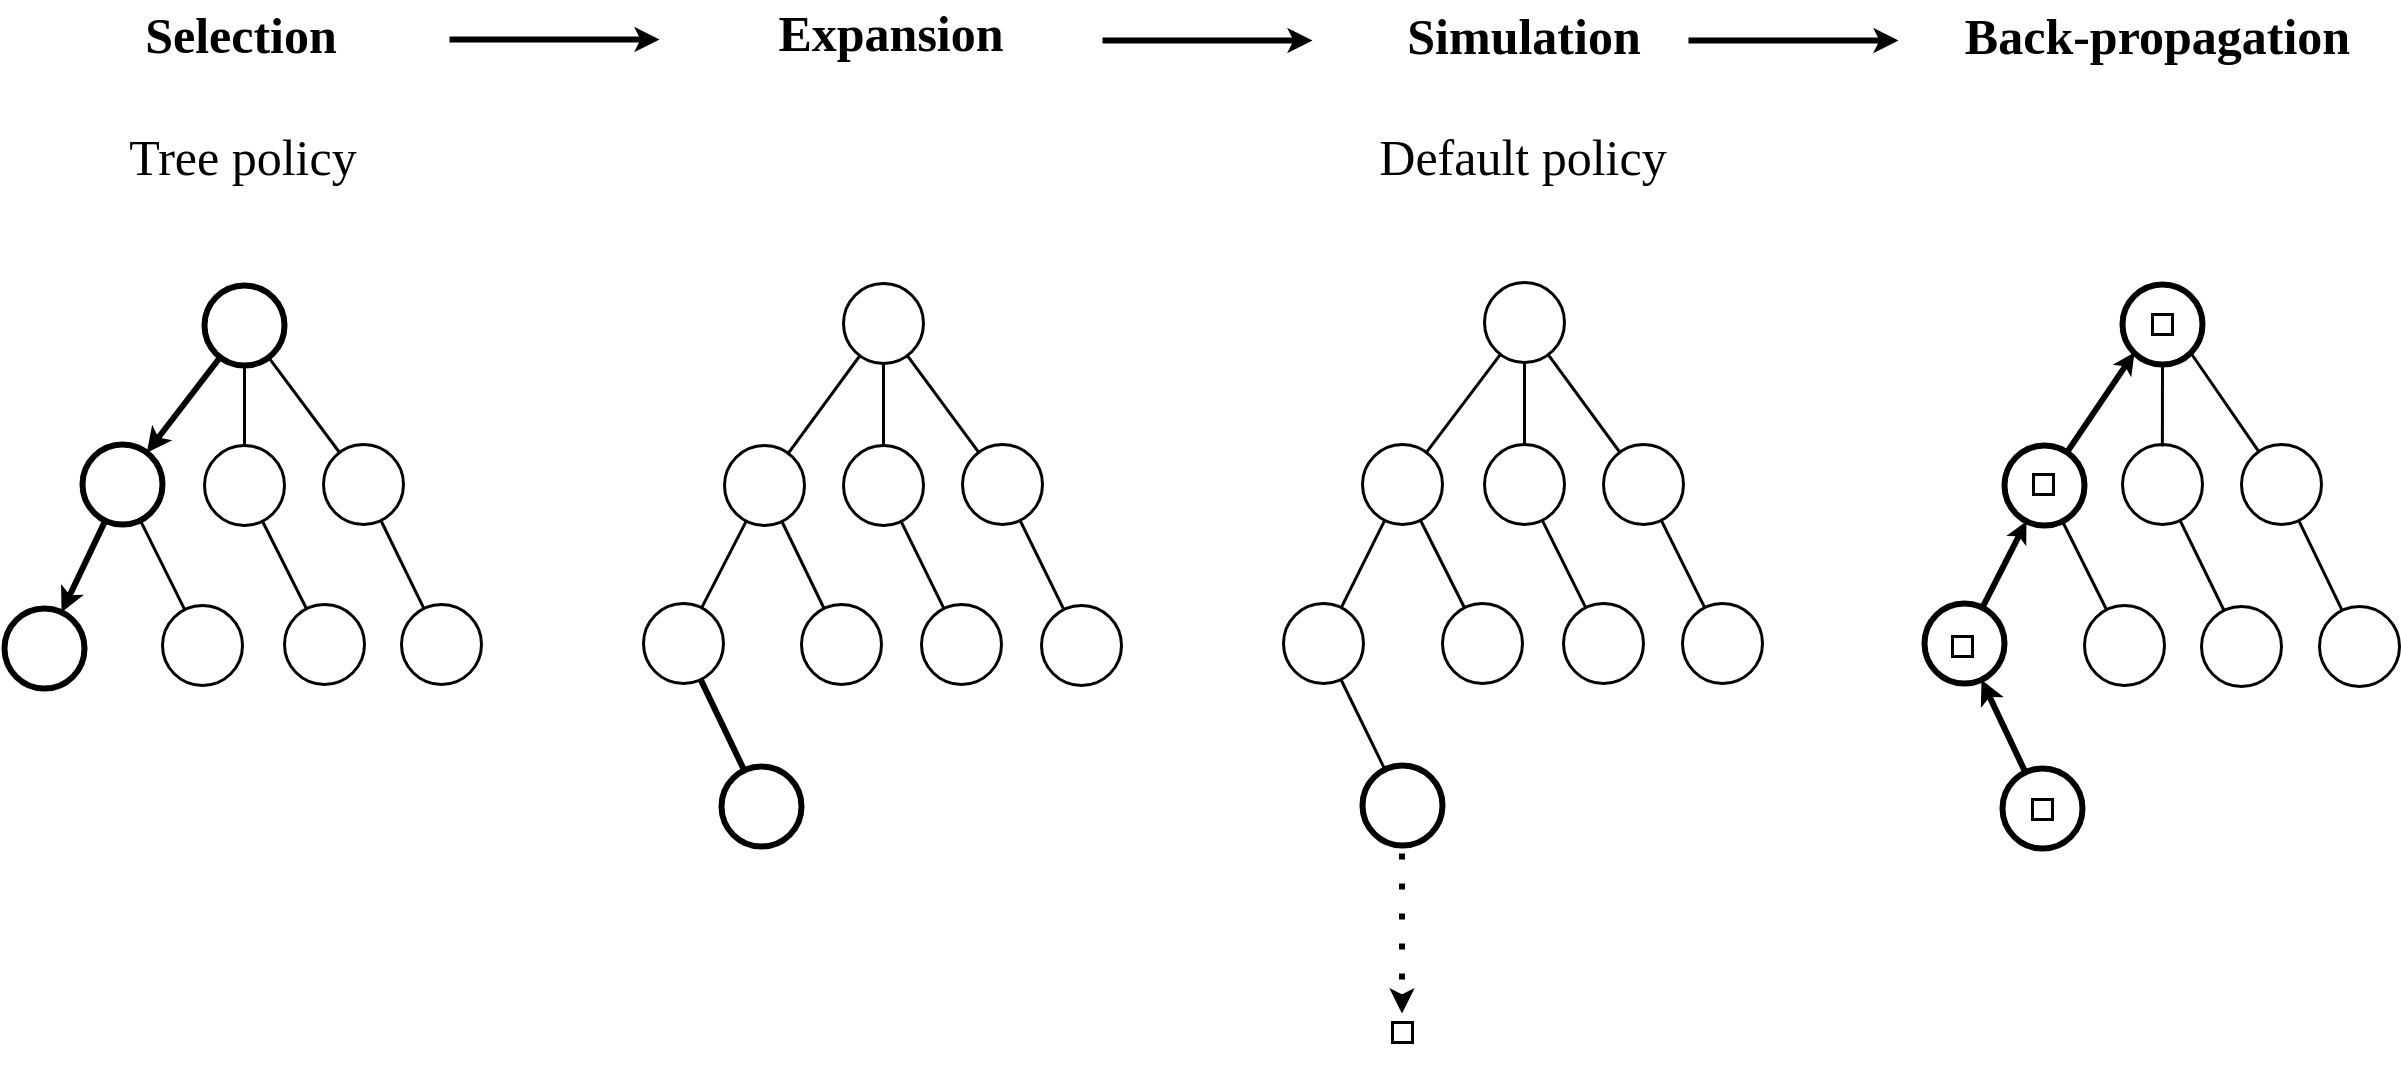
\includegraphics[width=0.9\textwidth]{Figures/mcts_plot_my2.png}
\caption{Diagram representing the four steps of UCT. Diagram adapted from~\cite{browne2012survey}.}
\label{fig:mctsplot}
\end{figure*}



\section{Methodology}\label{sec:mcts}
Many classic games like Go, Chess, and Tic Tac Toe are also combinatorial games. A popular approach to solve combinatorial games is the \textit{minimax} algorithm~\cite{knuth1975analysis}, which finds the optimal action for a player by constructing a complete search tree comprising of all possible actions alternated by each player. Minimax assumes that both parties are playing rationally, i.e., each selecting actions that maximizes their accumulated rewards or minimizing accumulated costs. Since minimax is exhaustive in nature, it does not scale well for games with a large search space such as Go. Therefore, heuristic functions to approximate the actions' values after limited search depth and/or techniques for pruning search trees~\cite{knuth1975analysis} are needed. Even with these techniques, minimax may still be infeasible or not perform well for complex search problems. 


As an alternative to minimax, \textit{Monte Carlo Tree Search} (MCTS)~\cite{coulom2006efficient,kocsis2006bandit,nguyen2014bootstrapping} is a class of heuristic search algorithms for identifying near-optimal actions without having to construct the complete search tree. It has attracted much attention in recent years due to successful application to Go-playing programs~\cite{silver2016mastering,silver2017mastering}, General Game Playing~\cite{finnsson2008simulation}, and Real-Time Strategy games~\cite{balla2009uct}. In essence, MCTS involves iteratively building a search tree at each decision state to estimate the values of the state and available actions at that state. The main idea of MCTS in improving the efficiency of search is to prioritize expanding the search trees in the direction of the most promising actions.

% In the search tree, each node represents a state, while directed edges to child nodes represent actions leading to consequent states. There exist various MCTS variations differing from each other by how the four steps are implemented and enhanced, which eventually affects how the search tree is built~\cite{nguyen2014bootstrapping}.

A draft in a normal MOBA is regarded as a combinatorial game with a branching factor at least $100$ and depth 10, since popular MOBA games such as League of Legends and DOTA 2 sport more than 100 heroes to be selected for each of the 10 picks in a draft. As the branching factor is very large in this case, which makes minimax hardly a feasible approach, we propose to apply MCTS to compute the optimal pick for the current player. 



% Each iteration consists of four steps, namely selection, expansion, simulation, and backpropagation, as shown in Figure~\ref{fig:mctsplot} and detailed in the next section.



% $\hl{MCTS has been applied in other kinds of recommendation systems.}


Specifically, we propose the use of a particular version of MCTS called \textit{Upper Confidence Bound applied to trees} (UCT)~\cite{kocsis2006bandit} for this purpose. The search tree of UCT is built iteratively, with each node representing a state and each directed edge to child nodes representing the action resulting to a next state. It starts with a root node, which, in our case, represents the draft state $s$ right before the current player is to pick the next hero. Then, the search tree is built based on the following four steps per iteration, until time or memory resource allocated is depleted:

% in which
% to add to his/her current line-up

\textbf{Selection}. In this step, the algorithm starts from the root node and traverses down the tree to reach a terminal node or an expandable node. A node is \textit{expandable} if it is a non-terminal state and has child nodes unvisited. The tree traversal is done by successively selecting child nodes, following the \textit{tree policy}, which in UCT is based on the \textit{Upper Confidence Bound} (UCB1) criterion~\cite{auer2002finite}:
    \begin{equation}
    \begin{aligned}
    \pi_{UCB1}(s) = \arg\max_a \Big\{ \bar{w} + c \sqrt{\frac{\log n(s)}{n(s, a)}} \Big\},
    \label{eqn:ucb}
    \end{aligned}
    \end{equation}
where $s$ and $a$ refer to a parent node and an action available at that node, respectively; $\bar{w}$ is the average reward received after taking $a$ at $s$; $n(s,a)$ is the number of times $a$ is sampled at $s$, and $n(s)$ is the total number of times $s$ is visited; and $c$ is the exploration term, usually chosen empirically. 

What is implied in Eqn.~\ref{eqn:ucb} is that UCT regards the choice of actions in the selection phase as multi-armed bandit problems: it focuses on \textit{exploiting} the most promising actions to expand next (controlled by $\bar{w}$), while, as a balance,  \textit{exploring} more neglected branches of the tree (controlled by $c \sqrt{\frac{\log n(s)}{n(s, a)}}$). 
    
\textbf{Expansion}. Unless the reached node from the last step is a terminal state, one of the unvisited actions is randomly sampled and applied to the node. The child node representing the resulting state is added to the tree.

\textbf{Simulation}. From the newly expanded node, the algorithm performs a roll-out until the end of the game. During the roll-out, actions are performed according to a \textit{default policy}, which by default is random sampling. Once the roll-out reaches a terminal state $s \in S_T$, $R(s)$ is calculated.

\textbf{Backpropagation}. The reward is backpropagated from the expanded node to the root node. Statistics on each node, i.e., the average reward and the number of visits, on the path are updated accordingly.

As the number of these four-step iterations increases, the algorithm expands the search tree larger and touches on more states and actions. Intuitively, the larger the search tree is, the better the value approximation of state nodes is. When the algorithm terminates, the action leading to the root's most rewarding child node, i.e., highest $\bar{w}$, is returned. The tree building process of UCT is sketched in Figure~\ref{fig:mctsplot}.

It is proven that when proper parameters are configured and rewards are bounded to the range $[0,1]$, UCT converges to minimax's optimal action at a polynomial rate as the number of iterations grows to infinity~\cite{kocsis2006bandit}. This implies that applying UCT with theoretically sufficient time and memory will eventually converge to the optimal hero for team victory. 

There are two benefits of MCTS in general that make it suitable for a hero pick recommendation system. First, state value estimation can solely rely on the backpropagation of the reward on terminal states without needing to resort to a hand authored heuristic function. This reduces the amount of domain knowledge required. Second, MCTS is an anytime algorithm, which means tree building can be interrupted when a given time or memory constraint is exceeded and estimated values based on the search tree built so far can be returned immediately. This makes it feasible for our MCTS-based method to be deployed in large-scale online matches under real-world resource constraints.

\subsection{Reward Function as a Win Rate Predictor}\label{sec:rewardfunction}
Now, we describe how the reward, i.e. the team win rate based on a hero line-up, is calculated. 

Following the previous notation, we use $w(s)$ to denote the predicted team win rate from the view of the Radiant player, based on a complete draft $s \in S_T$. This win rate can be computed by a machine learning classification model trained on a large amount of hero line-ups extracted from historical matches. During the training of such a model, the input feature vector is the completed draft as encoded in Eqn.~\ref{eqn:sifeature}; the output is a binary label indicating the observed match outcome (+1 for a win or 0 for a loss, from the view of Radiant). There are two properties making a model desirable for our task: (1) it should return the class probability, i.e., the probability of Radiant drafts winning the game, rather than just a binary prediction; and (2) it should be a non linear-based model that can capture the interrelationships between features (i.e., heroes). 


\section{Performance Evaluation}\label{ressection}
In this section, we detail the set up of our simulation-based experiments and demonstrate the effectiveness of UCT by showing that teams following our algorithm to pick heroes can form stronger hero line-ups against teams following other hero pick strategies.

\subsection{Data Collection}
We choose the DOTA2 match dataset collected between February 11, 2016 to March 2, 2016 by Semenov et al.~\cite{Semenov2016}. No major game update affecting the mechanics of the games occurred during the data collection phase. The original dataset contains five million ``Ranked All Pick'' matches, with each match containing hero line-up information and average player skill level (i.e., normal, high, and very high). To further reduce the impact introduced by different skill levels, 
we extract a subset of matches played by gamers only in the normal skill level. In total, our dataset has 3,056,596 matches, containing 111 distinct heroes. The dataset was used to train a team win rate predictor as the reward function, as well as provide a basis for our simulations.

% All used data and codes are open sourced and available online \footnote{\url{https://github.com/czxttkl/GAE}}.
\subsection{Win Rate Predictor Training}

% , while the exact number of ReLU units is determined empirically through grid search (see \hl{Experiment} section).  With the architecture designed, we expect that the neural network could capture not only the strengths of individual heroes but also interactions between them.

To prepare the data for training the team win rate predictor, each match's hero line-up is encoded as a feature vector of length 111 (Eqn.~\ref{eqn:sifeature}) while the match outcome is used as the label. 

We experiment with three classification models, Gradient Boosted Decision Tree (\textbf{GBDT})~\cite{friedman2001greedy}, Neural Network (\textbf{NN})~\cite{bishop2006pattern}, and a generalized linear model, Logistic Regression (\textbf{LR}), for the team win rate predictor. GBDT fits the logit of label probabilities with the outputs of a collection of decision trees learned using boosting~\cite{friedman2000additive}. For the NN model, we use one input layer, one hidden layer, and one output layer. The hidden layer is comprised of a number of rectified linear units (ReLU) which transform the original features non-linearly to feed the output layer. The output layer is a single neuron with the sigmoid activation function $\frac{1}{1+exp(-x)}$. 
LR models the logit of label probabilities as a linear combination of individual features without explicitly modeling the interactions among features. Therefore, although all the three models can predict the label probabilities on new data, GBDT and NN are more sophisticated and able to capture interactions among features. We also test a naive baseline model which always outputs the majority class (\textbf{MC}). In our case, it always predicts a win for Radiant because there are 53.75\%  matches in which Radiant wins. 


All hyperparameters like the number of hidden units of NN, the number of trees of GBDT and the regularization penalty of LR are determined through grid search on a 10-fold cross-validation procedure. In each fold, we split the data into the train, validate and test set in an 8:1:1 ratio. Candidate models of the same kind but with different hyperparameters are trained on the train dataset; the best hyperparameters are determined according to the classification accuracy on the validation dataset. The classification performance of the best model is measured on the test dataset.  

\begin{table}
  \caption{Performance of Team Win Rate Predictors}
  \centering
  \label{tab:auc}
  \begin{tabular}{c@{\hskip 0.5in}c@{\hskip 0.36in}c@{\hskip 0.36in}c}
    \toprule
    Model  & Accuracy & AUC  \\
    \midrule
    MC   & 0.53779        & 0.5       \\
    LR   & 0.63576        & 0.68767    \\
    GBDT & 0.64172        & 0.70142   \\
	NN   & 0.65345        & 0.71437  \\
  \bottomrule
\end{tabular}
\end{table}


We report the accuracy and area under ROC (receiver operating characteristic) curve (AUC) for each kind of model in Table~\ref{tab:auc}, averaged over 10-fold cross validation. NN achieves the best prediction performance in both accuracy and AUC. Additionally, the accuracy and AUC of NN are statistically higher than those of the other models according to a paired, two-tailed Welch's t-test with confidence level $0.05$. Thereby we decide to use NN as the reward function in our simulation experiments later. 

It is worth noting that the absolute difference between LR and NN is 1.8\% for accuracy and 0.03 for AUC, which may give a wrong impression that match outcomes are accountable by the sum of individual heroes' effects and hero interactions are not as important as we want to emphasize. We propose a possible explanation for this phenomenon, that players already tried hard to build closely competitive hero line-ups in the collected matches such that good or bad hero interactions are hard to stand out. If we train the models with additional matches in which players (or human-like AI bots) are forced to play random heroes, NN may have a larger edge over LR. We will investigate such an issue in the future.




\subsection{Simulation Setup}
We design four strategies for hero pick recommendation and test their effectiveness in terms of team victory. For every pair of strategies, we conduct 1000 simulations: in each simulation, two teams participate in the drafting process, with each team adopting one of the two strategies. At the end of each draft, we collect the predicted win rate as measure of strength of the built hero line-ups. Finally, we will report the mean of the predicted win rates over the 1000 drafts for each pair of strategies. The procedure of one simulation is summarized in Algorithm~\ref{alg:sim_match}.

\begin{algorithm}
    \SetKwInOut{Input}{Input}
    \SetKwInOut{Output}{Output}
    \SetKwFunction{Armijo}{armijo} 
    \Input{team1, team2, win rate predictor $\mathcal{M}$}
    \Output{$w(s)$}
    \BlankLine
    Initialize a new draft $s:= s_{0}$ 
    \BlankLine
    \While{$s \not\in S_T$} {
    team = $\rho(s)$
    
    \uIf{$s$ equal to $s_0$}{
    
        $a$ = weighted\_sample\_hero()
        
    }
    \Else{
    
        $a$ = team.recommend\_hero($s$)
        
    }
    
    
    $s = f(s,a)$
    }
    
    $w(s)$:= predicted by $\mathcal{M}$ with input $s$
    \caption{Simulation of one match}
    \label{alg:sim_match}
\end{algorithm}

\begin{table*}
  \caption{Mean predicted win rate of $UCT_{n, 1}$ (row) vs. $UCT_{n, c}$ (column). Numbers are from the view of the row strategy. Bold cells indicate the best value of $c$ for $UCT_{n,c}$ for each $n$, as they force $UCT_{n,1}$ have the lowest win rate.}
  \label{tab:param_set}
  \centering
  \begin{tabular}{ccccccccc}
    \toprule
      & $UCT_{n,2^{-6}}$ & $UCT_{n, 2^{-5}}$ & $UCT_{n, 2^{-4}}$ & $UCT_{n, 2^{-3}}$ & $UCT_{n, 2^{-2}}$ & $UCT_{n, 2^{-1}}$ & $UCT_{n, 2^0}$ & $UCT_{n, 2^1}$\\
    \midrule
    $UCT_{100, 1}$ & 0.5 & 0.5 & 0.5 & 0.5 & 0.5 & 0.5 & 0.5 & 0.5\\
    $UCT_{200, 1}$ & 0.459 & \textbf{0.435} & 0.442 & 0.444 & 0.447 & 0.464 & 0.5 & 0.540 \\
    $UCT_{400, 1}$ & 0.497 & 0.476 & 0.469 & 0.469 & \textbf{0.457} & 0.469 & 0.5 & 0.534 \\
    $UCT_{800, 1}$ & 0.561 & 0.544 & 0.527 & 0.509 & 0.488 & \textbf{0.485} & 0.5 & 0.525 \\
    $UCT_{1600, 1}$ & 0.606 & 0.577 & 0.563 & 0.545 & 0.510 & \textbf{0.492} & 0.5 & 0.516 \\
  \bottomrule
\end{tabular}
\end{table*}


The four experimented strategies include:
\begin{itemize}
\item \textbf{UCT}: this strategy is what we propose in Section~\ref{sec:mcts}. We will use $UCT_{n,c}$ to denote a specific UCT version with $n$ iterations allowed and an exploration term $c$. 
\item \textbf{Association Rules (AR)}: this strategy was proposed by Hanke and Chaimowicz~\cite{hanke2017reco}. Two sets of association rules, namely ``ally rules'' and ``enemy rules'', are extracted from the collected matches. Ally rules and enemy rules represent hero subsets that appear frequently in the same winning team or in the opposite team, respectively. At each turn, the strategy looks for the extracted association rules containing both the heroes picked already and the heroes not picked yet. Those not picked yet will be selectively added to a candidate pool, from which the recommended hero will be uniformly sampled. In our implementation, we adopt the best criteria claimed by the authors: association rules are mined with $0.01\%$ minimum support, and the metrics for selectively adding heroes to the candidate pool are ``win rate'' and ``confidence'' for ally rules and enemy rules, respectively. Readers can refer to the original paper~\cite{hanke2017reco} for more details on the approach. 
\item \textbf{Highest Win Rate (HWR)}: each time, pick the hero not selected yet with the highest win rate, based on frequency counts on our dataset. 
\item \textbf{Random (RD)}: each time, uniformly sample a hero not yet selected. 
\end{itemize}

We do not implement the strategy based on sequence prediction models as proposed by Summerville et al.~\cite{summerville2017reco} because their model requires training on hero pick sequences, which are not readily available in our dataset. In fact, hero pick sequences are not currently downloadable from the official APIs provided by the game and need to resort to third-party organizations. We would implement the strategy in the future should we have access to such data of hero pick sequences.

Some additional implementation details are as follows. For each simulated draft, regardless of the strategy adopted, the first hero is sampled following the probability distribution reflecting how frequently each hero is picked in our dataset. This helps our experiments cover more possible scenarios. To ensure fairness when comparing pairs of strategies, among the 1000 simulations, each strategy is set to start first for half of the simulations. A shared random seed is set for each 500-simulations, to make sure that randomness is the same for both strategies. All strategies follow the rule that no hero can be picked twice. All experiments are conducted on a PC with an Intel i7-3632QM 2.20GHz CPU. The relevant code will be made available upon publication at \url{https://github.com/czxttkl/DraftArtist}.

\subsection{Parameter Search for UCT}

We first run simulations to determine the exploration term $c$ for the UCT strategy. We choose $UCT_{n, 1}$ as benchmarks (i.e., UCT with the exploration term ${c=1}$), where ${n=\{100, 200, 400, 800, 1600\}}$. For each $UCT_{n,1}$, we then create multiple $UCT_{n, c}$ strategies to play with, with $c$ ranging from $2^{-6}$ to $2$ at a scaling rate of $2$.

The results are shown in Table~\ref{tab:param_set}. Tuning $c$ is not helpful when UCT is only allowed with 100 iterations. This is because $c$ controls the exploration strength for tree node selection in the \textit{selection} step, which never kicks off within 100 iterations due to the large number of available actions\footnote{We have 111 distinct heroes and 10 turns in a draft, which means applying UCT at any turn will start from a root state with more than 100 possible child nodes (actions) to expand. Since one iteration only expands one new child node, after 100 iterations, the root node is still expandable. Therefore, no selection step will happen. }. We can infer that the best value of $c$ to couple with ${n=\{200, 400, 800, 1600\}}$ is $2^{-5}$, $2^{-2}$, $2^{-1}$ and $2^{-1}$, respectively, because they force $UCT_{n, 1}$ to have the lowest win rate (indicated by the bold cells in Table~\ref{tab:param_set}). Note that there is a general trend that the best $c$ increases as $n$ increases.

% $c$ is not effective in $UCT_{100, c}$ because no selection phase takes place. The selection phase only happens after the root node is no longer expandable. However, the root node will always be expandable within 100 simulations because there are more than 100 heroes that can be picked at any turn and the root node expands only one child node per iteration. 


\begin{table*}
  \caption{Mean predicted win rate of row strategy  vs. column strategy. Simulations are based on the drafting rules of match mode ``All Ranked''. Numbers are from the view of the row strategy. The strategies are sorted in ascending order by their strengths, from top to bottom, and from left to right. Win rates symmetric to diagonal and always sum to one, thus half of them are omitted.}
  \label{tab:mcts}
  \centering
  \begin{tabular}{ccccccccc}
    \toprule
      & $RD$ & $AR$ & $UCT_{100, 1}$ & $UCT_{200, 2^{-5}}$ & $HWR$  & $UCT_{400, 2^{-2}}$ & $UCT_{800, 2^{-1}}$ & $UCT_{1600, 2^{-1}}$ \\
    \midrule
    $RD$ & 0.5 &  &  &  &  &  &  &  \\
    $AR$ & 0.682 & 0.5 &  &  &  &  &  & \\
    $UCT_{100, 1}$ & 0.783 & 0.663 & 0.5 & & &  &  \\
    $UCT_{200, 2^{-5}}$ & 0.897 & 0.833 & 0.712 & 0.5 & & & \\
    $HWR$ & 0.883 & 0.846 & 0.715 & 0.516 & 0.5 \\
    $UCT_{400, 2^{-2}}$ & 0.920 & 0.863 & 0.763 & 0.568 & 0.556 & 0.5   \\
    $UCT_{800, 2^{-1}}$ & 0.928 & 0.878  & 0.776 &  0.591 & 0.593 & 0.524 & 0.5 &  \\
$UCT_{1600, 2^{-1}}$ & 0.930 & 0.880  & 0.787 & 0.606 & 0.611 & 0.539 & 0.513 & 0.5 \\
  \bottomrule
\end{tabular}
\end{table*}

\begin{table*}
  \caption{Average wall time per pick of different strategies (unit: millisecond, match mode: All Ranked).}
  \label{tab:mcts_time}
  \centering
  \begin{tabular}{ccccccccc}
    \toprule
      $RD$ & $AR$ & $UCT_{100, 1}$ & $UCT_{200, 2^{-5}}$ & $HWR$  & $UCT_{400, 2^{-2}}$ & $UCT_{800, 2^{-1}}$ & $UCT_{1600, 2^{-1}}$ \\
    \midrule
     0.02 & 11 & 43 & 96 & 0.1 & 281 & 562 & 1120 \\
    \bottomrule
\end{tabular}
\end{table*}

\begin{table*}
  \caption{Mean predicted win rate of row strategy  vs. column strategy. Simulations are based on the drafting rules of match mode ``Captain Mode''. The table can be viewed in a similar way as Table~\ref{tab:mcts}.}
  \label{tab:mcts_captain_mode}
  \centering
  \begin{tabular}{ccccccccc}
    \toprule
      & $RD$ & $AR$ & $UCT_{100, 2^{-5}}$ & $UCT_{200, 2^{-5}}$ & $HWR$  & $UCT_{400, 2^{-2}}$ & $UCT_{800, 2^{-1}}$ & $UCT_{1600, 2^{-1}}$ \\
    \midrule
    $RD$ & 0.5 &  &  &  &  &  &  &  \\
    $AR$ & 0.693 & 0.5 &  &  &  &  &  & \\
    $UCT_{100, 2^{-5}}$ & 0.817 & 0.686 & 0.5 & & &  &  \\
    $UCT_{200, 2^{-5}}$ & 0.91 & 0.851 & 0.712 & 0.5 & & & \\
    $HWR$ & 0.876 & 0.788 & 0.694  & 0.508 & 0.5 \\
    $UCT_{400, 2^{-2}}$ & 0.929 & 0.886 & 0.770 & 0.574 & 0.570 &  0.5  \\
    $UCT_{800, 2^{-1}}$ & 0.941 & 0.896 & 0.788 & 0.598 & 0.607 & 0.536 & 0.5 &  \\
$UCT_{1600, 2^{-1}}$ & 0.942 & 0.903 & 0.797 & 0.620 & 0.627 & 0.552 & 0.519 &  0.5 \\
  \bottomrule
\end{tabular}
\end{table*}


\subsection{Simulation Results}
Based on the results from the parameter search, we finally choose a list of strategies to compare with each other: $RD$, $AR$, $HWR$, $UCT_{100, 1}$, $UCT_{200, 2^{-5}}$, $UCT_{400, 2^{-2}}$, $UCT_{800, 2^{-1}}$, and $UCT_{1600, 2^{-1}}$. The simulation results are summarized in Table~\ref{tab:mcts}, in which each cell contains the mean predicted win rate of the strategy displayed on the respective row. 

We define the strength of a strategy as the number of strategies it can defeat with more than $50\%$ win rate. Therefore, the weakest to strongest strategies are: $RD$, $AR$, $UCT_{100, 1}$, $UCT_{200, 2^{-5}}$, $HWR$, $UCT_{400, 2^{-2}}$, $UCT_{800, 2^{-1}}$, and $UCT_{1600, 2^{-1}}$. Given a sufficient number of iterations ($\geq400$), UCT strategies can outperform all non-UCT strategies, which proves the effectiveness of our proposed algorithm. There is a general trend that UCT improves the win rate as the number of iterations increases. Specifically, $UCT_{1600, 2^{-1}}$ can beat $HWR$ with a 61.1\% win rate, highest among the other UCT-based strategies with fewer iterations. However, we can observe the phenomenon of diminishing gain as the number of iterations exceeds a certain threshold: $UCT_{1600, 2^{-1}}$ has a $51.3\%$ win rate against $UCT_{800, 2^{-1}}$, only marginally better than $50\%$ but with double the number of iterations.

Among non-UCT strategies, the $HWR$ strategy that always picks the highest win rate hero achieves the best performance, which can defeat UCT with 200 iterations with a $51.6\%$ win rate. However, $HWR$ cannot prevail over UCT strategies that are allowed more than 200 iterations. $AR$ adopted from~\cite{hanke2017reco} defeats $RD$ with $68.2\%$ win rate for our implementation, while the original authors reported a $76.4\%$ win rate against $RD$. The discrepancy may be due to different datasets being used to mine association rules and train the win rate predictor.

To show the efficiency of different strategies, we report the average wall time (i.e. real elapsed time) needed per pick in Table~\ref{tab:mcts_time}. The time is recorded excluding the first pick, since it is based on weighted random sampling. UCT-based strategies take 1.12 seconds or less per pick, which is a small fraction of the 25 second time limit per pick for human players in real matches~\cite{dotapickorder}. This demonstrates the feasibility of applying the UCT-based hero recommendation system online in large scale and real time.


\begin{figure*}
\centering
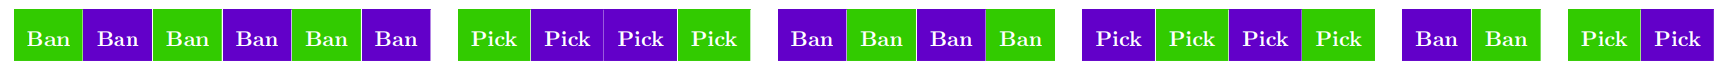
\includegraphics[width=1\textwidth]{Figures/pickorder_captain_mode_my.png}
\caption{Drafting order in match mode "Captain Mode" in DOTA 2. The green and purple cells represent the turns of two different teams (i.e., Radiant and Dire), assuming the green team starts first. Diagram is adapted from~\cite{dotapickorder} and best viewed in color.}
\label{fig:pickorder_captain_mode}
\end{figure*}

\subsection{Extension to Other Match Modes}\label{sec:draftart_extension}
What we have focused on so far in this paper is based on the drafting rules of match mode \textit{All Ranked} in DOTA 2. However, our MCTS-based algorithm is not limited solely to this mode and can be adapted to other modes, whereby additional drafting rules and mechanics are deployed. In this section, we detail how our algorithm can be extended to another popular match mode called \textit{Captain Mode} to demonstrate our algorithm's generality. 

During the drafting process in Captain Mode matches, there is another type of action, called \textit{hero banning}, that players can take besides hero pick. In the turns of banning, a team can designate certain heroes to be prohibited from selection by either team. The drafting order is represented in Figure~\ref{fig:pickorder_captain_mode}: two teams first alternate to ban three heroes, then alternate to pick two heroes, then alternate to ban two heroes, and so on. As the result, the drafting is 22 steps long, instead of just 10 as in the case of \textit{All Ranked}. The interleaving nature between bans and picks adds another level of complexity to the drafting, as players need to consider more possible strategies to prevent opponents from selecting their desired heroes. 

Despite being more complex, the drafting in Captain Mode matches can be formulated as a combinatorial game similar to that in All Ranked matches but with a few minor adjustments:

\begin{itemize}
    \item The components of a game state $s$ can take an additional value of a special symbol $\Xi$ denoting corresponding banned heroes, i.e.,:
\begin{equation}
s_{i}=
\begin{cases}
  1, & \text{hero } i \text{ picked by Radiant} \\
  -1, & \text{hero } i \text{ picked by Dire} \\
  \Xi, & \text{hero }i \text{ banned} \\
  0, & \text{otherwise}
\end{cases}
\label{eqn:sifeature}
\end{equation}

The terminal state set $S_T$ will also change accordingly. A terminal state $s \in S_T$ include five ones, five negative ones, and 12 special symbol $\Xi$.

    \item An action can be either a ban or a pick. If it is a ban, $f(s,a)$ changes a zero component of a non-terminal state $s \in S \setminus S_T$ to $\Xi$. 
    \item The turn function $\rho$ will also be updated to reflect the drafting order in Figure~\ref{fig:pickorder_captain_mode}.
    \item When a terminal state $s \in S_T$ is fed into the reward function $R(s)$, its components of $\Xi$ will be treated as zeroes.
\end{itemize}

Given the above formulation of the Captain Mode drafting, in the form of a combinatorial game, the UCT algorithm can be applied directly in the same way as described in Section~\ref{sec:mcts}. Within the drafting rules of Captain Mode matches, we conduct the same simulation-based experiments to compare UCT with the baselines $RD$, $AR$ and $HWR$. When taking the banning action, $AR$ is executed from the perspective of the opponent - identifying candidate heroes to ban as if the opponent is to pick; $HWR$ always chooses among the available heroes with the highest win rate for both the pick and ban actions. Regarding other implementation details, the selection frequency-weighted sampling is executed for the first hero to ban rather than the first hero to pick. $c$ becomes effective in $UCT_{100, c}$, since the simulation step may kick off after the starting root node is no longer expandable. We find the best $c$ to match with ${n=100}$ is $2^{-5}$, while the best $c$ values to couple with other ${n=\{200, 400, 800, 1600\}}$ remain the same as in All Ranked experiments.

The evaluation results are shown in Table~\ref{tab:mcts_captain_mode}. First, we observe that the strength order of the tested strategies remains the same, with $RD$ being the weakest and $UCT_{1600, 2^{-1}}$ being the strongest. Second, the win rate of UCT strategies against non-UCT strategies usually sees a 1-3\%  improvement in absolute value compared to the counterparts in All Ranked experiments. For example, $UCT_{1600, 2^{-1}}$ has a 62.7\% win rate against $HWR$ in Captain Mode, which is larger than the win rate $UCT_{1600, 2^{-1}}$ has against $HWR$ in All Ranked (61.1\%). This highlights the advantage of employing simulation-based approaches such as MCTS: that the advanced planning brought by the MCTS algorithm could further widen its gap over baseline methods in more sophisticated settings.

We also observed a negligible change in the average wall time needed per pick in Captain Mode-based simulations, as compared to All Ranked (Table~\ref{tab:mcts_time}), so we do not report it here. This implies that the overhead incurred by the deeper search in UCT is relatively smaller than that in other components, such as computing the reward function. 


\section{Summary}

In this chapter, we attempt to answer \hyperref[rq1]{\textbf{R.Q.~1}} in the team-vs-team setting by proposing a recommendation system, DraftArtist, that can effectively and efficiently search for winning-effective characters which are  approximately optimal for team victory based on Monte Carlo Tree Search. We design and conduct simulation-based experiments based on two kinds of drafting rules, confirming that MCTS-based recommendations can lead to stronger hero line-ups in terms of predicted team win rates, as compared to other baselines. The proposed system can be easily extended to other types of in-game elements in the team-vs-team setting where interactive selection of in-game elements by other players is influential to the player's choice. 
% One limitation of this work is that we do not consider player-specific information, such as player skills in their selected heroes, when recommending heroes. It is possible that a hero recommended by our algorithm, which is based solely on the current hero line-up, may be poorly played by a player who is not familiar with it. Our algorithm can be extended to integrate player skills, by augmenting the game state with player information and training a more advanced win rate predictor as the reward function which takes as input both hero picks and player-specific information. This limitation could be addressed when we have access to needed player-specific data.

% Another limitation is that we have only conducted experiments based on matches played by normally skilled players. In our future research, we would like to extend similar experiments onto matches of more kinds of skill brackets and investigate whether and how player skills would affect the performance of our system. 


% There are some other promising future directions that we can pursue next. First, were hero pick sequences from real match data available, we would integrate them as prior information to improve the tree policy and default policy in MCTS, thereby improving capabilities to build search trees more effectively and efficiently~\cite{gelly2007combining,chaslot2009adding}. Second, we would also like to investigate how our recommendation system can be customized to account for additional drafting rules and extended to other real-world scenarios such as player drafting in sports~\cite{staw1995sunk}. Lastly, we would like to study how to train more accurate win rate predictor models which can effectively discover more profound interrelationships among heroes.  
 
\chapter{Engagement Optimized Matchmaking} 

\label{chapter:eomm} 

\section{Introduction}\label{sec:eomm_intro}
This chapter aims to answer \hyperref[rq2]{\textbf{R.S.Q.~2}}, which we reiterate here:

\begin{equation}
  \tag{R.S.Q.~2}\label{rq2}
  \parbox{\dimexpr\linewidth-4em}{%
    \strut
    How can we design systems working in the pre-match stage which recommend in-game elements for improving player engagement through data-driven approaches?
    \strut
  }
\end{equation}

Techniques that we studied in the previous two chapters give players a better chance of winning. Guided by theories such as Self-Determination Theory and Flow, such techniques are useful to help incompetent players regain competence and enter cognitive states like flow, which we believe will then lead to engagement. In this sense, techniques from the previous two chapters are categorized as indirect and theory-driven methods.

In another perspective, \hyperref[rq2]{\textbf{R.S.Q.~2}} takes a more direct stab by investigating data-driven methods to influence player engagement using in-game element recommendations. Data-driven approaches determine recommendations purely based on analysis and interpretation from past player data, without the need to rely on psychological and sociological theories as in~\hyperref[rq1]{\textbf{R.S.Q.~1}}.
To achieve this goal, the system features the abilities to predict the change of player engagement resulting from each in-game element and efficiently search for the in-game element leading to the optimal player engagement, where player engagement is often modeled and predicted quantitatively based on machine learning models. Bypassing the intermediate links between winning-effectiveness and player competence, and between player competence and engagement, \hyperref[rq2]{\textbf{R.S.Q.~2}} offers an alternative approach to improve player engagement.



% Player-versus-Player (PvP) is a mode of video game in which multiple players directly engage in competition or combat. PvP games, which cover many popular genres, such as multiplayer online battle arena (MOBA), first-person shooting (FPS), and e-Sports, have increased worldwide popularity in recent years. For example, \textit{League of Legends}, one of the most played MOBA games, has 90 million summoner names registered, 27 million unique daily players and 7.5 million concurrent users~\cite{fanbase,27million}. As data released by~\cite{superdata} shows, e-Sports is estimated to have 188 million viewership and 748 million dollar worth market in 2015 and the numbers are expected to grow continuously.

We answer \hyperref[rq2]{\textbf{R.S.Q.~2}} with an opponent recommendation system. Opponent recommendation is also known as ``matchmaking''~\citep{medler2011using}. Since the term matchmaking has been used more frequently in existing literature, we will use matchmaking and opponent recommendation interchangeably in the rest of this chapter. In this work, we specifically develop an opponent recommendation system for Player-vs-Player (PvP) games, a subset of match-based games described in Chapter~\ref{chapter:intro}. In this case, players themselves are the subject of recommendation and the goal is to connect players to form  PvP matches. Back in Chapter~\ref{chapter:intro}, we discussed that participants can be either human players or AI bots in match-based games, unless those as the recipients of our recommendations should be human players. PvP games allow only human players, and in the  problem we study here, every player is the recipient as well as the subject of recommendation. 

We first look at the definition of opponent recommendation (or matchmaking). Most existing works have restricted the definition of matchmaking as players are exactly divided and matched. In our work, we also adopt this definition. This definition constrains the search space, since no player is allowed to be matched into multiple matches. For example, matchmaking applied in a one-vs-one PvP game will pair each player to exactly one other player. 

% not very relevant
% Under this definition, matchmaking results still means ``recommendation'' to players because they have the ability to aca player is not completely unable to choose the recommended players; we observe many modern games allow players to quit a matchmaked line-up before the match officially starts.

In practice, a matchmaking system often operates on several constraints, including physical and technical. For example, the system may be constrained by players' geo-location and network latency because connection lags caused by long geographical distance between multiple players may incur interrupted play experience. Thus, the system may prioritize to matchmake players from close regions.

Beyond physical and technical constraints, the strategy a fair amount of matchmaking systems employ is \emph{creating fair games}. This goal is inspired by the theories such as Self-Determination Theory (SDT)~\citep{ryan2000self} and Flow~\citep{flow1990psychology}, as we introduced in Section~\ref{sec:related_theory_eng}, which propose that one component of player engagement is from challenges matching with skills. This means that these matchmaking systems are often developed with the goal of matching closely skilled players to create competitive but fair games, where appropriately challenged players are matched up. 

In order to deliver on creating fair matches, numerous skill models have been proposed, such as Elo~\citep{elo1978rating}, Glicko~\citep{glickman1999parameter} and TrueSkill~\citep{herbrich:trueskill}. The main idea of skill models is to estimate player skills in formal mathematical frameworks such that outcomes between players can be predicted numerically. Based on numerical outcome prediction, matchmaking systems can then divide players into groups which are projected to have balanced outcome probabilities (as close as possible to 50\% win rates). Skill models will be reviewed in more details in Section~\ref{sec:skill_review}.

In this chapter we challenge the goal of \textit{always} creating fairly matched games because such a goal was developed based on theories  but is worthy of deep investigation in the lens of a data-driven approach, in which player engagement is examined individually depending on personal experience. Let's review some hypothetical examples where such assumptions break. Consider a cautious player who cares about protecting his rank among friends, and a risk-taker who enjoys difficult matches. Pairing these players with similarly skilled opponents will have different effects: the cautious player may be frustrated with just a 50\% win rate because his rank cannot improve further, while the risk-taker may feel bored even at a 50\% win rate. Additionally, the experience the player had with the game in the previous matches, such as how many matches he won before or lost, can affect their expectations and their experience as well as their performance. 

To give a more concrete example, see Table~\ref{tab:churnrate}, which displays data from a popular PvP game developed by Electronic Arts, Inc. Please note that we cannot disclose the name of the game in this dissertation due to contractual limitations. In the table, we show an example of how win/loss in previous games can affect players' engagement, in this case defined in terms of 7-day churn risk. It measures the likelihood of one player stopping playing the game in the next 7 days, or from a population-wise perspective, the ratio of a group of players who stop playing within the next 7 days time after a match. We can see from Table~\ref{tab:churnrate} that the churn risk varies drastically based on players' recent match outcomes, thus raising the need to cater player engagement by a data-driven approach. 

Given this information, we then devised a new matchmaking framework, called Engagement Optimized Matchmaking (EOMM). In this system, we rely on two key insights: (1) the effectiveness of matchmaking needs to be measured quantitatively; and (2) matchmaking should depend on dynamic and individual \emph{player states}. We therefore formulated matchmaking into an optimization problem, where we maximized the overall player engagement, or equivalently, minimized the overall player disengagement through pairing two players. Player disengagement is a chosen quantitative metric at the disposal of practitioners, for example, \emph{churn risk} within a period of time, such as a week. For the illustration purpose, we also use churn risk as the player disengagement metric in this chapter. Next, we modeled all players to be matched as a complete graph, where each player is a node, and an edge between two players is their sum churn risk, if paired. The churn risk depends on individual player states at the moment of matchmaking, which include but not limit to player skills. We then developed an optimization system that solves a \emph{minimum weight perfect matching} (MWPM) problem finding non-overlapping pairs with the minimal sum of edge weights on a complete graph. In order to implement and test this system, we developed a simulated system based on real data of a popular game made by Electronic Arts,\! Inc.\! (EA). As we shall show in the results section, the system showed improvement in enhancing player engagement as compared to equal-skill based and other matchmaking methods. At the time of writing, we were unable to test our system in production due to time constraint and would leave that for future work.

% Moreover, we can even change the objective function to other data-driven metrics of player engagement, such as play time, retention, or spending. EOMM allows one to easily plug in different types of predictive models to achieve the optimization.

% unrelated
% Since EOMM was developed based on a constraint optimization system, it presents a solid theoretical framework for matchmaking analysis, where we can encode different constraints by which to match make. For example, using this system we can encode matchmaking based on skill as a special case of EOMM. The generic EOMM instead proves to be optimal across a wide range of  contexts.

EOMM is both flexible and computationally feasible. The final system is composed of three components: a skill model, an engagement (e.g., churn) prediction model and a graph matching model. All can be efficiently implemented and independently upgraded. The disengagement metric in the engagement prediction model can be selected differently for various interests, e.g., in-game time, or even spending. 

% In sum, this paper contains the following contributions. First, we propose an engagement optimized matchmaking framework, i.e., EOMM, which solves matchmaking as an optimization problem of maximizing the overall player engagement. Second, we provide theoretical analysis about the optimality of EOMM and the conditions of the applicability of existing matchmaking methods. Last, we build a simulated system using real game data to show significant advantages of EOMM in retaining players over the existing matchmaking methods.

The rest of this chapter is organized as follows. After reviewing the related work, we will present the formulation of matchmaking as an optimization problem on a graph. Then we describe theoretical findings comparing EOMM and other matchmaking methods. We then show the case study applying EOMM on real data. Finally, we will conclude with a discussion of the results and future directions.


\begin{table}[tb]
\centering
\caption{
An example of the impact of player states on their engagement. Data is from a popular PvP game made by EA. Average churn risks vary drastically upon players' recent three match outcomes (\emph{(W)in}, \emph{(L)ose} or \emph{(D)raw}). Churn risk is measured by the ratio of the players who stop playing within a period time (7 days in this table) after a match. The churn risk of some states with repeated losses (5.1\%) is almost twice as much as those of other "safer" states (2.6\%-2.7\%).
} \label{tab:churnrate}
\vspace{2mm}
\begin{tabular}{|c|c|}
\hline
Last 3 Outcomes & Churn Risk                      \\ \hline
DLW $|$ LLW $|$ LDW $|$ DDD      &  2.6\% - 2.7\%        \\
... & ...  \\
WWW   &  3.7\% \\
... & ... \\
DLL $|$ LWL $|$ LDL  &  4.6\% - 4.7\%  \\
WWL & 4.9\% \\
LLL & 5.1\% \\
\hline
\end{tabular}
\end{table}


\section{Related Work}\label{sec:review}

In this chapter, we introduce three relevant fields, namely skill modeling, player engagement prediction, and graph matching. Each field is actually one critical component of our proposed matchmaking framework.

% [please add something here to discuss why we are looking at skill modeling, etc.. ]

\subsection{Skill Modeling}\label{sec:skill_review}
Skill modeling aims to model player skills in mathematical frameworks and gives numeric  prediction on match outcomes between players. Skill models can facilitate EOMM in the decision of player assignment. We would like also to compare our work to fairness-based matchmaking systems that use skill models.  Therefore, we will review the models proposed for skill modeling here. 

% The motivation behind skill rating is to rank players and to enable skill-based matchmaking. 

Skill modeling has had a long history. Dating back to 1952, the \textit{Bradley-Terry model} \citep{bradley1952rank} was developed to deal with repeated pairwise comparisons among a group of subjects. In the Bradley-Terry model, a player $i$ is assumed to have a fixed, positive skill scalar, $r_i$, and the winning probability of player $i$ against player $j$ is the ratio of player $i$'s skill in the sum of skills of both players. In its original form, the Bradley-Terry model estimates player skills only after observing all pairwise comparisons. While feasible for small groups of players, requiring $O(n^2)$ matches is prohibitive for large player pools. One can show that the Bradley-Terry model is equivalent to a logistic regression model \citep{agresti2011categorical} in which each coefficient $w_i$ corresponds to $\log(r_i)$.

The \textit{Elo system} \citep{elo1978rating} addresses the relative skill ratings in player-versus-player games, such as chess, by proposing a probabilistic model. Elo captures player performance, $p_i$, as a random variable following a one dimension Gaussian distribution with a mean, $r_i$, and a fixed variance, $\beta^2$, shared by all players. In the Elo system, $r_i$ is updated depending on the extent of agreement between expected outcomes and real outcomes. For example, a player beating a higher skilled player yields a large update in adjusting their skill means closer. Unlike the original Bradley-Terry model, in this model $r_i$ can be updated at an ongoing basis, i.e., as soon as after every match of player $i$.

The \textit{Glicko system} \citep{glickman1999parameter}, a Bayesian ranking rating system, was later introduced. Besides mean player skill, $r_i$, it also models the belief about a player's skill as $RD_i$ (rating deviation). As they play more games, the belief about their skills become stronger hence $RD_i$ decreases. However, $RD_i$ increases when a player ceases to play for long time. To achieve high efficiency, Glicko uses an approximation Bayesian algorithm to update $r_i$ and $RD_i$.

Neither the Bradley-Terry model, the Elo system or the Glicko system was initially applicable to team-oriented games until some researchers looked into how to generalize these models for use in team games ~\citep{herbrich:trueskill,huang2004generalized,menke2008bradley}. \textit{TrueSkill system}~\citep{herbrich:trueskill} extends the Elo system to games with flexible numbers of players and teams. TrueSkill assumes that the outcome of a team-vs-team match results from the discrepancy of team performance; team performance is the sum of individual performances, whereas an individual performance is governed by his or her skill rating. Given TrueSkill's form in a generative model, skill ratings can be computed by Bayesian inference using a specific technique named Expectation Propagation~\citep{minka2001expectation}. \textcite{huang2004generalized} derived analytic update rules that are easy to interpret and implement using a Bayesian approximation
method. Their model works for games with multiple teams and multiple players by treating a $k$-team match as several two-team matches. \textcite{menke2008bradley} proposed to use Artificial Neural Network (ANN) for extending the Bradley-Terry model to team-based games.

Researchers have proposed more advanced skill models to overcome  limitations of aforementioned skill models. First, the aforementioned models only abstract player skills into a single dimension but in fact many games require skills from multiple facets. To improve upon that, the works by~\textcite{chen2016modeling} and~\textcite{stanescu2011rating} model player skills in multi-dimensions, such as offensive and defensive abilities. \textcite{Delalleau2012} proposed a neural network based skill model which learns multi-dimensional latent skill embeddings of players and is claimed to outperform TrueSkill in a team based game. Second, it is desirable to incorporate more domain-specific information that might help estimate player skills more accurately therefore researchers have devised skill models for specific game genres. For example,  \textcite{di2009skill}'s skill model for chess integrate move and position evaluation. \textcite{zhengxing2016player} and \textcite{suznjevic2015application} used skill models to capture players' general skills plus their skills in specific characters or roles in Multi-player Online Battle Arena (MOBA) games. Moreover, a recent technical report from Microsoft~\citep{trueskill2} reveals the latest effort to improve the original TrueSkill model~\citep{herbrich:trueskill} in several ways, including that a player's in-game statistics such as kill and death counts, besides team win/loss, can be incorporated into TrueSkill's probabilistic framework, and a player's performance in other game modes could also help skill estimation when he starts a new game mode.



\subsection{Graph Matching}
Graph matching is another critical component used to search for optimal player pairing in EOMM. In a graph $\mathcal{G}=(V, E)$, a \textit{matching} is a set of pairwise non-adjacent edges \cite{west2001introduction}; that is, no two edges share a common vertex. A \textit{perfect matching} is a matching with every vertex in $G$ incident on exactly one edge in the matching.  In a weighted graph $G$, a \textit{minimum weight matching } (MWM) is the matching with the lowest sum of edge weights. A \textit{minimum weight perfect matching} (MWPM) is the perfect matching with the lowest sum of edge weights.

As we will show in Section~\ref{sec:optimization}, the EOMM framework converts the problem of determining optimal match assignment to the problem of seeking MWPM in a weighted graph. MWM/MWPM have broad applications in other fields, including creating pairs following specific rules in chess tournaments \cite{olafsson1990weighted}, scheduling training sessions among NASA shuttle cockpit simulators \cite{bell1994weighted} and transmitting images over networks \cite{riskin1994index}. In a similar spirit, \'{O}lafsson \cite{olafsson1990weighted} leverages MWPM algorithm to determine opponents. Their goal, however, was to create matches maximally adhering specific rules of chess tournament, which is different from our goal, which is to optimize for player engagement.

The first attempt to solve MWPM is the polynomial time \textit{blossom} algorithm proposed by Edmond \cite{edmonds1965maximum,edmonds1965paths}. Since then, researchers have steadily improved upon this algorithm. We will compare and discuss those improved methods later when we introduce EOMM.

\subsection{Player Engagement Prediction}
Another important building component of EOMM is player engagement prediction. During one step of matchmaking, EOMM needs to quickly predict player engagement resulting from every hypothetical matchmaking. Here we rely on engagement prediction based on machine learning models (i.e., data-driven approaches) because machine learning models can be trained from massive player data usually readily collected by game companies and be used for prediction with fast speed. Readers can refer to Section~\ref{sec:rw_data_player_engage} for literature overview, in which we have introduced several common player engagement metrics as the labels for machine learning models, as well as several representative models with their application contexts.

\section{Engagement Optimized Matchmaking}\label{sec:optimization}
In this section, we introduce the EOMM framework which formulates matchmaking as an optimization problem. Here we will describe the details of match assignment for 1-vs-1 games. We will discuss how EOMM can be extended to the matches with more players in the final section.

In contrast with existing matchmaking methods that heuristically pair similarly skilled co-players, EOMM aims to match players in an optimal way that maximizes overall player engagement. 

\subsection{Optimization Objective}
In practice, matchmaking is applied to a pool of players, $\mathcal{P}=\{p_1, \cdots, p_N\}$, who are waiting to start 1-vs-1 matches. We assume $N$ to be an even number, such that all players can be paired. The objective of EOMM is to maximize the overall player engagement, or equivalently, minimize the overall player disengagement. 

We use \emph{churn risk} as a concrete metric of disengagement. The term ``churn'' is used by convention, which represents a status of disengagement, i.e., a player not playing any games within a subsequent time frame, not necessarily a permanent churn. We denote the churn risk of player $p_i$ after matchmaking with player $p_j$ as $c_{i,j}$, which is a function of both players' states, i.e., $c_{i,j}=\Pr(p_i \text{ churns} | \vect{s_i}, \vect{s_j})=c(\vect{s}_i, \vect{s}_j)$. A player state is a collection of features that profile an individual player, including but not limited to install date, skill, play frequency, performance and etc. We will elaborate on learning $c_{i,j}$ in the subsequent sections. Note that $c_{i,j}\neq c_{j,i}$ since two players in a paired match may be impacted differently. We use a list of player tuples, $\mathcal{M}=\{(p_i,p_j)\}$, to denote a matchmaking result, i.e., a \textit{pair assignment}, in which all players in $\mathcal{P}$ are paired once and only once. Defining the overall player disengagement as the sum of individual churn risks, EOMM seeks for an optimal pair assignment $\mathcal{M}^*$ such that:

\begin{align}
\mathcal{M}^* = \argmin_{\mathcal{M}} \sum\limits_{(p_i, p_j)\in \mathcal{M}} c(\vect{s}_i, \vect{s}_j) + c(\vect{s}_j, \vect{s}_i) \label{eqn:opt2}
\end{align}

% Maximizing the sum engagement of two players equals to minimizing their sum churn risks.

We construct a graph, $\mathcal{G}$, to model this environment (see Figure~\ref{fig:matching}). Each player $p_i$ is a node of the graph, who has a player state, $\vect{s}_i$, before matchmaking. The edge between two players $p_i$ and $p_j$ is associated with a weight $c_{i,j} + c_{j,i}$, which is the expected sum disengagement metric if they are paired. Note that $\mathcal{G}$ is a complete graph in that all pairs of players can be possibly connected. Once all $c_{i,j}$ are computed, finding $\mathcal{M}^*$ in Eqn.~\ref{eqn:opt2} is converted to a \emph{minimum weight perfect matching} problem, i.e., finding a pair assignment with the minimal sum weights of edges on graph $\mathcal{G}$.

\begin{figure}[tb]
\centering
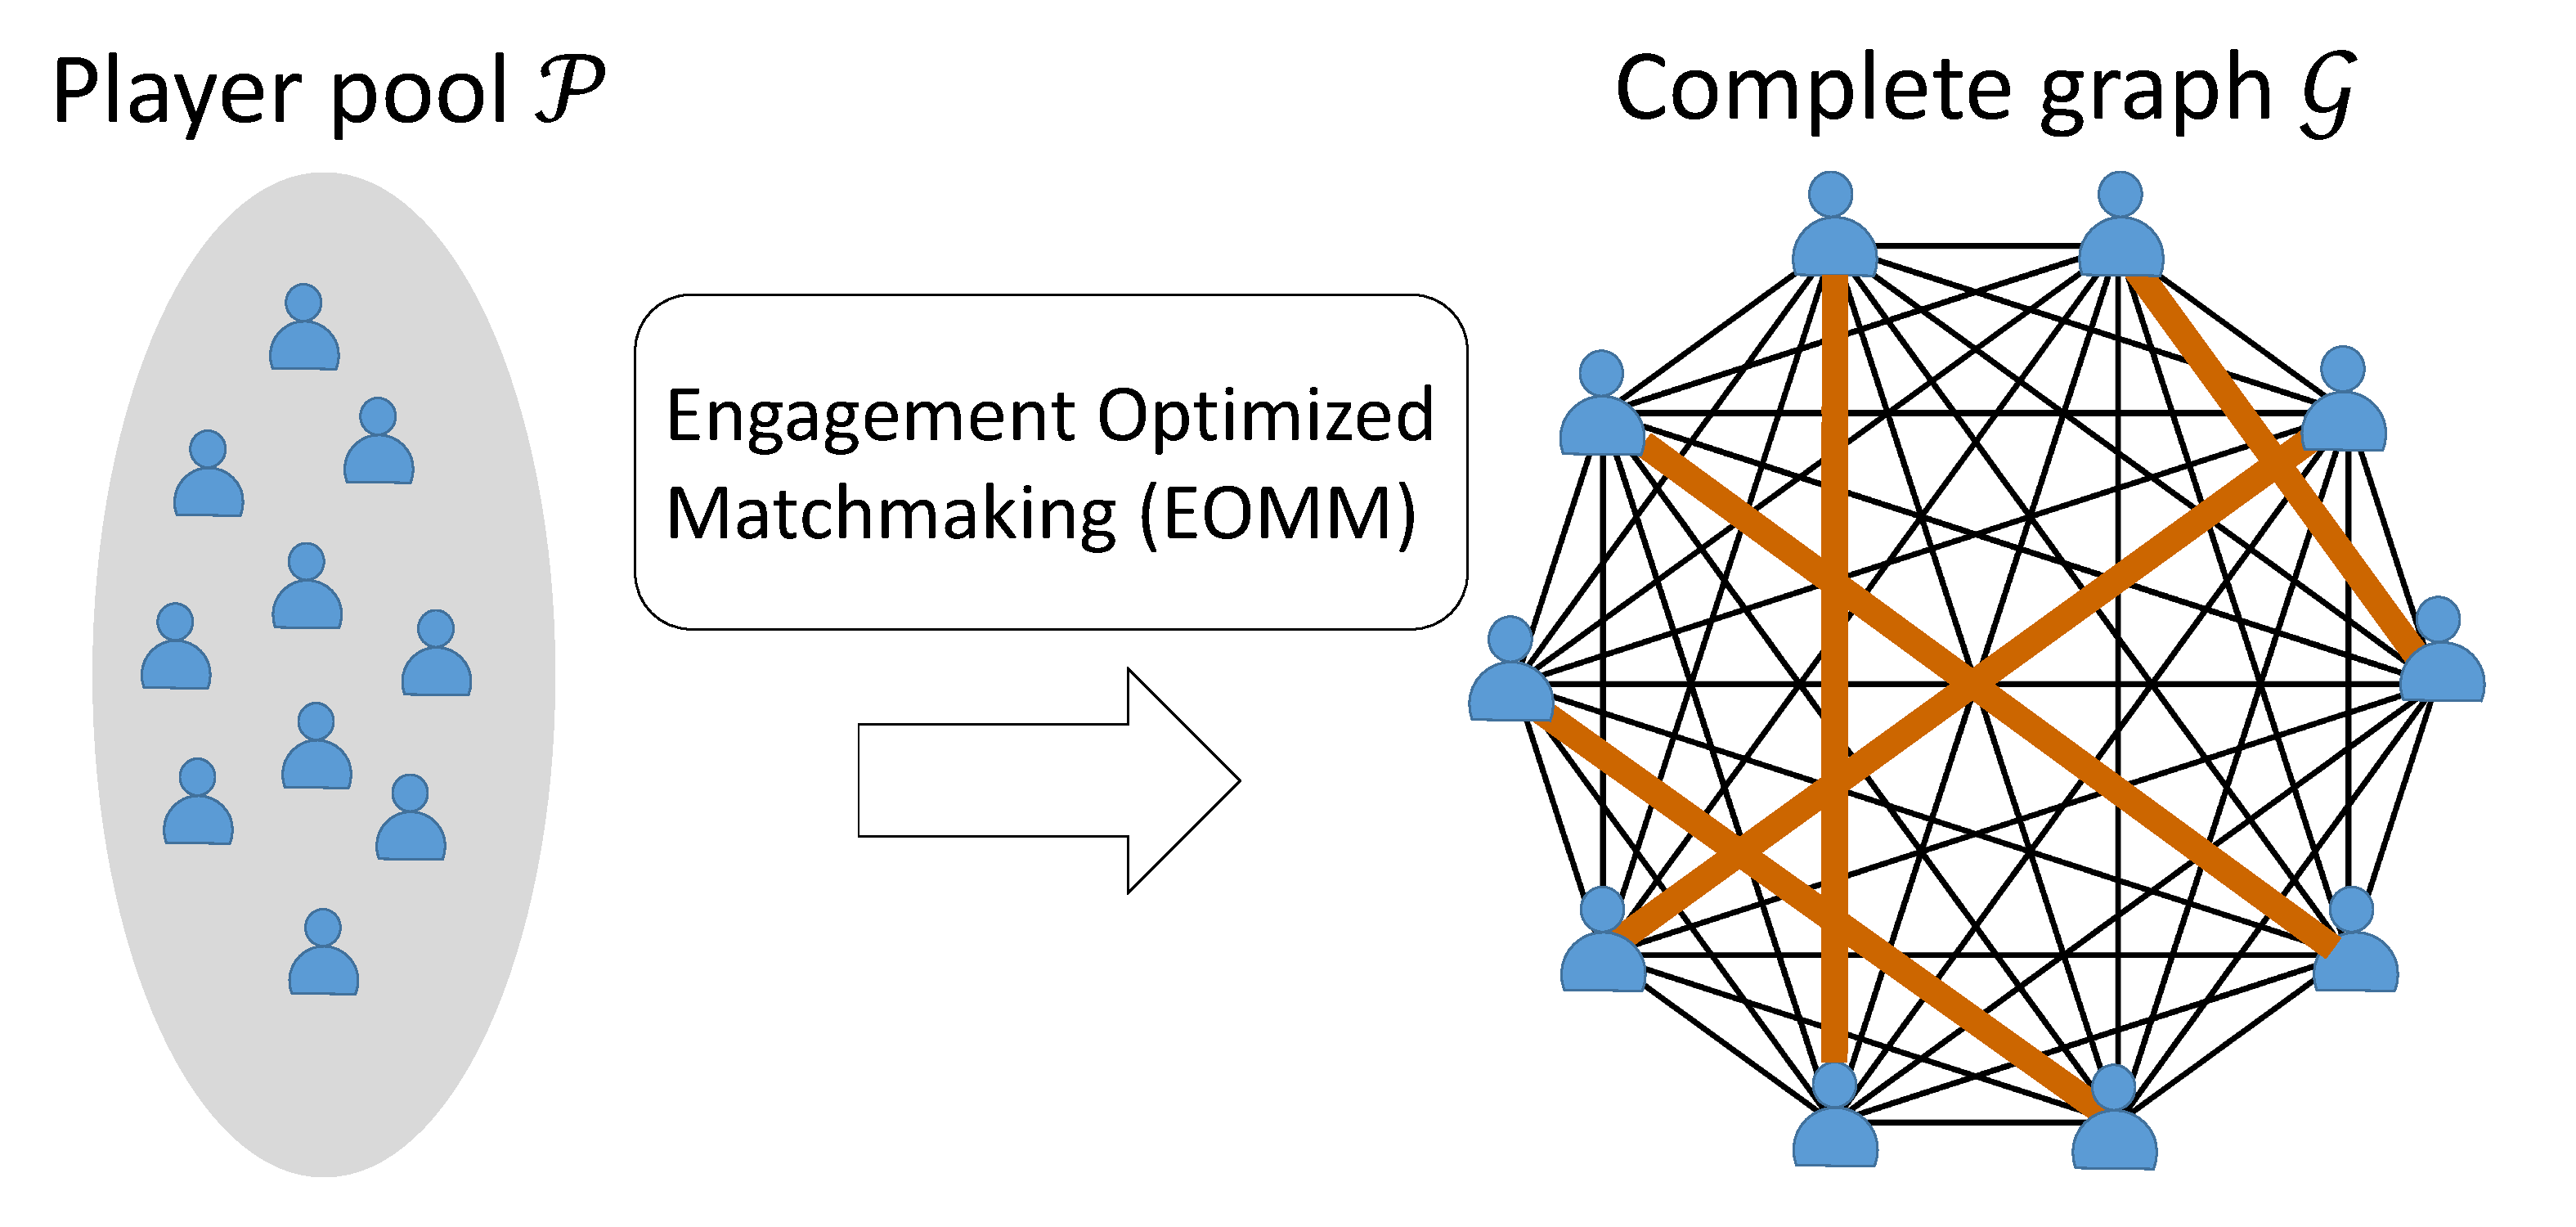
\includegraphics[width=1\textwidth]{Figures/complete_matching.pdf}
\caption{Model matchmaking on a complete graph. Each node represents a player, and every edge is associated with the sum engagement metric of two players if paired. EOMM amounts to finding an optimal pair assignment on $\mathcal{G}$.}
\label{fig:matching}
\end{figure}


\subsection{Predicting Churn Risks}\label{sec:churn}
We learn the function $c_{i,j} = c(\vect{s}_i, \vect{s}_j)$ as a churn prediction problem. In its original form, the churn risk $c_{i,j}$ of player $p_i$ after matchmaking depends on the states from both the player and their opponent. Unfortunately, the well-established churn prediction studies cannot be employed here, because they only use features of players themselves without considering those of opponents. Also, naively feeding both player states as input will double the feature dimension, which makes the prediction unintelligible and harder since much more training data is needed. 

One way to simplify the prediction of $c_{i,j}$ is to base it only on player $p_i$'s own state, $\vect{s}_i$, and the resulting match outcome, $o_{i,j}$, from the view of $p_i$. This works because the opponent's state, $\vect{s}_j$, such as skill, play history and style, does not directly interact with player $p_i$'s churn risk $c_{i,j}$. It, however, influences the upcoming match outcome, which is directly perceivable by player $p_i$ and thus affects $p_i$'s churn. Once the match outcome $o_{i,j}$ is known, $c_{i,j}$ becomes conditionally independent to the opponent's state, $\vect{s}_j$. Formally, this property is represented as:
\begin{equation}\label{eqn:dependency_raw}
\Pr(p_i \text{ churns} | \vect{s}_i, \vect{s}_j, o_{i,j}) = \Pr(p_i \text{ churns} | \vect{s}_i, o_{i,j}),
\end{equation}
which can be written in a concise form:
\begin{equation}\label{eqn:dependency}
c(\vect{s}_i, \vect{s}_j, o_{i,j}) = c(\vect{s}_i, o_{i,j})
\end{equation}

In this chapter, we assume that game outcomes are sampled from a finite set, $\mathcal{O}$, such as \emph{Win}, \emph{Lose} and \emph{Draw}. For example, $o_{i,j}=W$ means that $p_i$ wins over $p_j$, while $o_{j,i}=L$ represents the same outcome from the view of $p_j$. To predict game outcomes, we employ the standard skill models~\cite{elo1978rating,glickman1999parameter} that are widely adopted in the video game industry. These models use both players' skills, which are a proxy of their entire player states, as the input for the prediction. We denote player $p_i$'s skill representation as $\vect{\mu}_i$, which is, for example, Elo score~\cite{elo1978rating} or Glicko mean and RD~\cite{glickman1999parameter}. Note that $\vect{\mu}_i$ is part of player state $\vect{s}_i$.  As a result, we have:
\begin{equation}\label{eqn:skill}
\Pr(o_{i,j}|\vect{s}_i, \vect{s}_j) \approx \Pr(o_{i,j}|\vect{\mu}_i, \vect{\mu}_j),
\end{equation}

Putting them together, we can efficiently predict the churn risks of paired players in Eqn.~\ref{eqn:opt2}:
\begin{align}
&c(\vect{s}_i, \vect{s}_j) + c(\vect{s}_j, \vect{s}_i) \label{eqn:c1} \\
=& \sum\limits_{o_{i,j} \in \mathcal{O}} \Pr(o_{i,j}|\vect{s}_i, \vect{s}_j)\left( c(\vect{s}_i, \vect{s}_j, o_{i,j}) + c(\vect{s}_j, \vect{s}_i, o_{j,i}) \right) \label{eqn:c2} \\
\approx & \sum\limits_{o_{i,j} \in \mathcal{O}} \Pr(o_{i,j}|\vect{\mu}_i, \vect{\mu}_j)\left( c(\vect{s}_i, o_{i,j}) + c(\vect{s}_j, o_{j,i}) \right), \label{eqn:c3}
\end{align}
where the first equality is a marginalization on game outcome, $o_{i,j}$. In the approximate equality, the conditional independence of $c_{i,j}$ on $\vect{s}_j$ given $o_{i,j}$ (Eqn.~\ref{eqn:dependency}) and the game outcome prediction (Eqn.~\ref{eqn:skill}) are used.

Now $c(\vect{s}_i, o_{i,j})$ can be efficiently learned based on any preferred churn prediction model. The input features are the updated player state based on the predicted game outcome of the hypothetical matchmaking, i.e., $\vect{s}_i^{update} \leftarrow \vect{s}_i \text{ and } o_{i,j}$. We can decompose the original player state as $\vect{s}_i = [\vect{o}_i^K, \hat{\vect{s}}_i]$, where $\vect{o}_i^K$ is a vector of the latest $K$ game outcomes (for example, $\vect{o}_i^K=LWLDL$ when $K=5$), and $\hat{\vect{s}}_i$ represent the rest of features in $\vect{s}_i$. If $p_i$ is hypothetically matched with $p_j$, $\vect{s}_i$ will be updated as:
\begin{align}\label{eqn:stateUpdate}
\vect{s}_i^{update} \leftarrow& \vect{s}_i \text{ and } o_{i,j} \\
                    =& [\vect{o}_i^K, \hat{\vect{s}}_i] \text{ and } o_{i,j} \\
                    =& [\vect{o}_i^{K+1}, \hat{\vect{s}}_i^{update}]
\end{align}
We use $\hat{\vect{s}}_i^{update}$ to indicate that non-game-outcome features are also updated after the new match. For example, the total number of games played increments by one. 


%Then, we can adopt any preferred churn prediction model based on $\vect{s}_i^{update}$ in order to compute $c(\vect{s}_i, o_{i,j})$.
\vspace{2mm}

\subsection{Finding the Optimal Pair Assignment}
Given the predicted churn risks of each pair of players, i.e., the weight of every edge in $\mathcal{G}$, EOMM reduces to a minimum weight perfect matching (MWPM) problem. The goal is to find a pair assignment, $\mathcal{M}^*$, on a complete graph, $\mathcal{G}$, which has the minimal sum weights of edges.

For a graph with $N$ node, the brute-force method is to compare all $\binom N{N/2} / 2^{\frac{N}{2}}$ possible pair assignments and find the best one, but the time complexity is too high to be feasible in practical systems. Fortunately, many polynomial time algorithms exist for the MWPM problem. For example, several algorithms can solve the problem in the worst time complexity $O(N^3)$ \cite{gabow1974implementation,lawler2001combinatorial}. If engagement measurements are pure integers, there exists a slightly faster algorithm \cite{gabow1985scaling} with running time $O(N^{2\frac{3}{4}}\log K)$ where $K$ is the largest magnitude of an edge weight. There also exist greedy algorithms, such as \cite{drake2003simple} and \cite{duan2014linear}, with faster running time to find suboptimal solutions. Moreover, MWPM can be solved in parallel as proposed by \cite{osiakwan1990maximum}.

\vspace{3mm}

\section{Theoretical Findings}\label{sec:findings}
Besides generating optimal matchmaking assignments, EOMM provides a framework to conduct theoretical analysis on other matchmaking related problems. We use this framework to compare EOMM with other matchmaking strategies under different hypothetical situations to obtain many insights. Without loss of generality, we focus our discussion on 1-vs-1 games with possible game outcomes sampled from \emph{Win}, \emph{Lose} and \emph{Draw}.

Using the same notation in Section~\ref{sec:optimization}, we investigate a pair of players $p_i, p_j \in \mathcal{P}, i \neq j$. When $c(\vect{s}_i, \vect{s}_j) = c(o_{i,j})$, i.e., a player's churn risk only depends on the game outcome of the upcoming match, regardless of all other states. This simplification for Eqn.~\ref{eqn:stateUpdate}, where $\vect{s}_i^{update}$ only considers $o_{i,j}$ but ignores $\vect{s}_i$, has  interesting implications.
\begin{itemize}
\item If $c(Win)+c(Lose) > 2\cdot c(Draw)$, i.e., the sum churn risk of two matched players in a tied game is lower than that in a non-tied game. Under this circumstance, the equal-skill based matchmaking is \emph{equivalent} to EOMM, as both strive to form matches with \emph{Draw} outcomes as many as possible. This explains the intuition and popularity behind equal-skill matchmaking. But we should be aware of its conditional applicability, while EOMM is instead always optimal.
\item If $c(Win) + c(Lose)< 2\cdot c(Draw)$, equal-skill based matchmaking is actually \emph{worst} among all matchmaking schemes, as its goal to create close matches contrarily minimizes the overall player engagement. Although this situation contradicts with the common intuition that fair matches are good, it is possible for a real game. Therefore, validating the assumptions with real game data is critical before applying an equal-skill based matchmaking algorithm.
\end{itemize}

When $c(\vect{s}_i, \vect{s}_j) = c(\vect{s}_i)$, i.e., a player's churn risk is determined by his state before matchmaking, then it does not matter whom they will play. In this case, EOMM can do no better than a random matchmaking. Random matchmaking, from this perspective, is not trivial. It is a relative safe and stable baseline choice in lack of prior information. While equal-skill based method can perform the worst under certain conditions, random matchmaking will never fall into the worst case.

The analysis above shows that the existing matchmaking methods, such as equal-skill based and random matching, arise within the EOMM framework on different conditions. Practitioners can safely apply EOMM while gathering more information about their game and players.

\section{Case Study}\label{sec:casestudy}
To test the proposed matchmaking framework, we ran simulation which is configured based on the real data from a popular PvP game made by Electronic Arts Inc.\! (EA). In the simulation, we compared different matchmaking methods applied to the same player population. In the end, EOMM retained significantly higher number of players than other matchmaking methods.

\subsection{Data Collection}
We collected 1-vs-1 matches from a popular game made by EA. There are three possible match outcomes, namely \emph{Win}, \emph{Lose} and \emph{Draw}. In total, we collected 36.9 million matches played by 1.68 million unique players in the first half of 2016.

\subsection{Preparation}\label{sec:preprosessing}

\begin{figure}[t]
\centering
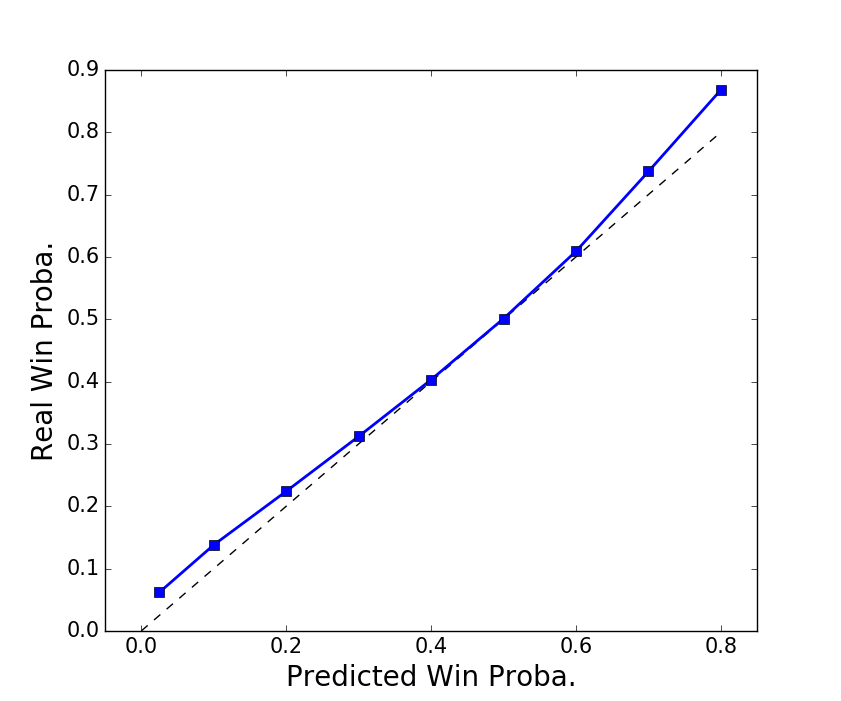
\includegraphics[width=0.8\textwidth]{Figures/prob_calib_glicko_line.png}
\caption{Predicted win probability vs. real win probability. Real win probability is the ratio of matches, with similar predicted winning probabilities, whose outcomes are real ``Wins''.  }
\label{fig:glicko_cali}
\end{figure}


To create a realistic environment for simulation, the following models and functions are needed. We compute them based on real game data.

\textbf{Player Skills} We need to establish a distribution of player skills for the population we simulate on. The distribution is learned from real game data. We sorted the collected real matches temporally and applied Glicko~\cite{glickman1999parameter} to compute each player's final skill. For each player $i$, the skill vector is represented by mean $r_i$ and variance $RD_i$, i.e. $\vect{\mu}_i = (r_i, RD_i)$. In simulation, we assume that the game and player skills are stationary. The population's skill distribution is constant, where each player's skill does not change any more over time.

% We chose to update Glicko ratings of involved players after every match. The estimated player skills were stored in a HashMap-like data structure indexed by player identities.

While Glicko scores can be used to estimate the winning probability of player $i$ over player $j$, $\Pr(i > j | \vect{\mu}_i, \vect{\mu}_j)$, they cannot provide the probability of draws. We defined a set of rules to allow the estimation of win/lose/draw probabilities from Glicko scores:
\begin{align}\label{eqn:draw}
\text{Pr}^*(i=j) = 20\%
\end{align}

\begin{align}
\text{Pr}^*(i>j)  = \frac{80\% \cdot \Pr(i > j | \vect{\mu}_i, \vect{\mu}_j)}{\Pr(i > j | \vect{\mu}_i, \vect{\mu}_j) + \Pr(j > i | \vect{\mu}_j, \vect{\mu}_i) }
\end{align}

\begin{align}
\text{Pr}^*(i<j) = 1 - \text{Pr}^*(i=j) - \text{Pr}^*(i>j)
\end{align}

% All the roofs of the bars are around the diagonal (dashed line), suggesting predicted win ratios by our rules are well calibrated.
Basically, the draw probability (Eqn.~\ref{eqn:draw}) is set to $20\%$ regardless of skill gaps. This is based on our findings that 1) draw outcomes only have $-0.05$ correlation with the difference of skill means in the collected game data; 2) around $20\%$ matches are draws regardless of skill gaps. The win/lose probabilities are normalized such that the probabilities of win, lose and draw sum up to 1. Figure~\ref{fig:glicko_cali} shows that the predicted win probabilities using Glicko scores based on our rules are well aligned with the real match outcomes.

\textbf{Churn Prediction Model} We trained a logistic regression model for predicting whether a player will be an eight-hour churner after a match. The input features describe the upcoming match and the player's 10 most recent matches. A player is labeled as an eight-hour churner if they do not play any 1-vs-1 match within the next eight hours after playing this match. As discussed in Section~\ref{sec:optimization}, the term of ``churn'' is used by convention. It represents ``stopping playing'' within a period of time, which is a metric of disengagement.

\begin{figure}[t]
\centering
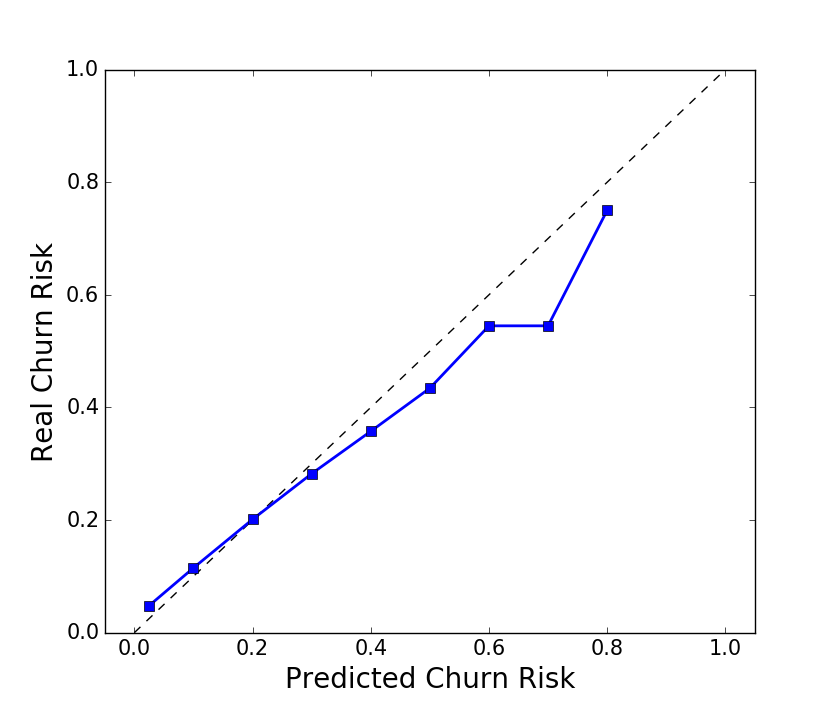
\includegraphics[width=0.8\textwidth]{Figures/prob_calib_lr_line.png}
\caption{Predicted churn risk vs. real churn risk. Real churn risk is the ratio of matches, with similar predicted churn risks, which are indeed the last match before churn. }
\label{fig:lr_cali}
\end{figure}

We use Eqn.~\ref{eqn:c3} to estimate $c(\vect{s}_i, \vect{s}_j) + c(\vect{s}_j, \vect{s}_i)$. The model takes as input the player's state $\vect{s}_i$ before matchmaking along with the upcoming match outcome $o_{i, j}$.

Specifically, the input features consist of:
\begin{itemize}
\item \textit{Each of the player's 10 most recent matches}: win/lose/draw status, time passage since the previous match, time passage to the upcoming match, and goal difference against his opponent
\item \textit{Upcoming match}: one-hot encoding of the upcoming match's outcome win/lose/draw
\item \textit{Other}: the number of 1-vs-1 matches played in the last eight hours, one day, one week and one month.
\end{itemize}

%The size of extracted data points after random sampling is 10 million. The ratio between positive (churned) and negative (not churned) labels is approximately 1:3.
% The range of grid search is from $10^{-3} \sim 10^3$.
% The performance of the best model (in terms of F1 score) is listed in Table 3 (averaged over 5 hold-out sample sets).

We use 5-fold cross validation and grid search to determine the proper $L_2$ regularization strength when training the model. The predicted probabilities are well aligned with the real churn probabilities, in particular when churn risk is less than 0.8, as shown in Figure~\ref{fig:lr_cali}. While the performance of the predictive model still has room to improve, the flexibility of EOMM allows one to easily refine or replace the model if better ones are found.

%One can easily notice that the recall of the best model is very low. This is due to the skewness of  labels of the dataset and the insufficient power of selected features to capture  churn patterns. To train a churn model performing more accurate classification, one can incorporate weights for data points \cite{lee2003learning} \footnote{if we adjust weights of data points inversely proportional to class frequencies in the input data, we can obtain a logistic regression model with 60.96\% accuracy, 66.66\% AUC, 63.65\% recall, 34.35\% precision and 0.4462 F1-score. (All metrics are averaged over 5 hold-out sample sets.)}, conduct more sophisticated feature engineering and test with more advanced models. However, the most important property of an engagement predictive model desired by EOMM should be that its predicting probabilities are well calibrated such that $G(\vect{s}_i, \vect{s}_j)$ is unbiased. We should think the logistic regression model as a churn risk estimator, rather than an accurate binary classifier. Since the logistic regression model directly optimizes for log-likelihood, its prediction probabilities are well aligned with real data, as shown in Figure~\ref{fig:lr_cali}. Therefore, we think the trained model is desirable in this case study primarily as an illustration of the applicability of EOMM.



%
%\begin{table}[]
%\centering
%\ra{1.1}
%\caption{Performance Evaluation on Churn Prediction Model}
%\begin{tabular}{ccccc}
%\hline
%Accuracy & AUC & Recall & Precision & F1-Score\\ \hline
%75.23\% & 64.21\% & 3.48\%  & 48.18\% & 0.0650 \\ \hline
%\end{tabular}
%\end{table}
% AUC is close to other papers?


\textbf{Player States} In simulation, each player's state is sampled from a collection of states, which are established based on real players' states in the collected data. We first randomly sample a subset of matches. Both players' states in those matches are gathered to create this collection. A player state contains the needed features for churn prediction, as well as the player's skill score.

% In total, the size of the player state sample pool is 10 million.
%We avoided player state samples or training data for the engagement prediction model that less than 15 recent matches are available for a player to be filled in. One should acknowledge that dealing with casual players is hard in practice and it is out of our scope.

%\newpage
\subsection{Simulation Procedure}
In the simulation, we compared EOMM with three matchmaking mechanisms: \textit{random matchmaking} (\textit{RandomMM}), which randomly pairs available players in the waiting pool, \textit{skill-based matchmaking} (\textit{SkillMM}), which pairs every two consecutive players after sorting them by skills, and \textit{worst matchmaking} (\textit{WorstMM}), which does the opposite of EOMM by minimizing the objective function of EOMM. SkillMM always seeks ``fair games''. We added WorstMM as a validation.

All methods are applied on the same population (waiting pool), where the same player skill distribution, churn model and player state distribution as described in Section~\ref{sec:preprosessing} are used. EOMM follows Eqn.~\ref{eqn:c3} to estimate churn risk $c(\vect{s}_i, \vect{s}_j) + c(\vect{s}_j, \vect{s}_i)$. We used the perfect matching algorithm \citep{gabow1974implementation,lawler2001combinatorial} implemented by an open-source library \citep{onlineperfectmatching}.



For each matchmaking method $\mathcal{M}$, the procedure within each round of simulation is as follows:
\begin{enumerate}
\item Create a waiting pool of $P$ players, whose player states are sampled from the player state collection.
\item Use $\mathcal{M}$ to determine the pair assignment (matchmaking).
\item Simulate match outcomes according to the win/lose/draw probability predicted by the skill model
\item For each player, simulate if he will churn according to the predicted churn probability by churn model.
\item Record the number of retained players.
\end{enumerate}

In experiments, we tested $P=100, 200, 300, 400$ and $500$. For each setting of $P$, we repeated the simulation by 10,000 rounds of matchmaking. We compare different matchmaking methods by the average number of their retained players per round, i.e., the players who continue playing in the next eight hours. In order to test statistical significance, we conducted Welch's $t$-test between every pair of the matchmaking algorithms.

%\begin{table*}[]
%\centering
%\ra{1.1}
%\caption{P-Values of Pairwise Welch's T-Tests}
%\begin{tabular}{lccccc}
%\hline
%\multicolumn{1}{c}{Method}                  & \multicolumn{5}{c}{p-value}    \\
%& \multicolumn{1}{c}{N=100} & \multicolumn{1}{c}{N=200} & \multicolumn{1}{c}{N=300} & \multicolumn{1}{c}{N=400} & \multicolumn{1}{c}{N=500} \\ \hline
%EOMM vs. WorstMM        & 1.83e-08**  & 2.24e-20**  & 6.25e-133**  & 3.45e-77**  & 2.36e-84** \\ \hline
%EOMM vs. SkillMM        & 1.43e-18**  & 2.84e-03**  & 1.95e-33**   & 3.55e-40**  & 2.50e-37** \\ \hline
%EOMM vs. RandomMM       & 2.16e-01  & 3.82e-03**  & 2.86e-33**   & 2.28e-53**  & 3.77e-23** \\ \hline
%SkillMM vs. WorstMM     & 6.73e-48**  & 5.62e-10**  & 1.19e-33**   & 2.55e-08**  & 1.08e-11** \\ \hline
%SkillMM vs. RandomMM    & 8.89e-24**  & 9.23e-01**  & 7.52e-01   & 1.71e-02*  & 5.98e-03** \\ \hline
%RandomMM vs. WorstMM    & 1.14e-05**  & 2.77e-10**  & 6.51e-37**   & 1.88e-03**  & 3.03e-21** \\ \hline
%\end{tabular}
%\end{table*}






\subsection{Results and Discussion}

The results are shown in Table~\ref{tab:result}. All pairwise differences of retained players are statistically significant ($p$-value $< 0.01$) except EOMM vs.\! RandomMM (when $P=100$) and SkillMM vs.\! RandomMM (when $P=400$). In all other scenarios, EOMM outperforms the other three matchmaking methods. The results prove the applicability of EOMM to act as an engagement optimizer. When $P=100$, EOMM does not retain a significantly higher number of players than RandomMM, and even retains fewer players than SkillMM. It is possibly because that when $P$ is small, the randomness has higher impact, and also, the room for arranging opponents is smaller. More rounds of simulations might be needed to show significance in this case.

The improvement of EOMM over SkillMM, the most common matchmaking method, in terms of the average number of retained players are $0.3\%$, $0.9\%$, $1.1\%$, and $0.6\%$ when $P=200, 300, 400$ and $500$ respectively. On average EOMM retains $0.7\%$ more player compared with SkillMM after one round of matchmaking. Notably the benefit of retention will accumulate over time in a constant population. For players who play 20 rounds of matchmaking games within eight hours, there will be $15\%$ more players retained ($1.007^{20}$ $ \approx 1.15$) by EOMM over those by SkillMM. The more rounds of matchmaking are conducted, the more significant is the accumulative advantage of EOMM in engagement.

We did not find a consistent climb in retention boost as $P$ increased. This may suggest that when the player pool reaches certain size, the choices of opponents are enough to rescue those players on the edge of churn. Beyond this size, a larger player pool may not bring in significantly extra benefits in engagement maximization.

As a validation, WorstMM consistently retains the fewest players in the pools of all sizes. This result verifies the optimum of EOMM from the opposite side. It is also interesting to note that SkillMM does not consistently outperform RandomMM, which is aligned with our discussion in the theoretical findings in Section~\ref{sec:findings}, that is, balanced matches are not always optimal for engagement.


\begin{table}[t]
\centering
\ra{1.1}
\caption{Average number of retained players per round of matchmaking simulation. 10,000 rounds of matchmaking were simulated.}
\label{tab:result}
\begin{tabular}{lccccc}
\hline
\emph{Method} & \multicolumn{1}{c}{P=100} & \multicolumn{1}{c}{P=200} & \multicolumn{1}{c}{P=300} & \multicolumn{1}{c}{P=400} & \multicolumn{1}{c}{P=500} \\ \hline
WorstMM  & 51.50   & 103.39   & 154.57    & 206.65  &  258.21  \\ \hline
SkillMM  & 52.52   & 103.96   & 156.05    & 207.43  &  259.24  \\ \hline
RandomMM & 51.81   & 103.97   & 156.09    & 207.09  &  259.65  \\ \hline
EOMM     & 51.90   & 104.24   & 157.50    & 209.37  &  261.19  \\ \hline
\end{tabular}
\end{table}



\section{Summary}
This chapter attempts to answer \hyperref[rq2]{\textbf{R.S.Q.~2}} by presenting a novel framework, Engagement Optimized Matchmaking (EOMM), to achieve optimized engagement for a population of online players through recommendation of opponents. It formulates matchmaking as a problem of maximizing the player engagement, and solves the optimization efficiently. EOMM employs three components, a skill model, an engagement predictive model and a minimum weight perfect matching algorithm, each of which can be tailored flexibly for specific applications. We ran simulations whose configurations were based on real data from an online PvP game. The results show that EOMM significantly outperforms all other methods in the number of retained players. EOMM also provides a theoretical framework to analyze various matchmaking algorithms.

EOMM provides a measurable and flexible matchmaking framework. It has well-defined quantitative objectives that can be monitored, evaluated and improved. Within the EOMM framework, the core building components, skill model, churn model and graph pairing model, are uncoupled so that they can be tuned and replaced independently. Moreover, we can even change the objective function to other data-driven metrics of player engagement, such as play time, retention, or spending. EOMM allows one to easily plug in different types of predictive models to achieve the optimization.

% So far we have discussed EOMM in 1-vs-1 game scenarios. This framework also applies to PvP games that involve teams of players, where every component needs to be extended with additional care. The skill model can be simply applied to a team by adding up skills for all team members~\cite{herbrich:trueskill}. For churn prediction, we can use the same idea that one player's churn risk is conditionally independent with other players' states given that their influence on the player's own state, such as the game outcome, is known. Last, the minimum weight perfect matching algorithms for pairs are no longer applicable. Instead of a pair assignment, we seek a \emph{grouping assignment} on a complete graph. A related area to investigate is perfect matching in hypergraphs~\cite{berge1984hypergraphs}, where an edge can connect more than two vertices. Furthermore, EOMM is not even limited to games. In broad applications, such as friend connection in a social network and 1-on-1 tutoring in online education, EOMM's formulation and optimization techniques still apply.

% In the future, we expect EOMM equipped with more advanced models, such as skill model and churn model, can have higher optimal bound. We will explore EOMM performance in more realistic situations, where practical restrictions are applied, such as network connectivity, regions and friend/black lists. More restrictions would result in fewer edges in the constructed graph of EOMM. Last, we will explore EOMM in multi-player games with more than two players involved and efficient algorithms analogous to perfect matching algorithms within hypergraphs. 
\chapter{Conclusion and Future Work} % Main chapter title

\label{chapter:conclusion} 

Like most of existing recommendation systems, each of the recommendation systems proposed in my thesis deals with only a specific type of in-game content. The ultimate, and more ambitious, goal, is to design a unified recommendation system which could make central decisions on recommendations of various in-game content for a particular player. 
% % Chapter 1

\chapter{Chapter Title Here} % Main chapter title

\label{Chapter1} % For referencing the chapter elsewhere, use \ref{Chapter1} 

%----------------------------------------------------------------------------------------

% Define some commands to keep the formatting separated from the content 
\newcommand{\keyword}[1]{\textbf{#1}}
\newcommand{\tabhead}[1]{\textbf{#1}}
\newcommand{\code}[1]{\texttt{#1}}
\newcommand{\file}[1]{\texttt{\bfseries#1}}
\newcommand{\option}[1]{\texttt{\itshape#1}}

%----------------------------------------------------------------------------------------

\section{Welcome and Thank You}
Welcome to this \LaTeX{} Thesis Template, a beautiful and easy to use template for writing a thesis using the \LaTeX{} typesetting system.

If you are writing a thesis (or will be in the future) and its subject is technical or mathematical (though it doesn't have to be), then creating it in \LaTeX{} is highly recommended as a way to make sure you can just get down to the essential writing without having to worry over formatting or wasting time arguing with your word processor.

\LaTeX{} is easily able to professionally typeset documents that run to hundreds or thousands of pages long. With simple mark-up commands, it automatically sets out the table of contents, margins, page headers and footers and keeps the formatting consistent and beautiful. One of its main strengths is the way it can easily typeset mathematics, even \emph{heavy} mathematics. Even if those equations are the most horribly twisted and most difficult mathematical problems that can only be solved on a super-computer, you can at least count on \LaTeX{} to make them look stunning.

%----------------------------------------------------------------------------------------

\section{Learning \LaTeX{}}

\LaTeX{} is not a \textsc{wysiwyg} (What You See is What You Get) program, unlike word processors such as Microsoft Word or Apple's Pages. Instead, a document written for \LaTeX{} is actually a simple, plain text file that contains \emph{no formatting}. You tell \LaTeX{} how you want the formatting in the finished document by writing in simple commands amongst the text, for example, if I want to use \emph{italic text for emphasis}, I write the \verb|\emph{text}| command and put the text I want in italics in between the curly braces. This means that \LaTeX{} is a \enquote{mark-up} language, very much like HTML.

\subsection{A (not so short) Introduction to \LaTeX{}}

If you are new to \LaTeX{}, there is a very good eBook -- freely available online as a PDF file -- called, \enquote{The Not So Short Introduction to \LaTeX{}}. The book's title is typically shortened to just \emph{lshort}. You can download the latest version (as it is occasionally updated) from here:
\url{http://www.ctan.org/tex-archive/info/lshort/english/lshort.pdf}

It is also available in several other languages. Find yours from the list on this page: \url{http://www.ctan.org/tex-archive/info/lshort/}

It is recommended to take a little time out to learn how to use \LaTeX{} by creating several, small `test' documents, or having a close look at several templates on:\\ 
\url{http://www.LaTeXTemplates.com}\\ 
Making the effort now means you're not stuck learning the system when what you \emph{really} need to be doing is writing your thesis.

\subsection{A Short Math Guide for \LaTeX{}}

If you are writing a technical or mathematical thesis, then you may want to read the document by the AMS (American Mathematical Society) called, \enquote{A Short Math Guide for \LaTeX{}}. It can be found online here:
\url{http://www.ams.org/tex/amslatex.html}
under the \enquote{Additional Documentation} section towards the bottom of the page.

\subsection{Common \LaTeX{} Math Symbols}
There are a multitude of mathematical symbols available for \LaTeX{} and it would take a great effort to learn the commands for them all. The most common ones you are likely to use are shown on this page:
\url{http://www.sunilpatel.co.uk/latex-type/latex-math-symbols/}

You can use this page as a reference or crib sheet, the symbols are rendered as large, high quality images so you can quickly find the \LaTeX{} command for the symbol you need.

\subsection{\LaTeX{} on a Mac}
 
The \LaTeX{} distribution is available for many systems including Windows, Linux and Mac OS X. The package for OS X is called MacTeX and it contains all the applications you need -- bundled together and pre-customized -- for a fully working \LaTeX{} environment and work flow.
 
MacTeX includes a custom dedicated \LaTeX{} editor called TeXShop for writing your `\file{.tex}' files and BibDesk: a program to manage your references and create your bibliography section just as easily as managing songs and creating playlists in iTunes.

%----------------------------------------------------------------------------------------

\section{Getting Started with this Template}

If you are familiar with \LaTeX{}, then you should explore the directory structure of the template and then proceed to place your own information into the \emph{THESIS INFORMATION} block of the \file{main.tex} file. You can then modify the rest of this file to your unique specifications based on your degree/university. Section \ref{FillingFile} on page \pageref{FillingFile} will help you do this. Make sure you also read section \ref{ThesisConventions} about thesis conventions to get the most out of this template.

If you are new to \LaTeX{} it is recommended that you carry on reading through the rest of the information in this document.

Before you begin using this template you should ensure that its style complies with the thesis style guidelines imposed by your institution. In most cases this template style and layout will be suitable. If it is not, it may only require a small change to bring the template in line with your institution's recommendations. These modifications will need to be done on the \file{MastersDoctoralThesis.cls} file.

\subsection{About this Template}

This \LaTeX{} Thesis Template is originally based and created around a \LaTeX{} style file created by Steve R.\ Gunn from the University of Southampton (UK), department of Electronics and Computer Science. You can find his original thesis style file at his site, here:
\url{http://www.ecs.soton.ac.uk/~srg/softwaretools/document/templates/}

Steve's \file{ecsthesis.cls} was then taken by Sunil Patel who modified it by creating a skeleton framework and folder structure to place the thesis files in. The resulting template can be found on Sunil's site here:
\url{http://www.sunilpatel.co.uk/thesis-template}

Sunil's template was made available through \url{http://www.LaTeXTemplates.com} where it was modified many times based on user requests and questions. Version 2.0 and onwards of this template represents a major modification to Sunil's template and is, in fact, hardly recognisable. The work to make version 2.0 possible was carried out by \href{mailto:vel@latextemplates.com}{Vel} and Johannes Böttcher.

%----------------------------------------------------------------------------------------

\section{What this Template Includes}

\subsection{Folders}

This template comes as a single zip file that expands out to several files and folders. The folder names are mostly self-explanatory:

\keyword{Appendices} -- this is the folder where you put the appendices. Each appendix should go into its own separate \file{.tex} file. An example and template are included in the directory.

\keyword{Chapters} -- this is the folder where you put the thesis chapters. A thesis usually has about six chapters, though there is no hard rule on this. Each chapter should go in its own separate \file{.tex} file and they can be split as:
\begin{itemize}
\item Chapter 1: Introduction to the thesis topic
\item Chapter 2: Background information and theory
\item Chapter 3: (Laboratory) experimental setup
\item Chapter 4: Details of experiment 1
\item Chapter 5: Details of experiment 2
\item Chapter 6: Discussion of the experimental results
\item Chapter 7: Conclusion and future directions
\end{itemize}
This chapter layout is specialised for the experimental sciences, your discipline may be different.

\keyword{Figures} -- this folder contains all figures for the thesis. These are the final images that will go into the thesis document.

\subsection{Files}

Included are also several files, most of them are plain text and you can see their contents in a text editor. After initial compilation, you will see that more auxiliary files are created by \LaTeX{} or BibTeX and which you don't need to delete or worry about:

\keyword{example.bib} -- this is an important file that contains all the bibliographic information and references that you will be citing in the thesis for use with BibTeX. You can write it manually, but there are reference manager programs available that will create and manage it for you. Bibliographies in \LaTeX{} are a large subject and you may need to read about BibTeX before starting with this. Many modern reference managers will allow you to export your references in BibTeX format which greatly eases the amount of work you have to do.

\keyword{MastersDoctoralThesis.cls} -- this is an important file. It is the class file that tells \LaTeX{} how to format the thesis. 

\keyword{main.pdf} -- this is your beautifully typeset thesis (in the PDF file format) created by \LaTeX{}. It is supplied in the PDF with the template and after you compile the template you should get an identical version.

\keyword{main.tex} -- this is an important file. This is the file that you tell \LaTeX{} to compile to produce your thesis as a PDF file. It contains the framework and constructs that tell \LaTeX{} how to layout the thesis. It is heavily commented so you can read exactly what each line of code does and why it is there. After you put your own information into the \emph{THESIS INFORMATION} block -- you have now started your thesis!

Files that are \emph{not} included, but are created by \LaTeX{} as auxiliary files include:

\keyword{main.aux} -- this is an auxiliary file generated by \LaTeX{}, if it is deleted \LaTeX{} simply regenerates it when you run the main \file{.tex} file.

\keyword{main.bbl} -- this is an auxiliary file generated by BibTeX, if it is deleted, BibTeX simply regenerates it when you run the \file{main.aux} file. Whereas the \file{.bib} file contains all the references you have, this \file{.bbl} file contains the references you have actually cited in the thesis and is used to build the bibliography section of the thesis.

\keyword{main.blg} -- this is an auxiliary file generated by BibTeX, if it is deleted BibTeX simply regenerates it when you run the main \file{.aux} file.

\keyword{main.lof} -- this is an auxiliary file generated by \LaTeX{}, if it is deleted \LaTeX{} simply regenerates it when you run the main \file{.tex} file. It tells \LaTeX{} how to build the \emph{List of Figures} section.

\keyword{main.log} -- this is an auxiliary file generated by \LaTeX{}, if it is deleted \LaTeX{} simply regenerates it when you run the main \file{.tex} file. It contains messages from \LaTeX{}, if you receive errors and warnings from \LaTeX{}, they will be in this \file{.log} file.

\keyword{main.lot} -- this is an auxiliary file generated by \LaTeX{}, if it is deleted \LaTeX{} simply regenerates it when you run the main \file{.tex} file. It tells \LaTeX{} how to build the \emph{List of Tables} section.

\keyword{main.out} -- this is an auxiliary file generated by \LaTeX{}, if it is deleted \LaTeX{} simply regenerates it when you run the main \file{.tex} file.

So from this long list, only the files with the \file{.bib}, \file{.cls} and \file{.tex} extensions are the most important ones. The other auxiliary files can be ignored or deleted as \LaTeX{} and BibTeX will regenerate them.

%----------------------------------------------------------------------------------------

\section{Filling in Your Information in the \file{main.tex} File}\label{FillingFile}

You will need to personalise the thesis template and make it your own by filling in your own information. This is done by editing the \file{main.tex} file in a text editor or your favourite LaTeX environment.

Open the file and scroll down to the third large block titled \emph{THESIS INFORMATION} where you can see the entries for \emph{University Name}, \emph{Department Name}, etc \ldots

% Fill out the information about yourself, your group and institution. You can also insert web links, if you do, make sure you use the full URL, including the \code{http://} for this. If you don't want these to be linked, simply remove the \verb|\href{url}{name}| and only leave the name.

When you have done this, save the file and recompile \code{main.tex}. All the information you filled in should now be in the PDF, complete with web links. You can now begin your thesis proper!

%----------------------------------------------------------------------------------------

\section{The \code{main.tex} File Explained}

The \file{main.tex} file contains the structure of the thesis. There are plenty of written comments that explain what pages, sections and formatting the \LaTeX{} code is creating. Each major document element is divided into commented blocks with titles in all capitals to make it obvious what the following bit of code is doing. Initially there seems to be a lot of \LaTeX{} code, but this is all formatting, and it has all been taken care of so you don't have to do it.

Begin by checking that your information on the title page is correct. For the thesis declaration, your institution may insist on something different than the text given. If this is the case, just replace what you see with what is required in the \emph{DECLARATION PAGE} block.

Then comes a page which contains a funny quote. You can put your own, or quote your favourite scientist, author, person, and so on. Make sure to put the name of the person who you took the quote from.

Following this is the abstract page which summarises your work in a condensed way and can almost be used as a standalone document to describe what you have done. The text you write will cause the heading to move up so don't worry about running out of space.

Next come the acknowledgements. On this page, write about all the people who you wish to thank (not forgetting parents, partners and your advisor/supervisor).

The contents pages, list of figures and tables are all taken care of for you and do not need to be manually created or edited. The next set of pages are more likely to be optional and can be deleted since they are for a more technical thesis: insert a list of abbreviations you have used in the thesis, then a list of the physical constants and numbers you refer to and finally, a list of mathematical symbols used in any formulae. Making the effort to fill these tables means the reader has a one-stop place to refer to instead of searching the internet and references to try and find out what you meant by certain abbreviations or symbols.

The list of symbols is split into the Roman and Greek alphabets. Whereas the abbreviations and symbols ought to be listed in alphabetical order (and this is \emph{not} done automatically for you) the list of physical constants should be grouped into similar themes.

The next page contains a one line dedication. Who will you dedicate your thesis to?

Finally, there is the block where the chapters are included. Uncomment the lines (delete the \code{\%} character) as you write the chapters. Each chapter should be written in its own file and put into the \emph{Chapters} folder and named \file{Chapter1}, \file{Chapter2}, etc\ldots Similarly for the appendices, uncomment the lines as you need them. Each appendix should go into its own file and placed in the \emph{Appendices} folder.

After the preamble, chapters and appendices finally comes the bibliography. The bibliography style (called \option{authoryear}) is used for the bibliography and is a fully featured style that will even include links to where the referenced paper can be found online. Do not underestimate how grateful your reader will be to find that a reference to a paper is just a click away. Of course, this relies on you putting the URL information into the BibTeX file in the first place.

%----------------------------------------------------------------------------------------

\section{Thesis Features and Conventions}\label{ThesisConventions}

To get the best out of this template, there are a few conventions that you may want to follow.

One of the most important (and most difficult) things to keep track of in such a long document as a thesis is consistency. Using certain conventions and ways of doing things (such as using a Todo list) makes the job easier. Of course, all of these are optional and you can adopt your own method.

\subsection{Printing Format}

This thesis template is designed for double sided printing (i.e. content on the front and back of pages) as most theses are printed and bound this way. Switching to one sided printing is as simple as uncommenting the \option{oneside} option of the \code{documentclass} command at the top of the \file{main.tex} file. You may then wish to adjust the margins to suit specifications from your institution.

The headers for the pages contain the page number on the outer side (so it is easy to flick through to the page you want) and the chapter name on the inner side.

The text is set to 11 point by default with single line spacing, again, you can tune the text size and spacing should you want or need to using the options at the very start of \file{main.tex}. The spacing can be changed similarly by replacing the \option{singlespacing} with \option{onehalfspacing} or \option{doublespacing}.

\subsection{Using US Letter Paper}

The paper size used in the template is A4, which is the standard size in Europe. If you are using this thesis template elsewhere and particularly in the United States, then you may have to change the A4 paper size to the US Letter size. This can be done in the margins settings section in \file{main.tex}.

Due to the differences in the paper size, the resulting margins may be different to what you like or require (as it is common for institutions to dictate certain margin sizes). If this is the case, then the margin sizes can be tweaked by modifying the values in the same block as where you set the paper size. Now your document should be set up for US Letter paper size with suitable margins.

\subsection{References}

The \code{biblatex} package is used to format the bibliography and inserts references such as this one \parencite{Reference1}. The options used in the \file{main.tex} file mean that the in-text citations of references are formatted with the author(s) listed with the date of the publication. Multiple references are separated by semicolons (e.g. \parencite{Reference2, Reference1}) and references with more than three authors only show the first author with \emph{et al.} indicating there are more authors (e.g. \parencite{Reference3}). This is done automatically for you. To see how you use references, have a look at the \file{Chapter1.tex} source file. Many reference managers allow you to simply drag the reference into the document as you type.

Scientific references should come \emph{before} the punctuation mark if there is one (such as a comma or period). The same goes for footnotes\footnote{Such as this footnote, here down at the bottom of the page.}. You can change this but the most important thing is to keep the convention consistent throughout the thesis. Footnotes themselves should be full, descriptive sentences (beginning with a capital letter and ending with a full stop). The APA6 states: \enquote{Footnote numbers should be superscripted, [...], following any punctuation mark except a dash.} The Chicago manual of style states: \enquote{A note number should be placed at the end of a sentence or clause. The number follows any punctuation mark except the dash, which it precedes. It follows a closing parenthesis.}

The bibliography is typeset with references listed in alphabetical order by the first author's last name. This is similar to the APA referencing style. To see how \LaTeX{} typesets the bibliography, have a look at the very end of this document (or just click on the reference number links in in-text citations).

\subsubsection{A Note on bibtex}

The bibtex backend used in the template by default does not correctly handle unicode character encoding (i.e. "international" characters). You may see a warning about this in the compilation log and, if your references contain unicode characters, they may not show up correctly or at all. The solution to this is to use the biber backend instead of the outdated bibtex backend. This is done by finding this in \file{main.tex}: \option{backend=bibtex} and changing it to \option{backend=biber}. You will then need to delete all auxiliary BibTeX files and navigate to the template directory in your terminal (command prompt). Once there, simply type \code{biber main} and biber will compile your bibliography. You can then compile \file{main.tex} as normal and your bibliography will be updated. An alternative is to set up your LaTeX editor to compile with biber instead of bibtex, see \href{http://tex.stackexchange.com/questions/154751/biblatex-with-biber-configuring-my-editor-to-avoid-undefined-citations/}{here} for how to do this for various editors.

\subsection{Tables}

Tables are an important way of displaying your results, below is an example table which was generated with this code:

{\small
\begin{verbatim}
\begin{table}
\caption{The effects of treatments X and Y on the four groups studied.}
\label{tab:treatments}
\centering
\begin{tabular}{l l l}
\toprule
\tabhead{Groups} & \tabhead{Treatment X} & \tabhead{Treatment Y} \\
\midrule
1 & 0.2 & 0.8\\
2 & 0.17 & 0.7\\
3 & 0.24 & 0.75\\
4 & 0.68 & 0.3\\
\bottomrule\\
\end{tabular}
\end{table}
\end{verbatim}
}

\begin{table}
\caption{The effects of treatments X and Y on the four groups studied.}
\label{tab:treatments}
\centering
\begin{tabular}{l l l}
\toprule
\tabhead{Groups} & \tabhead{Treatment X} & \tabhead{Treatment Y} \\
\midrule
1 & 0.2 & 0.8\\
2 & 0.17 & 0.7\\
3 & 0.24 & 0.75\\
4 & 0.68 & 0.3\\
\bottomrule\\
\end{tabular}
\end{table}

You can reference tables with \verb|\ref{<label>}| where the label is defined within the table environment. See \file{Chapter1.tex} for an example of the label and citation (e.g. Table~\ref{tab:treatments}).

\subsection{Figures}

There will hopefully be many figures in your thesis (that should be placed in the \emph{Figures} folder). The way to insert figures into your thesis is to use a code template like this:
\begin{verbatim}
\begin{figure}
\centering

\includegraphics{Figures/Electron}
\decoRule
\caption[An Electron]{An electron (artist's impression).}
\label{fig:Electron}
\end{figure}
\end{verbatim}
Also look in the source file. Putting this code into the source file produces the picture of the electron that you can see in the figure below.

\begin{figure}[th]
\centering

\includegraphics{Figures/Electron}
\decoRule
\caption[An Electron]{An electron (artist's impression).}
\label{fig:Electron}
\end{figure}

Sometimes figures don't always appear where you write them in the source. The placement depends on how much space there is on the page for the figure. Sometimes there is not enough room to fit a figure directly where it should go (in relation to the text) and so \LaTeX{} puts it at the top of the next page. Positioning figures is the job of \LaTeX{} and so you should only worry about making them look good!

Figures usually should have captions just in case you need to refer to them (such as in Figure~\ref{fig:Electron}). The \verb|\caption| command contains two parts, the first part, inside the square brackets is the title that will appear in the \emph{List of Figures}, and so should be short. The second part in the curly brackets should contain the longer and more descriptive caption text.

The \verb|\decoRule| command is optional and simply puts an aesthetic horizontal line below the image. If you do this for one image, do it for all of them.

\LaTeX{} is capable of using images in pdf, jpg and png format.

\subsection{Typesetting mathematics}

If your thesis is going to contain heavy mathematical content, be sure that \LaTeX{} will make it look beautiful, even though it won't be able to solve the equations for you.

The \enquote{Not So Short Introduction to \LaTeX} (available on \href{http://www.ctan.org/tex-archive/info/lshort/english/lshort.pdf}{CTAN}) should tell you everything you need to know for most cases of typesetting mathematics. If you need more information, a much more thorough mathematical guide is available from the AMS called, \enquote{A Short Math Guide to \LaTeX} and can be downloaded from:
\url{ftp://ftp.ams.org/pub/tex/doc/amsmath/short-math-guide.pdf}

There are many different \LaTeX{} symbols to remember, luckily you can find the most common symbols in \href{http://ctan.org/pkg/comprehensive}{The Comprehensive \LaTeX~Symbol List}.

You can write an equation, which is automatically given an equation number by \LaTeX{} like this:
\begin{verbatim}
\begin{equation}
E = mc^{2}
\label{eqn:Einstein}
\end{equation}
\end{verbatim}

This will produce Einstein's famous energy-matter equivalence equation:
\begin{equation}
E = mc^{2}
\label{eqn:Einstein}
\end{equation}

All equations you write (which are not in the middle of paragraph text) are automatically given equation numbers by \LaTeX{}. If you don't want a particular equation numbered, use the unnumbered form:
\begin{verbatim}
\[ a^{2}=4 \]
\end{verbatim}

%----------------------------------------------------------------------------------------

\section{Sectioning and Subsectioning}

You should break your thesis up into nice, bite-sized sections and subsections. \LaTeX{} automatically builds a table of Contents by looking at all the \verb|\chapter{}|, \verb|\section{}|  and \verb|\subsection{}| commands you write in the source.

The Table of Contents should only list the sections to three (3) levels. A \verb|chapter{}| is level zero (0). A \verb|\section{}| is level one (1) and so a \verb|\subsection{}| is level two (2). In your thesis it is likely that you will even use a \verb|subsubsection{}|, which is level three (3). The depth to which the Table of Contents is formatted is set within \file{MastersDoctoralThesis.cls}. If you need this changed, you can do it in \file{main.tex}.

%----------------------------------------------------------------------------------------

\section{In Closing}

You have reached the end of this mini-guide. You can now rename or overwrite this pdf file and begin writing your own \file{Chapter1.tex} and the rest of your thesis. The easy work of setting up the structure and framework has been taken care of for you. It's now your job to fill it out!

Good luck and have lots of fun!

\begin{flushright}
Guide written by ---\\
Sunil Patel: \href{http://www.sunilpatel.co.uk}{www.sunilpatel.co.uk}\\
Vel: \href{http://www.LaTeXTemplates.com}{LaTeXTemplates.com}
\end{flushright}
 


%----------------------------------------------------------------------------------------
%	THESIS CONTENT - APPENDICES
%----------------------------------------------------------------------------------------

\appendix % Cue to tell LaTeX that the following "chapters" are Appendices

% Include the appendices of the thesis as separate files from the Appendices folder
% Uncomment the lines as you write the Appendices

% % Appendix A

\chapter{Frequently Asked Questions} % Main appendix title

\label{AppendixA} % For referencing this appendix elsewhere, use \ref{AppendixA}

\section{How do I change the colors of links?}

The color of links can be changed to your liking using:

{\small\verb!\hypersetup{urlcolor=red}!}, or

{\small\verb!\hypersetup{citecolor=green}!}, or

{\small\verb!\hypersetup{allcolor=blue}!}.

\noindent If you want to completely hide the links, you can use:

{\small\verb!\hypersetup{allcolors=.}!}, or even better: 

{\small\verb!\hypersetup{hidelinks}!}.

\noindent If you want to have obvious links in the PDF but not the printed text, use:

{\small\verb!\hypersetup{colorlinks=false}!}.

%\include{Appendices/AppendixB}
%\include{Appendices/AppendixC}

%----------------------------------------------------------------------------------------
%	BIBLIOGRAPHY
%----------------------------------------------------------------------------------------

\printbibliography[heading=bibintoc]

%----------------------------------------------------------------------------------------

\end{document}  
